\documentclass{article}

% if you need to pass options to natbib, use, e.g.:
%     \PassOptionsToPackage{numbers, compress}{natbib}
% before loading neurips_2026

% The authors should use one of these tracks.
% Before accepting by the NeurIPS conference, select one of the options below.
% 0. "default" for submission
\usepackage{neurips_2026}

\input{math_commands.tex}
% Revision markup: everything added/changed relative to the submitted version is
% shown in red via \rev{...} (inline) or {\color{red}...} (blocks). All other
% text is unchanged from the original submission.
\newcommand{\rev}[1]{{\color{red}#1}}
% Cost-aware wall-clock revision (Sept 2026): new material is wrapped in \edit{...}
\newcommand{\edit}[1]{{\color{red}#1}}
\newcommand{\cawcmain}{
\begin{tabular}{llcccccc}
\toprule
Equation & Solver & Solver only & HINTS ($\tau{=}25$) & HINTS (best $\tau$) & Greedy oracle & Cost-aware oracle & Learned router (ours) \\ \midrule
Poisson & Jacobi & 1.15\,s & 2.65\,ms (412$\times$) & 1.10\,ms (984$\times$; $\tau{=}5$) & 854\,$\mu$s (1283$\times$) & \textit{942\,$\mu$s (1199$\times$)} & \textbf{987\,$\mu$s (1154$\times$)} \\
 & Jacobi (0.67) & 1.62\,s & 2.71\,ms (621$\times$) & 1.13\,ms (1464$\times$; $\tau{=}5$) & 915\,$\mu$s (1904$\times$) & \textit{922\,$\mu$s (1836$\times$)} & \textbf{912\,$\mu$s (1863$\times$)} \\
 & GS & 1.83\,s & 6.65\,ms (277$\times$) & 1.99\,ms (906$\times$; $\tau{=}5$) & 960\,$\mu$s (1872$\times$) & \textit{953\,$\mu$s (1892$\times$)} & \textbf{1.01\,ms (1809$\times$)} \\
 & SymGS & 1.52\,s & 10.3\,ms (149$\times$) & 2.60\,ms (585$\times$; $\tau{=}5$) & 1.09\,ms (1395$\times$) & \textit{1.13\,ms (1330$\times$)} & \textbf{1.13\,ms (1331$\times$)} \\
 & SOR (1.5) & 600.9\,ms & 12.2\,ms (49.4$\times$) & 3.37\,ms (180$\times$; $\tau{=}5$) & 1.03\,ms (583$\times$) & \textit{1.02\,ms (582$\times$)} & \textbf{1.02\,ms (576$\times$)} \\
\midrule
ConvDiff & Jacobi & 1.51\,s & 3.44\,ms (436$\times$) & 1.28\,ms (1145$\times$; $\tau{=}5$) & 992\,$\mu$s (1532$\times$) & \textit{1.15\,ms (1319$\times$)} & \textbf{1.14\,ms (1317$\times$)} \\
 & Jacobi (0.67) & 2.22\,s & 3.40\,ms (656$\times$) & 1.31\,ms (1670$\times$; $\tau{=}5$) & 1.10\,ms (2036$\times$) & \textit{1.08\,ms (1974$\times$)} & \textbf{1.10\,ms (1983$\times$)} \\
 & GS & 1.63\,s & 8.27\,ms (198$\times$) & 3.60\,ms (453$\times$; $\tau{=}5$) & 1.23\,ms (1341$\times$) & \textit{1.32\,ms (1222$\times$)} & \textbf{1.35\,ms (1243$\times$)} \\
 & SymGS & 1.56\,s & 11.1\,ms (141$\times$) & 2.96\,ms (529$\times$; $\tau{=}5$) & 1.25\,ms (1254$\times$) & \textit{1.27\,ms (1236$\times$)} & \textbf{1.28\,ms (1211$\times$)} \\
 & SOR (1.5) & 383.6\,ms & 13.6\,ms (28.0$\times$) & 3.64\,ms (104$\times$; $\tau{=}5$) & 1.39\,ms (273$\times$) & \textit{1.63\,ms (240$\times$)} & \textbf{1.59\,ms (238$\times$)} \\
\bottomrule
\end{tabular}}
\newcommand{\cavshints}{
\begin{tabular}{llcccccc}
\toprule
& & \multicolumn{3}{c}{vs.\ HINTS ($\tau{=}25$)} & \multicolumn{3}{c}{vs.\ best fixed $\tau$} \\
\cmidrule(lr){3-5}\cmidrule(lr){6-8}
Equation & Solver & $\varepsilon{=}10^{-3}$ & $\varepsilon{=}h^2$ & $\varepsilon{=}10^{-8}$ & $\varepsilon{=}10^{-3}$ & $\varepsilon{=}h^2$ & $\varepsilon{=}10^{-8}$ \\ \midrule
Poisson & Jacobi & \textbf{2.89$\times$} & \textbf{2.68$\times$} & \textbf{1.55$\times$} & \textbf{1.19$\times$ ($\tau{=}5$)} & \textbf{1.21$\times$ ($\tau{=}5$)} & \textbf{1.22$\times$ ($\tau{=}50$)} \\
 & Jacobi (0.67) & \textbf{3.20$\times$} & \textbf{2.90$\times$} & \textbf{1.78$\times$} & \textbf{1.31$\times$ ($\tau{=}5$)} & \textbf{1.28$\times$ ($\tau{=}5$)} & 1.09$\times$ ($\tau{=}10$) \\
 & GS & \textbf{7.46$\times$} & \textbf{6.75$\times$} & \textbf{3.25$\times$} & \textbf{1.99$\times$ ($\tau{=}5$)} & \textbf{1.94$\times$ ($\tau{=}5$)} & \textbf{1.25$\times$ ($\tau{=}5$)} \\
 & SymGS & \textbf{11.8$\times$} & \textbf{9.21$\times$} & \textbf{5.26$\times$} & \textbf{2.71$\times$ ($\tau{=}5$)} & \textbf{2.34$\times$ ($\tau{=}5$)} & \textbf{1.81$\times$ ($\tau{=}5$)} \\
 & SOR (1.5) & \textbf{7.63$\times$} & \textbf{10.3$\times$} & \textbf{2.65$\times$} & \textbf{1.97$\times$ ($\tau{=}5$)} & \textbf{3.22$\times$ ($\tau{=}5$)} & \textbf{1.25$\times$ ($\tau{=}10$)} \\
\midrule
ConvDiff & Jacobi & \textbf{3.34$\times$} & \textbf{2.95$\times$} & \textbf{1.33$\times$} & \textbf{1.27$\times$ ($\tau{=}5$)} & \textbf{1.34$\times$ ($\tau{=}5$)} & \textbf{1.17$\times$ ($\tau{=}50$)} \\
 & Jacobi (0.67) & \textbf{3.64$\times$} & \textbf{3.14$\times$} & \textbf{1.77$\times$} & \textbf{1.39$\times$ ($\tau{=}5$)} & \textbf{1.32$\times$ ($\tau{=}5$)} & 1.07$\times$ ($\tau{=}10$) \\
 & GS & \textbf{7.71$\times$} & \textbf{6.76$\times$} & \textbf{3.78$\times$} & \textbf{2.08$\times$ ($\tau{=}5$)} & \textbf{2.60$\times$ ($\tau{=}5$)} & \textbf{1.17$\times$ ($\tau{=}5$)} \\
 & SymGS & \textbf{11.6$\times$} & \textbf{8.70$\times$} & \textbf{4.75$\times$} & \textbf{2.69$\times$ ($\tau{=}5$)} & \textbf{2.40$\times$ ($\tau{=}5$)} & \textbf{1.62$\times$ ($\tau{=}5$)} \\
 & SOR (1.5) & \textbf{7.36$\times$} & \textbf{8.89$\times$} & \textbf{2.58$\times$} & \textbf{2.03$\times$ ($\tau{=}5$)} & \textbf{2.40$\times$ ($\tau{=}5$)} & \textbf{1.31$\times$ ($\tau{=}5$)} \\
\bottomrule
\end{tabular}}
\newcommand{\cawctolpoisson}{
\begin{tabular}{llcccccc}
\toprule
Solver & Method & $\varepsilon{=}10^{-2}$ & $\varepsilon{=}10^{-3}$ & $\varepsilon{=}h^2$ & $\varepsilon{=}10^{-5}$ & $\varepsilon{=}10^{-6}$ & $\varepsilon{=}10^{-8}$ \\ \midrule
Jacobi & Solver only & 536.0\,ms & 806.1\,ms & 1.15\,s & 1.36\,s & 1.62\,s & 2.14\,s \\
 & HINTS ($\tau{=}25$) & 2.61\,ms (193$\times$) & 2.61\,ms (294$\times$) & 2.65\,ms (412$\times$) & 2.89\,ms (478$\times$) & 3.56\,ms (447$\times$) & 226.1\,ms (10.0$\times$) \\
 & HINTS ($\tau{=}10$) & 1.42\,ms (355$\times$) & 1.42\,ms (543$\times$) & 1.46\,ms (738$\times$) & 1.50\,ms (864$\times$) & 3.89\,ms (518$\times$) & 329.2\,ms (6.94$\times$) \\
 & HINTS ($\tau{=}5$) & 1.06\,ms (463$\times$) & 1.06\,ms (719$\times$) & 1.10\,ms (984$\times$) & 1.15\,ms (1153$\times$) & 6.30\,ms (432$\times$) & 545.2\,ms (4.19$\times$) \\
 & HINTS ($\tau{=}50$) & 3.80\,ms (122$\times$) & 3.80\,ms (187$\times$) & 4.16\,ms (253$\times$) & 4.22\,ms (300$\times$) & 5.29\,ms (322$\times$) & 182.8\,ms (12.5$\times$) \\
 & Greedy oracle (Alg.~1) & 773\,$\mu$s (668$\times$) & 803\,$\mu$s (996$\times$) & 854\,$\mu$s (1283$\times$) & 964\,$\mu$s (1350$\times$) & 2.94\,ms (680$\times$) & 155.1\,ms (14.4$\times$) \\
 & \textit{Cost-aware oracle} & \textit{862\,$\mu$s (605$\times$)} & \textit{880\,$\mu$s (901$\times$)} & \textit{942\,$\mu$s (1199$\times$)} & \textit{1.02\,ms (1268$\times$)} & \textit{2.94\,ms (623$\times$)} & \textit{154.1\,ms (13.9$\times$)} \\
 & Learned router (ours) & 884\,$\mu$s (597$\times$) & 918\,$\mu$s (868$\times$) & 987\,$\mu$s (1154$\times$) & 1.09\,ms (1202$\times$) & 2.98\,ms (655$\times$) & 151.3\,ms (14.4$\times$) \\
\midrule
Jacobi (0.67) & Solver only & 777.3\,ms & 1.16\,s & 1.62\,s & 1.93\,s & 2.33\,s & 3.16\,s \\
 & HINTS ($\tau{=}25$) & 2.71\,ms (290$\times$) & 2.71\,ms (437$\times$) & 2.71\,ms (621$\times$) & 2.71\,ms (749$\times$) & 2.74\,ms (874$\times$) & 5.16\,ms (631$\times$) \\
 & HINTS ($\tau{=}10$) & 1.46\,ms (540$\times$) & 1.46\,ms (819$\times$) & 1.46\,ms (1161$\times$) & 1.50\,ms (1335$\times$) & 1.61\,ms (1467$\times$) & 3.03\,ms (1058$\times$) \\
 & HINTS ($\tau{=}5$) & 1.11\,ms (713$\times$) & 1.11\,ms (1074$\times$) & 1.13\,ms (1464$\times$) & 1.17\,ms (1681$\times$) & 1.91\,ms (1332$\times$) & 4.09\,ms (747$\times$) \\
 & HINTS ($\tau{=}50$) & 4.42\,ms (183$\times$) & 4.42\,ms (278$\times$) & 4.42\,ms (391$\times$) & 4.42\,ms (468$\times$) & 4.43\,ms (557$\times$) & 8.66\,ms (377$\times$) \\
 & Greedy oracle (Alg.~1) & 796\,$\mu$s (988$\times$) & 818\,$\mu$s (1455$\times$) & 915\,$\mu$s (1904$\times$) & 1.09\,ms (1970$\times$) & 1.50\,ms (1575$\times$) & 2.83\,ms (1112$\times$) \\
 & \textit{Cost-aware oracle} & \textit{805\,$\mu$s (981$\times$)} & \textit{820\,$\mu$s (1424$\times$)} & \textit{922\,$\mu$s (1836$\times$)} & \textit{1.09\,ms (1892$\times$)} & \textit{1.53\,ms (1684$\times$)} & \textit{2.93\,ms (1106$\times$)} \\
 & Learned router (ours) & 822\,$\mu$s (958$\times$) & 839\,$\mu$s (1402$\times$) & 912\,$\mu$s (1863$\times$) & 1.10\,ms (1869$\times$) & 1.51\,ms (1650$\times$) & 2.93\,ms (1093$\times$) \\
\midrule
GS & Solver only & 854.7\,ms & 1.29\,s & 1.83\,s & 2.17\,s & 2.60\,s & 3.45\,s \\
 & HINTS ($\tau{=}25$) & 6.43\,ms (134$\times$) & 6.43\,ms (203$\times$) & 6.65\,ms (277$\times$) & 12.4\,ms (177$\times$) & 12.6\,ms (208$\times$) & 13.9\,ms (250$\times$) \\
 & HINTS ($\tau{=}10$) & 2.88\,ms (296$\times$) & 2.88\,ms (450$\times$) & 3.14\,ms (574$\times$) & 5.65\,ms (383$\times$) & 5.65\,ms (458$\times$) & 8.38\,ms (412$\times$) \\
 & HINTS ($\tau{=}5$) & 1.72\,ms (502$\times$) & 1.72\,ms (759$\times$) & 1.99\,ms (906$\times$) & 3.36\,ms (645$\times$) & 3.63\,ms (711$\times$) & 5.55\,ms (621$\times$) \\
 & HINTS ($\tau{=}50$) & 11.8\,ms (73.1$\times$) & 11.8\,ms (110$\times$) & 12.0\,ms (152$\times$) & 20.2\,ms (108$\times$) & 23.4\,ms (111$\times$) & 23.7\,ms (146$\times$) \\
 & Greedy oracle (Alg.~1) & 814\,$\mu$s (1066$\times$) & 835\,$\mu$s (1563$\times$) & 960\,$\mu$s (1872$\times$) & 1.29\,ms (1622$\times$) & 2.53\,ms (999$\times$) & 4.34\,ms (778$\times$) \\
 & \textit{Cost-aware oracle} & \textit{818\,$\mu$s (1061$\times$)} & \textit{827\,$\mu$s (1571$\times$)} & \textit{953\,$\mu$s (1892$\times$)} & \textit{1.31\,ms (1603$\times$)} & \textit{2.55\,ms (990$\times$)} & \textit{4.37\,ms (773$\times$)} \\
 & Learned router (ours) & 832\,$\mu$s (1041$\times$) & 850\,$\mu$s (1544$\times$) & 1.01\,ms (1809$\times$) & 1.34\,ms (1563$\times$) & 2.61\,ms (969$\times$) & 4.45\,ms (758$\times$) \\
\midrule
SymGS & Solver only & 720.5\,ms & 1.08\,s & 1.52\,s & 1.81\,s & 2.17\,s & 2.91\,s \\
 & HINTS ($\tau{=}25$) & 10.2\,ms (71.3$\times$) & 10.2\,ms (108$\times$) & 10.3\,ms (149$\times$) & 11.8\,ms (155$\times$) & 20.2\,ms (109$\times$) & 20.2\,ms (146$\times$) \\
 & HINTS ($\tau{=}10$) & 4.33\,ms (167$\times$) & 4.33\,ms (252$\times$) & 4.53\,ms (341$\times$) & 6.89\,ms (266$\times$) & 8.48\,ms (259$\times$) & 9.10\,ms (325$\times$) \\
 & HINTS ($\tau{=}5$) & 2.35\,ms (308$\times$) & 2.35\,ms (465$\times$) & 2.60\,ms (585$\times$) & 4.38\,ms (412$\times$) & 4.63\,ms (477$\times$) & 6.94\,ms (425$\times$) \\
 & HINTS ($\tau{=}50$) & 19.6\,ms (36.9$\times$) & 19.6\,ms (55.9$\times$) & 19.6\,ms (78.4$\times$) & 20.8\,ms (88.2$\times$) & 39.1\,ms (56.4$\times$) & 39.1\,ms (75.4$\times$) \\
 & Greedy oracle (Alg.~1) & 814\,$\mu$s (882$\times$) & 829\,$\mu$s (1312$\times$) & 1.09\,ms (1395$\times$) & 1.44\,ms (1285$\times$) & 2.20\,ms (1029$\times$) & 3.87\,ms (772$\times$) \\
 & \textit{Cost-aware oracle} & \textit{817\,$\mu$s (883$\times$)} & \textit{829\,$\mu$s (1319$\times$)} & \textit{1.13\,ms (1330$\times$)} & \textit{1.49\,ms (1205$\times$)} & \textit{2.22\,ms (1004$\times$)} & \textit{3.86\,ms (766$\times$)} \\
 & Learned router (ours) & 843\,$\mu$s (856$\times$) & 853\,$\mu$s (1289$\times$) & 1.13\,ms (1331$\times$) & 1.49\,ms (1198$\times$) & 2.28\,ms (981$\times$) & 3.88\,ms (754$\times$) \\
\midrule
SOR (1.5) & Solver only & 281.1\,ms & 424.4\,ms & 600.9\,ms & 713.1\,ms & 855.7\,ms & 1.15\,s \\
 & HINTS ($\tau{=}25$) & 6.37\,ms (44.3$\times$) & 6.37\,ms (67.6$\times$) & 12.2\,ms (49.4$\times$) & 12.5\,ms (57.5$\times$) & 12.5\,ms (69.3$\times$) & 18.5\,ms (62.4$\times$) \\
 & HINTS ($\tau{=}10$) & 2.85\,ms (98.0$\times$) & 2.85\,ms (148$\times$) & 5.59\,ms (107$\times$) & 5.59\,ms (127$\times$) & 5.83\,ms (149$\times$) & 8.56\,ms (135$\times$) \\
 & HINTS ($\tau{=}5$) & 1.70\,ms (167$\times$) & 1.72\,ms (251$\times$) & 3.37\,ms (180$\times$) & 3.41\,ms (208$\times$) & 5.08\,ms (168$\times$) & 9.38\,ms (122$\times$) \\
 & HINTS ($\tau{=}50$) & 11.9\,ms (23.3$\times$) & 11.9\,ms (35.6$\times$) & 17.0\,ms (35.3$\times$) & 23.8\,ms (30.1$\times$) & 23.8\,ms (36.2$\times$) & 35.0\,ms (32.7$\times$) \\
 & Greedy oracle (Alg.~1) & 783\,$\mu$s (354$\times$) & 814\,$\mu$s (528$\times$) & 1.03\,ms (583$\times$) & 1.74\,ms (419$\times$) & 3.77\,ms (236$\times$) & 7.48\,ms (158$\times$) \\
 & \textit{Cost-aware oracle} & \textit{784\,$\mu$s (357$\times$)} & \textit{800\,$\mu$s (527$\times$)} & \textit{1.02\,ms (582$\times$)} & \textit{1.87\,ms (380$\times$)} & \textit{3.94\,ms (219$\times$)} & \textit{6.81\,ms (168$\times$)} \\
 & Learned router (ours) & 804\,$\mu$s (343$\times$) & 823\,$\mu$s (511$\times$) & 1.02\,ms (576$\times$) & 1.82\,ms (390$\times$) & 3.88\,ms (223$\times$) & 7.05\,ms (160$\times$) \\
\bottomrule
\end{tabular}}
\newcommand{\cawctolconv}{
\begin{tabular}{llcccccc}
\toprule
Solver & Method & $\varepsilon{=}10^{-2}$ & $\varepsilon{=}10^{-3}$ & $\varepsilon{=}h^2$ & $\varepsilon{=}10^{-5}$ & $\varepsilon{=}10^{-6}$ & $\varepsilon{=}10^{-8}$ \\ \midrule
Jacobi & Solver only & 692.2\,ms & 1.07\,s & 1.51\,s & 1.80\,s & 2.16\,s & 2.90\,s \\
 & HINTS ($\tau{=}25$) & 3.41\,ms (205$\times$) & 3.41\,ms (312$\times$) & 3.44\,ms (436$\times$) & 3.46\,ms (516$\times$) & 9.31\,ms (306$\times$) & 384.4\,ms (7.40$\times$) \\
 & HINTS ($\tau{=}10$) & 1.76\,ms (392$\times$) & 1.76\,ms (598$\times$) & 1.80\,ms (829$\times$) & 1.88\,ms (972$\times$) & 12.8\,ms (229$\times$) & 536.2\,ms (5.30$\times$) \\
 & HINTS ($\tau{=}5$) & 1.26\,ms (539$\times$) & 1.26\,ms (821$\times$) & 1.28\,ms (1145$\times$) & 1.47\,ms (1236$\times$) & 20.4\,ms (140$\times$) & 838.4\,ms (3.39$\times$) \\
 & HINTS ($\tau{=}50$) & 5.76\,ms (121$\times$) & 5.76\,ms (184$\times$) & 5.76\,ms (261$\times$) & 5.85\,ms (307$\times$) & 9.40\,ms (250$\times$) & 321.5\,ms (8.89$\times$) \\
 & Greedy oracle (Alg.~1) & 851\,$\mu$s (792$\times$) & 874\,$\mu$s (1198$\times$) & 992\,$\mu$s (1532$\times$) & 1.31\,ms (1317$\times$) & 7.99\,ms (332$\times$) & 281.0\,ms (10.2$\times$) \\
 & \textit{Cost-aware oracle} & \textit{961\,$\mu$s (706$\times$)} & \textit{979\,$\mu$s (1073$\times$)} & \textit{1.15\,ms (1319$\times$)} & \textit{1.43\,ms (1206$\times$)} & \textit{8.26\,ms (337$\times$)} & \textit{281.8\,ms (10.1$\times$)} \\
 & Learned router (ours) & 1.00\,ms (694$\times$) & 1.01\,ms (1062$\times$) & 1.14\,ms (1317$\times$) & 1.52\,ms (1146$\times$) & 8.15\,ms (313$\times$) & 292.7\,ms (9.72$\times$) \\
\midrule
Jacobi (0.67) & Solver only & 1.01\,s & 1.55\,s & 2.22\,s & 2.65\,s & 3.21\,s & 4.32\,s \\
 & HINTS ($\tau{=}25$) & 3.40\,ms (296$\times$) & 3.40\,ms (461$\times$) & 3.40\,ms (656$\times$) & 3.40\,ms (784$\times$) & 3.47\,ms (926$\times$) & 6.53\,ms (663$\times$) \\
 & HINTS ($\tau{=}10$) & 1.77\,ms (572$\times$) & 1.77\,ms (880$\times$) & 1.77\,ms (1234$\times$) & 1.79\,ms (1445$\times$) & 2.06\,ms (1575$\times$) & 3.79\,ms (1139$\times$) \\
 & HINTS ($\tau{=}5$) & 1.28\,ms (782$\times$) & 1.28\,ms (1208$\times$) & 1.31\,ms (1670$\times$) & 1.49\,ms (1760$\times$) & 2.62\,ms (1221$\times$) & 5.62\,ms (764$\times$) \\
 & HINTS ($\tau{=}50$) & 5.76\,ms (174$\times$) & 5.76\,ms (269$\times$) & 5.76\,ms (386$\times$) & 5.76\,ms (461$\times$) & 5.81\,ms (551$\times$) & 11.3\,ms (381$\times$) \\
 & Greedy oracle (Alg.~1) & 849\,$\mu$s (1185$\times$) & 885\,$\mu$s (1789$\times$) & 1.10\,ms (2036$\times$) & 1.38\,ms (1877$\times$) & 1.91\,ms (1668$\times$) & 3.56\,ms (1177$\times$) \\
 & \textit{Cost-aware oracle} & \textit{856\,$\mu$s (1182$\times$)} & \textit{878\,$\mu$s (1766$\times$)} & \textit{1.08\,ms (1974$\times$)} & \textit{1.37\,ms (1885$\times$)} & \textit{1.88\,ms (1624$\times$)} & \textit{3.61\,ms (1164$\times$)} \\
 & Learned router (ours) & 893\,$\mu$s (1145$\times$) & 912\,$\mu$s (1741$\times$) & 1.10\,ms (1983$\times$) & 1.43\,ms (1817$\times$) & 1.94\,ms (1620$\times$) & 3.70\,ms (1139$\times$) \\
\midrule
GS & Solver only & 749.7\,ms & 1.15\,s & 1.63\,s & 1.94\,s & 2.34\,s & 3.14\,s \\
 & HINTS ($\tau{=}25$) & 7.03\,ms (107$\times$) & 7.03\,ms (164$\times$) & 8.27\,ms (198$\times$) & 13.7\,ms (141$\times$) & 13.7\,ms (170$\times$) & 20.5\,ms (152$\times$) \\
 & HINTS ($\tau{=}10$) & 3.21\,ms (233$\times$) & 3.21\,ms (356$\times$) & 5.02\,ms (330$\times$) & 6.34\,ms (312$\times$) & 6.35\,ms (370$\times$) & 9.41\,ms (337$\times$) \\
 & HINTS ($\tau{=}5$) & 1.90\,ms (391$\times$) & 1.90\,ms (604$\times$) & 3.60\,ms (453$\times$) & 3.66\,ms (529$\times$) & 4.28\,ms (547$\times$) & 6.24\,ms (502$\times$) \\
 & HINTS ($\tau{=}50$) & 13.3\,ms (56.5$\times$) & 13.3\,ms (86.7$\times$) & 14.2\,ms (115$\times$) & 26.4\,ms (74.0$\times$) & 26.4\,ms (89.1$\times$) & 28.2\,ms (112$\times$) \\
 & Greedy oracle (Alg.~1) & 863\,$\mu$s (855$\times$) & 887\,$\mu$s (1283$\times$) & 1.23\,ms (1341$\times$) & 1.75\,ms (1108$\times$) & 3.28\,ms (712$\times$) & 5.32\,ms (587$\times$) \\
 & \textit{Cost-aware oracle} & \textit{869\,$\mu$s (838$\times$)} & \textit{909\,$\mu$s (1262$\times$)} & \textit{1.32\,ms (1222$\times$)} & \textit{1.84\,ms (1048$\times$)} & \textit{3.26\,ms (717$\times$)} & \textit{5.46\,ms (582$\times$)} \\
 & Learned router (ours) & 892\,$\mu$s (819$\times$) & 906\,$\mu$s (1239$\times$) & 1.35\,ms (1243$\times$) & 1.89\,ms (1060$\times$) & 3.29\,ms (704$\times$) & 5.59\,ms (570$\times$) \\
\midrule
SymGS & Solver only & 716.5\,ms & 1.10\,s & 1.56\,s & 1.85\,s & 2.23\,s & 2.99\,s \\
 & HINTS ($\tau{=}25$) & 10.7\,ms (67.4$\times$) & 10.7\,ms (103$\times$) & 11.1\,ms (141$\times$) & 21.1\,ms (88.1$\times$) & 21.2\,ms (106$\times$) & 21.6\,ms (139$\times$) \\
 & HINTS ($\tau{=}10$) & 4.55\,ms (157$\times$) & 4.55\,ms (240$\times$) & 5.02\,ms (311$\times$) & 8.94\,ms (207$\times$) & 8.94\,ms (249$\times$) & 13.2\,ms (226$\times$) \\
 & HINTS ($\tau{=}5$) & 2.52\,ms (287$\times$) & 2.52\,ms (436$\times$) & 2.96\,ms (529$\times$) & 4.92\,ms (378$\times$) & 4.93\,ms (455$\times$) & 7.35\,ms (408$\times$) \\
 & HINTS ($\tau{=}50$) & 20.7\,ms (34.5$\times$) & 20.7\,ms (53.0$\times$) & 21.1\,ms (73.6$\times$) & 40.9\,ms (45.5$\times$) & 41.4\,ms (54.1$\times$) & 41.4\,ms (72.4$\times$) \\
 & Greedy oracle (Alg.~1) & 895\,$\mu$s (785$\times$) & 911\,$\mu$s (1198$\times$) & 1.25\,ms (1254$\times$) & 1.66\,ms (1130$\times$) & 2.97\,ms (752$\times$) & 4.91\,ms (618$\times$) \\
 & \textit{Cost-aware oracle} & \textit{886\,$\mu$s (795$\times$)} & \textit{905\,$\mu$s (1212$\times$)} & \textit{1.27\,ms (1236$\times$)} & \textit{1.73\,ms (1084$\times$)} & \textit{3.14\,ms (693$\times$)} & \textit{4.48\,ms (657$\times$)} \\
 & Learned router (ours) & 908\,$\mu$s (772$\times$) & 924\,$\mu$s (1182$\times$) & 1.28\,ms (1211$\times$) & 1.72\,ms (1086$\times$) & 3.20\,ms (698$\times$) & 4.54\,ms (647$\times$) \\
\midrule
SOR (1.5) & Solver only & 177.4\,ms & 270.0\,ms & 383.6\,ms & 457.3\,ms & 550.1\,ms & 737.6\,ms \\
 & HINTS ($\tau{=}25$) & 6.91\,ms (25.3$\times$) & 6.92\,ms (38.5$\times$) & 13.6\,ms (28.0$\times$) & 13.6\,ms (33.4$\times$) & 13.6\,ms (40.1$\times$) & 20.2\,ms (36.1$\times$) \\
 & HINTS ($\tau{=}10$) & 3.16\,ms (54.9$\times$) & 3.27\,ms (82.9$\times$) & 6.21\,ms (61.4$\times$) & 6.21\,ms (73.1$\times$) & 9.20\,ms (59.6$\times$) & 10.7\,ms (68.5$\times$) \\
 & HINTS ($\tau{=}5$) & 1.85\,ms (92.3$\times$) & 1.98\,ms (137$\times$) & 3.64\,ms (104$\times$) & 4.36\,ms (107$\times$) & 5.88\,ms (93.1$\times$) & 9.62\,ms (76.0$\times$) \\
 & HINTS ($\tau{=}50$) & 13.4\,ms (13.2$\times$) & 13.4\,ms (20.0$\times$) & 26.6\,ms (14.5$\times$) & 26.6\,ms (17.2$\times$) & 26.6\,ms (20.7$\times$) & 39.8\,ms (18.7$\times$) \\
 & Greedy oracle (Alg.~1) & 876\,$\mu$s (199$\times$) & 919\,$\mu$s (300$\times$) & 1.39\,ms (273$\times$) & 2.43\,ms (188$\times$) & 4.34\,ms (130$\times$) & 7.66\,ms (98.8$\times$) \\
 & \textit{Cost-aware oracle} & \textit{900\,$\mu$s (198$\times$)} & \textit{922\,$\mu$s (294$\times$)} & \textit{1.63\,ms (240$\times$)} & \textit{2.72\,ms (167$\times$)} & \textit{4.55\,ms (121$\times$)} & \textit{7.97\,ms (93.9$\times$)} \\
 & Learned router (ours) & 910\,$\mu$s (195$\times$) & 934\,$\mu$s (294$\times$) & 1.59\,ms (238$\times$) & 2.67\,ms (168$\times$) & 4.50\,ms (120$\times$) & 8.18\,ms (91.7$\times$) \\
\bottomrule
\end{tabular}}
\newcommand{\cawctolaniso}{
\begin{tabular}{llcccccc}
\toprule
Solver & Method & $\varepsilon{=}10^{-2}$ & $\varepsilon{=}10^{-3}$ & $\varepsilon{=}h^2$ & $\varepsilon{=}10^{-5}$ & $\varepsilon{=}10^{-6}$ & $\varepsilon{=}10^{-8}$ \\ \midrule
\end{tabular}}
\newcommand{\caauc}{
\begin{tabular}{lcccccc}
\toprule
& \multicolumn{3}{c}{Poisson} & \multicolumn{3}{c}{ConvDiff} \\ \cmidrule(lr){2-4}\cmidrule(lr){5-7}
Method & $\|e^{(T)}_h\|/\|u_h\|$ & AUC & $p$ & $\|e^{(T)}_h\|/\|u_h\|$ & AUC & $p$ \\ \midrule
\multicolumn{7}{c}{Jacobi-related solvers} \\ \midrule
Solver only & 7.99e-01 (4.5e-03) & 2.68e+02 (8.9e-01) & $<10^{-3}$ & 7.43e-01 (9.1e-03) & 2.57e+02 (1.9e+00) & $<10^{-3}$ \\
HINTS ($\tau{=}25$) & 7.10e-06 (1.9e-06) & 2.37e+01 (1.1e-02) & $<10^{-3}$ & 1.55e-05 (4.2e-06) & 2.36e+01 (2.7e-02) & $<10^{-3}$ \\
Learned router (ours) & \textbf{6.86e-06 (1.8e-06)} & \textbf{7.15e-03 (1.9e-03)} & - & \textbf{1.50e-05 (4.1e-06)} & \textbf{1.55e-02 (4.1e-03)} & - \\
Cost-aware oracle & \textit{6.86e-06 (1.8e-06)} & \textit{7.15e-03 (1.9e-03)} & \textit{-} & \textit{1.50e-05 (4.1e-06)} & \textit{1.55e-02 (4.1e-03)} & \textit{-} \\
\midrule
\multicolumn{7}{c}{Jacobi (0.67)-related solvers} \\ \midrule
Solver only & 8.56e-01 (3.8e-03) & 2.77e+02 (7.1e-01) & $<10^{-3}$ & 8.11e-01 (7.9e-03) & 2.69e+02 (1.5e+00) & $<10^{-3}$ \\
HINTS ($\tau{=}25$) & 1.15e-12 (1.0e-13) & 2.38e+01 (8.3e-03) & $<10^{-3}$ & 1.46e-12 (2.7e-13) & 2.37e+01 (2.1e-02) & $<10^{-3}$ \\
Learned router (ours) & \textbf{7.57e-10 (2.9e-11)} & \textbf{2.49e-03 (6.3e-04)} & - & \textbf{7.96e-10 (1.6e-11)} & \textbf{5.39e-03 (1.4e-03)} & - \\
Cost-aware oracle & \textit{8.19e-10 (1.2e-11)} & \textit{2.49e-03 (6.3e-04)} & \textit{-} & \textit{8.18e-10 (1.3e-11)} & \textit{5.39e-03 (1.4e-03)} & \textit{-} \\
\midrule
\multicolumn{7}{c}{GS-related solvers} \\ \midrule
Solver only & 6.53e-01 (5.2e-03) & 2.42e+02 (1.2e+00) & $<10^{-3}$ & 5.46e-01 (9.9e-03) & 2.20e+02 (2.4e+00) & $<10^{-3}$ \\
HINTS ($\tau{=}25$) & 2.84e-11 (1.9e-12) & 2.35e+01 (2.1e-02) & $<10^{-3}$ & 8.78e-11 (4.8e-12) & 2.32e+01 (5.4e-02) & $<10^{-3}$ \\
Learned router (ours) & \textbf{7.66e-10 (1.8e-11)} & \textbf{1.94e-03 (4.9e-04)} & - & \textbf{6.84e-10 (2.8e-11)} & \textbf{4.03e-03 (1.0e-03)} & - \\
Cost-aware oracle & \textit{7.08e-10 (2.5e-11)} & \textit{1.94e-03 (4.9e-04)} & \textit{-} & \textit{6.73e-10 (2.8e-11)} & \textit{4.03e-03 (1.0e-03)} & \textit{-} \\
\midrule
\multicolumn{7}{c}{SymGS-related solvers} \\ \midrule
Solver only & 4.49e-01 (4.6e-03) & 2.03e+02 (1.3e+00) & $<10^{-3}$ & 3.77e-01 (9.1e-03) & 1.84e+02 (2.7e+00) & $<10^{-3}$ \\
HINTS ($\tau{=}25$) & 7.14e-10 (5.4e-11) & 2.30e+01 (3.5e-02) & $<10^{-3}$ & 3.64e-12 (2.3e-13) & 2.26e+01 (8.1e-02) & $<10^{-3}$ \\
Learned router (ours) & \textbf{6.50e-10 (2.4e-11)} & \textbf{1.46e-03 (3.7e-04)} & - & \textbf{5.19e-10 (3.4e-11)} & \textbf{3.16e-03 (8.0e-04)} & - \\
Cost-aware oracle & \textit{6.32e-10 (2.5e-11)} & \textit{1.46e-03 (3.7e-04)} & \textit{-} & \textit{5.00e-10 (3.2e-11)} & \textit{3.16e-03 (8.0e-04)} & \textit{-} \\
\midrule
\multicolumn{7}{c}{SOR (1.5)-related solvers} \\ \midrule
Solver only & 3.09e-01 (3.5e-03) & 1.72e+02 (1.3e+00) & $<10^{-3}$ & 1.23e-01 (3.4e-03) & 1.17e+02 (1.9e+00) & $<10^{-3}$ \\
HINTS ($\tau{=}25$) & 2.16e-10 (1.3e-11) & 2.26e+01 (4.6e-02) & $<10^{-3}$ & 8.06e-10 (2.3e-11) & 2.12e+01 (1.2e-01) & $<10^{-3}$ \\
Learned router (ours) & \textbf{8.74e-10 (9.7e-12)} & \textbf{3.30e-03 (8.4e-04)} & - & \textbf{8.08e-10 (1.3e-11)} & \textbf{6.49e-03 (1.7e-03)} & - \\
Cost-aware oracle & \textit{8.36e-10 (1.5e-11)} & \textit{3.29e-03 (8.4e-04)} & \textit{-} & \textit{7.77e-10 (1.8e-11)} & \textit{6.49e-03 (1.7e-03)} & \textit{-} \\
\bottomrule
\end{tabular}}
\newcommand{\caT}{300}
\newcommand{\caN}{128}
\newcommand{\causage}{
\begin{tabular}{llcccccc}
\toprule
& & \multicolumn{2}{c}{HINTS ($\tau{=}25$)} & \multicolumn{2}{c}{Cost-aware oracle} & \multicolumn{2}{c}{Learned router} \\
\cmidrule(lr){3-4}\cmidrule(lr){5-6}\cmidrule(lr){7-8}
Equation & Solver & iters & NO calls & iters & NO calls & iters & NO calls \\ \midrule
Poisson & Jacobi & 25 & 1 & 2 & 1 & 2 & 1 \\
 & Jacobi (0.67) & 25 & 1 & 2 & 1 & 2 & 1 \\
 & GS & 26 & 1 & 2 & 1 & 2 & 1 \\
 & SymGS & 26 & 1 & 2 & 1 & 2 & 1 \\
 & SOR (1.5) & 50 & 2 & 2 & 1 & 2 & 1 \\
\midrule
ConvDiff & Jacobi & 25 & 1 & 2 & 1 & 2 & 1 \\
 & Jacobi (0.67) & 25 & 1 & 4 & 1 & 4 & 1 \\
 & GS & 30 & 1 & 2 & 1 & 2 & 1 \\
 & SymGS & 26 & 1 & 2 & 1 & 2 & 1 \\
 & SOR (1.5) & 50 & 2 & 4 & 1 & 4 & 1 \\
\bottomrule
\end{tabular}}
\newcommand{\cacosts}{
\begin{tabular}{llcccc}
\toprule
Equation & Solver & classical iteration & corrector iteration & $m_{\text{solver}}$ & $m_{\text{NO}}$ \\ \midrule
Poisson & Jacobi & 52\,$\mu$s & 635\,$\mu$s & 12 & 1 \\
 & Jacobi (0.67) & 52\,$\mu$s & 639\,$\mu$s & 12 & 1 \\
 & GS & 200\,$\mu$s & 643\,$\mu$s & 3 & 1 \\
 & SymGS & 366\,$\mu$s & 635\,$\mu$s & 2 & 1 \\
 & SOR (1.5) & 197\,$\mu$s & 635\,$\mu$s & 3 & 1 \\
\midrule
ConvDiff & Jacobi & 72\,$\mu$s & 658\,$\mu$s & 9 & 1 \\
 & Jacobi (0.67) & 71\,$\mu$s & 659\,$\mu$s & 9 & 1 \\
 & GS & 234\,$\mu$s & 673\,$\mu$s & 3 & 1 \\
 & SymGS & 378\,$\mu$s & 665\,$\mu$s & 2 & 1 \\
 & SOR (1.5) & 223\,$\mu$s & 660\,$\mu$s & 3 & 1 \\
\bottomrule
\end{tabular}}
\newcommand{\caens}{
\begin{tabular}{llcccc}
\toprule
Equation & $\mathcal{W}$ & Best solver only & Best pairwise router & Router$(\mathrm{NO}\cup\mathcal{W})$ & Oracle$(\mathrm{NO}\cup\mathcal{W})$ \\ \midrule
Poisson & $\{Jacobi, GS\}$ & 1.15\,s (Jacobi) & 987\,$\mu$s (Jacobi) & 964\,$\mu$s (1.09$\times$ vs pairwise) & \textit{834\,$\mu$s} \\
 & $\{Jacobi, GS, SymGS\}$ & 1.15\,s (Jacobi) & 987\,$\mu$s (Jacobi) & 951\,$\mu$s (1.07$\times$ vs pairwise) & \textit{854\,$\mu$s} \\
 & $\{Jacobi, GS, SymGS, Jacobi (0.67)\}$ & 1.15\,s (Jacobi) & 912\,$\mu$s (Jacobi (0.67)) & 868\,$\mu$s (0.98$\times$ vs pairwise) & \textit{842\,$\mu$s} \\
 & $\{Jacobi, GS, SymGS, Jacobi (0.67), SOR (1.5)\}$ & 600.9\,ms (SOR (1.5)) & 912\,$\mu$s (Jacobi (0.67)) & 1.12\,ms (0.86$\times$ vs pairwise) & \textit{900\,$\mu$s} \\
\midrule
ConvDiff & $\{Jacobi, GS\}$ & 1.51\,s (Jacobi) & 1.14\,ms (Jacobi) & 1.25\,ms (1.09$\times$ vs pairwise) & \textit{974\,$\mu$s} \\
 & $\{Jacobi, GS, SymGS\}$ & 1.51\,s (Jacobi) & 1.14\,ms (Jacobi) & 1.01\,ms (1.16$\times$ vs pairwise) & \textit{996\,$\mu$s} \\
 & $\{Jacobi, GS, SymGS, Jacobi (0.67)\}$ & 1.51\,s (Jacobi) & 1.10\,ms (Jacobi (0.67)) & 996\,$\mu$s (1.00$\times$ vs pairwise) & \textit{1.07\,ms} \\
 & $\{Jacobi, GS, SymGS, Jacobi (0.67), SOR (1.5)\}$ & 383.6\,ms (SOR (1.5)) & 1.10\,ms (Jacobi (0.67)) & 1.01\,ms (1.06$\times$ vs pairwise) & \textit{1.08\,ms} \\
\bottomrule
\end{tabular}}
\newcommand{\caensusage}{
\begin{tabular}{llcccccc}
\toprule
Equation & $\mathcal{W}$ & Jacobi & GS & SymGS & Jacobi (0.67) & SOR (1.5) & DeepONet \\ \midrule
Poisson & $\{Jacobi, GS\}$ & 0.228 (0.365) & 0.144 (0.216) & - & - & - & 0.628 (0.386) \\
 & $\{Jacobi, GS, SymGS\}$ & 0.237 (0.337) & 0.043 (0.134) & 0.086 (0.165) & - & - & 0.634 (0.378) \\
 & $\{Jacobi, GS, SymGS, Jacobi (0.67)\}$ & 0.235 (0.297) & 0.008 (0.062) & 0.101 (0.207) & 0.000 (0.000) & - & 0.656 (0.352) \\
 & $\{Jacobi, GS, SymGS, Jacobi (0.67), SOR (1.5)\}$ & 0.094 (0.195) & 0.020 (0.051) & 0.182 (0.265) & 0.046 (0.125) & 0.007 (0.023) & 0.650 (0.366) \\
\midrule
ConvDiff & $\{Jacobi, GS\}$ & 0.089 (0.255) & 0.310 (0.337) & - & - & - & 0.600 (0.373) \\
 & $\{Jacobi, GS, SymGS\}$ & 0.279 (0.354) & 0.067 (0.156) & 0.055 (0.103) & - & - & 0.599 (0.374) \\
 & $\{Jacobi, GS, SymGS, Jacobi (0.67)\}$ & 0.305 (0.340) & 0.000 (0.000) & 0.022 (0.038) & 0.110 (0.214) & - & 0.563 (0.410) \\
 & $\{Jacobi, GS, SymGS, Jacobi (0.67), SOR (1.5)\}$ & 0.166 (0.302) & 0.028 (0.127) & 0.000 (0.000) & 0.233 (0.375) & 0.000 (0.000) & 0.573 (0.399) \\
\bottomrule
\end{tabular}}
\newcommand{\caSpSolverMin}{238$\times$}
\newcommand{\caSpSolverMax}{1983$\times$}
\newcommand{\caSpHintsMin}{2.68$\times$}
\newcommand{\caSpHintsMax}{10.3$\times$}
\newcommand{\caSpBestMin}{1.21$\times$}
\newcommand{\caSpBestMax}{3.22$\times$}
\newcommand{\caSpSolverDeepMin}{9.72$\times$}
\newcommand{\caSpSolverDeepMax}{1139$\times$}
\newcommand{\caSpHintsDeepMin}{1.33$\times$}
\newcommand{\caSpHintsDeepMax}{5.26$\times$}
\newcommand{\caSpBestDeepMin}{1.07$\times$}
\newcommand{\caSpBestDeepMax}{1.81$\times$}
\newcommand{\caSpOracleRatioMin}{0.98$\times$}
\newcommand{\caSpOracleRatioMax}{1.06$\times$}
\newcommand{\caNumCells}{10}
\newcommand{\caCellsRouterBeatsBest}{10}
\newcommand{\caCellsRouterBeatsHints}{10}
\newcommand{\cabaselines}{
\begin{tabular}{llccccc}
\toprule
Equation & Method & $\varepsilon{=}10^{-3}$ & $\varepsilon{=}h^2$ & $\varepsilon{=}10^{-6}$ & $\varepsilon{=}10^{-8}$ & iters to $h^2$ \\ \midrule
Poisson & FFT direct solve & 317\,$\mu$s (0.36$\times$) & 317\,$\mu$s (0.36$\times$) & 317\,$\mu$s (0.36$\times$) & 317\,$\mu$s (0.36$\times$) & 1 \\
 & Multigrid V(2,2) alone & 2.75\,ms (2.96$\times$) & 3.99\,ms (3.62$\times$) & 5.47\,ms (5.42$\times$) & 7.97\,ms (8.11$\times$) & 3 \\
 & CG & 9.37\,ms (9.44$\times$) & 11.5\,ms (11.8$\times$) & 14.2\,ms (14.9$\times$) & 16.3\,ms (17.6$\times$) & 162 \\
 & PCG (SymGS) & 20.3\,ms (20.5$\times$) & 30.8\,ms (32.4$\times$) & 40.3\,ms (44.0$\times$) & 52.5\,ms (56.4$\times$) & 75 \\
 & PCG (multigrid) & 2.97\,ms (2.99$\times$) & 4.35\,ms (3.85$\times$) & 5.84\,ms (5.48$\times$) & 7.36\,ms (7.44$\times$) & 3 \\
 & HINTS ($\tau{=}25$), Jacobi (0.67) & 2.71\,ms (2.90$\times$) & 2.71\,ms (2.90$\times$) & 2.74\,ms (2.94$\times$) & 5.16\,ms (5.57$\times$) & 25 \\
 & Learned router, $\{\mathrm{NO}, \text{Jacobi (0.67)}\}$ & 839\,$\mu$s & 912\,$\mu$s & 1.51\,ms & 2.93\,ms & 2 \\
 & Learned router, $\{\mathrm{NO}, \text{Multigrid}\}$ & 783\,$\mu$s & 2.05\,ms & 3.33\,ms & 4.72\,ms & 2 \\
 & Cost-aware oracle, $\{\mathrm{NO}, \text{Multigrid}\}$ & 773\,$\mu$s & 2.02\,ms & 3.29\,ms & 4.66\,ms & 2 \\
\midrule
ConvDiff & FFT direct solve & 376\,$\mu$s (0.37$\times$) & 376\,$\mu$s (0.37$\times$) & 376\,$\mu$s (0.37$\times$) & 376\,$\mu$s (0.37$\times$) & 1 \\
 & Multigrid V(2,2) alone & 3.06\,ms (2.92$\times$) & 4.52\,ms (3.71$\times$) & 6.15\,ms (5.56$\times$) & 8.92\,ms (7.78$\times$) & 3 \\
 & BiCGSTAB & 56.0\,ms (49.3$\times$) & 67.6\,ms (61.2$\times$) & 82.2\,ms (74.9$\times$) & 93.1\,ms (86.3$\times$) & 338 \\
 & BiCGSTAB (multigrid) & 3.12\,ms (3.01$\times$) & 6.17\,ms (5.31$\times$) & 6.17\,ms (6.11$\times$) & 9.21\,ms (8.87$\times$) & 2 \\
 & GMRES(20) & 301.7\,ms (272$\times$) & 434.1\,ms (430$\times$) & 615.9\,ms (574$\times$) & 882.8\,ms (817$\times$) & 2100 \\
 & HINTS ($\tau{=}25$), Jacobi (0.67) & 3.40\,ms (3.14$\times$) & 3.40\,ms (3.14$\times$) & 3.47\,ms (3.22$\times$) & 6.53\,ms (6.05$\times$) & 25 \\
 & Learned router, $\{\mathrm{NO}, \text{Jacobi (0.67)}\}$ & 912\,$\mu$s & 1.10\,ms & 1.94\,ms & 3.70\,ms & 4 \\
 & Learned router, $\{\mathrm{NO}, \text{Multigrid}\}$ & 873\,$\mu$s & 2.32\,ms & 3.83\,ms & 5.50\,ms & 2 \\
 & Cost-aware oracle, $\{\mathrm{NO}, \text{Multigrid}\}$ & 851\,$\mu$s & 2.33\,ms & 3.83\,ms & 5.49\,ms & 2 \\
\bottomrule
\end{tabular}}
\newcommand{\cabaselinesB}{
\begin{tabular}{llccccc}
\toprule
Equation & Method & $\varepsilon{=}10^{-3}$ & $\varepsilon{=}h^2$ & $\varepsilon{=}10^{-6}$ & $\varepsilon{=}10^{-8}$ & iters to $h^2$ \\ \midrule
Poisson & FFT direct solve & 1.32\,ms (0.58$\times$) & 1.32\,ms (0.58$\times$) & 1.32\,ms (0.58$\times$) & 1.32\,ms (0.58$\times$) & 1 \\
 & Multigrid V(2,2) alone & 9.27\,ms (3.92$\times$) & 14.1\,ms (6.70$\times$) & 18.5\,ms (8.63$\times$) & 27.0\,ms (12.4$\times$) & 3 \\
 & CG & 58.0\,ms (24.5$\times$) & 73.1\,ms (32.2$\times$) & 88.4\,ms (35.5$\times$) & 102.5\,ms (43.6$\times$) & 348 \\
 & PCG (SymGS) & 146.5\,ms (64.5$\times$) & 254.7\,ms (112$\times$) & 297.2\,ms (127$\times$) & 365.0\,ms (161$\times$) & 170 \\
 & PCG (multigrid) & 10.5\,ms (3.94$\times$) & 15.2\,ms (6.30$\times$) & 19.6\,ms (8.55$\times$) & 24.5\,ms (10.7$\times$) & 3 \\
 & HINTS ($\tau{=}25$), Jacobi & 5.90\,ms (2.52$\times$) & 5.95\,ms (2.52$\times$) & 6.50\,ms (4.82$\times$) & 85.5\,ms (34.1$\times$) & 25 \\
 & Learned router, $\{\mathrm{NO}, \text{Jacobi}\}$ & 1.47\,ms & 2.38\,ms & 5.18\,ms & 73.1\,ms & 6 \\
 & Learned router, $\{\mathrm{NO}, \text{Multigrid}\}$ & 1.32\,ms & 5.97\,ms & 10.8\,ms & 16.6\,ms & 2 \\
 & Cost-aware oracle, $\{\mathrm{NO}, \text{Multigrid}\}$ & 1.31\,ms & 6.09\,ms & 10.8\,ms & 16.2\,ms & 2 \\
\midrule
ConvDiff & FFT direct solve & 1.56\,ms (0.39$\times$) & 1.56\,ms (0.39$\times$) & 1.56\,ms (0.39$\times$) & 1.56\,ms (0.39$\times$) & 1 \\
 & Multigrid V(2,2) alone & 12.3\,ms (2.73$\times$) & 18.8\,ms (4.60$\times$) & 24.8\,ms (5.87$\times$) & 36.1\,ms (7.77$\times$) & 3 \\
 & BiCGSTAB & 377.7\,ms (78.9$\times$) & 486.6\,ms (102$\times$) & 545.8\,ms (113$\times$) & 605.9\,ms (130$\times$) & 731 \\
 & BiCGSTAB (multigrid) & 12.5\,ms (2.92$\times$) & 24.0\,ms (5.06$\times$) & 24.5\,ms (5.28$\times$) & 36.1\,ms (7.53$\times$) & 2 \\
 & GMRES(20) & 1.85\,s (387$\times$) & 3.00\,s (644$\times$) & 3.75\,s (797$\times$) & 5.14\,s (1089$\times$) & 5030 \\
 & HINTS ($\tau{=}25$), Jacobi & 9.15\,ms (1.92$\times$) & 9.37\,ms (1.92$\times$) & 11.2\,ms (5.96$\times$) & 500.8\,ms (28.0$\times$) & 25 \\
 & Learned router, $\{\mathrm{NO}, \text{Jacobi}\}$ & 1.77\,ms & 4.76\,ms & 9.76\,ms & 435.1\,ms & 10 \\
 & Learned router, $\{\mathrm{NO}, \text{Multigrid}\}$ & 1.60\,ms & 7.26\,ms & 12.4\,ms & 20.2\,ms & 2 \\
 & Cost-aware oracle, $\{\mathrm{NO}, \text{Multigrid}\}$ & 1.55\,ms & 7.23\,ms & 12.7\,ms & 19.9\,ms & 2 \\
\bottomrule
\end{tabular}}
\newcommand{\cabaselinesC}{
\begin{tabular}{llccccc}
\toprule
Equation & Method & $\varepsilon{=}10^{-3}$ & $\varepsilon{=}h^2$ & $\varepsilon{=}10^{-6}$ & $\varepsilon{=}10^{-8}$ & iters to $h^2$ \\ \midrule
Poisson & FFT direct solve & 7.65\,ms (0.13$\times$) & 7.65\,ms (0.13$\times$) & 7.65\,ms (0.13$\times$) & 7.65\,ms (0.13$\times$) & 1 \\
 & Multigrid V(2,2) alone & 42.8\,ms (0.78$\times$) & 81.9\,ms (1.49$\times$) & 90.2\,ms (1.63$\times$) & 126.5\,ms (2.21$\times$) & 4 \\
 & CG & 689.5\,ms (12.2$\times$) & 920.9\,ms (16.9$\times$) & 1.04\,s (18.1$\times$) & 1.18\,s (20.7$\times$) & 776 \\
 & PCG (SymGS) & 1.33\,s (22.6$\times$) & 2.52\,s (42.9$\times$) & 2.62\,s (44.3$\times$) & 3.14\,s (54.2$\times$) & 364 \\
 & PCG (multigrid) & 44.2\,ms (0.73$\times$) & 85.6\,ms (1.64$\times$) & 85.5\,ms (1.58$\times$) & 113.2\,ms (1.87$\times$) & 4 \\
 & HINTS ($\tau{=}25$), SOR (1.5) & 93.2\,ms (1.61$\times$) & 182.7\,ms (3.10$\times$) & 187.1\,ms (3.10$\times$) & 269.4\,ms (4.35$\times$) & 50 \\
 & Learned router, $\{\mathrm{NO}, \text{SOR (1.5)}\}$ & 4.69\,ms & 60.7\,ms & 89.1\,ms & 188.5\,ms & 17 \\
 & Learned router, $\{\mathrm{NO}, \text{Multigrid}\}$ & 4.76\,ms & 38.7\,ms & 52.5\,ms & 99.5\,ms & 3 \\
 & Cost-aware oracle, $\{\mathrm{NO}, \text{Multigrid}\}$ & 4.86\,ms & 38.6\,ms & 50.6\,ms & 97.0\,ms & 2 \\
\midrule
\bottomrule
\end{tabular}}
\newcommand{\cascaling}{
\begin{tabular}{llcccccccc}
\toprule
Equation & $N$ & Solver only & HINTS ($\tau{=}25$) & HINTS ($\tau{=}5$) & Learned router & Cost-aware oracle & Multigrid & PCG/BiCGSTAB (MG) & FFT direct \\ \midrule
Poisson, Jacobi & $128^2$ & 1.15\,s & 2.65\,ms (2.68$\times$) & 1.10\,ms (1.21$\times$) & 987\,$\mu$s & \textit{942\,$\mu$s} & 3.99\,ms (3.43$\times$) & 4.35\,ms (3.57$\times$) & 317\,$\mu$s (0.33$\times$) \\
 & $256^2$ & $>$7.61\,s$^{\dagger 32}$ & 5.95\,ms (2.52$\times$) & 2.47\,ms (1.56$\times$) & 2.38\,ms & \textit{2.32\,ms} & 14.1\,ms (6.70$\times$) & 15.2\,ms (6.30$\times$) & 1.32\,ms (0.58$\times$) \\
 & $512^2$ & $>$9.85\,s$^{\dagger 16}$ & 87.0\,ms (1.11$\times$) & 126.3\,ms (1.56$\times$) & 78.8\,ms$^{\dagger 2}$ & \textit{74.2\,ms} & 81.9\,ms (1.14$\times$) & 85.6\,ms (1.26$\times$) & 7.65\,ms (0.10$\times$) \\
\midrule
Poisson, GS & $128^2$ & 1.83\,s & 6.65\,ms (6.75$\times$) & 1.99\,ms (1.94$\times$) & 1.01\,ms & \textit{953\,$\mu$s} & 3.99\,ms (3.39$\times$) & 4.35\,ms (3.52$\times$) & 317\,$\mu$s (0.33$\times$) \\
 & $256^2$ & 28.83\,s & 22.0\,ms (5.77$\times$) & 6.07\,ms (1.70$\times$) & 3.92\,ms & \textit{3.78\,ms} & 14.1\,ms (4.15$\times$) & 15.2\,ms (3.85$\times$) & 1.32\,ms (0.36$\times$) \\
 & $512^2$ & $>$29.96\,s$^{\dagger 16}$ & 142.8\,ms (1.11$\times$) & 162.5\,ms (1.21$\times$) & 131.5\,ms & \textit{130.0\,ms} & 81.9\,ms (0.69$\times$) & 85.6\,ms (0.76$\times$) & 7.65\,ms (0.06$\times$) \\
\midrule
ConvDiff, Jacobi & $128^2$ & 1.51\,s & 3.44\,ms (2.95$\times$) & 1.28\,ms (1.34$\times$) & 1.14\,ms & \textit{1.15\,ms} & 4.52\,ms (3.54$\times$) & 6.17\,ms (5.18$\times$) & 376\,$\mu$s (0.36$\times$) \\
 & $256^2$ & $>$12.73\,s$^{\dagger 32}$ & 9.37\,ms (1.92$\times$) & 4.97\,ms (1.57$\times$) & 4.76\,ms & \textit{4.81\,ms} & 18.8\,ms (4.60$\times$) & 24.0\,ms (5.06$\times$) & 1.56\,ms (0.39$\times$) \\
\midrule
ConvDiff, GS & $128^2$ & 1.63\,s & 8.27\,ms (6.76$\times$) & 3.60\,ms (2.60$\times$) & 1.35\,ms & \textit{1.32\,ms} & 4.52\,ms (3.29$\times$) & 6.17\,ms (4.42$\times$) & 376\,$\mu$s (0.34$\times$) \\
 & $256^2$ & 30.05\,s & 31.0\,ms (5.52$\times$) & 10.5\,ms (1.53$\times$) & 7.05\,ms & \textit{7.15\,ms} & 18.8\,ms (3.08$\times$) & 24.0\,ms (3.47$\times$) & 1.56\,ms (0.26$\times$) \\
\midrule
\midrule
\bottomrule
\end{tabular}}
\newcommand{\castats}{
\begin{tabular}{llcccccccc}
\toprule
& & \multicolumn{3}{c}{$\varepsilon = h^2$: $p$ (Wilcoxon / $t$)} & \multicolumn{2}{c}{$\varepsilon = 10^{-8}$: $p$} & \multicolumn{3}{c}{Router over 5 training seeds} \\
\cmidrule(lr){3-5}\cmidrule(lr){6-7}\cmidrule(lr){8-10}
Equation & Solver & vs.\ solver only & vs.\ HINTS-25 & vs.\ best $\tau$ & vs.\ HINTS-25 & vs.\ best $\tau$ & time to $h^2$ & speedup vs.\ HINTS-25 & seeds with $p{<}0.01$ \\ \midrule
Poisson & Jacobi & $<10^{-10}$ / $<10^{-10}$ & $<10^{-10}$ / $<10^{-10}$ & $10^{-8}$ / $10^{-7}$ & $<10^{-10}$ / $<10^{-10}$ & $10^{-9}$ / $10^{-8}$ & -- & -- & -- \\
 & Jacobi (0.67) & $<10^{-10}$ / $<10^{-10}$ & $<10^{-10}$ / $<10^{-10}$ & $10^{-9}$ / $<10^{-10}$ & $<10^{-10}$ / $<10^{-10}$ & $10^{-4}$ / $10^{-5}$ & -- & -- & -- \\
 & GS & $<10^{-10}$ / $<10^{-10}$ & $<10^{-10}$ / $<10^{-10}$ & $<10^{-10}$ / $<10^{-10}$ & $<10^{-10}$ / $<10^{-10}$ & $10^{-10}$ / $<10^{-10}$ & -- & -- & -- \\
 & SymGS & $<10^{-10}$ / $<10^{-10}$ & $<10^{-10}$ / $<10^{-10}$ & $<10^{-10}$ / $<10^{-10}$ & $<10^{-10}$ / $<10^{-10}$ & $<10^{-10}$ / $<10^{-10}$ & -- & -- & -- \\
 & SOR (1.5) & $<10^{-10}$ / $<10^{-10}$ & $<10^{-10}$ / $<10^{-10}$ & $<10^{-10}$ / $<10^{-10}$ & $<10^{-10}$ / $<10^{-10}$ & $10^{-9}$ / $10^{-10}$ & -- & -- & -- \\
\midrule
ConvDiff & Jacobi & $<10^{-10}$ / $<10^{-10}$ & $<10^{-10}$ / $<10^{-10}$ & $<10^{-10}$ / $<10^{-10}$ & $<10^{-10}$ / $<10^{-10}$ & $<10^{-10}$ / $10^{-7}$ & -- & -- & -- \\
 & Jacobi (0.67) & $<10^{-10}$ / $<10^{-10}$ & $<10^{-10}$ / $<10^{-10}$ & $10^{-10}$ / $<10^{-10}$ & $<10^{-10}$ / $<10^{-10}$ & $10^{-5}$ / $10^{-6}$ & -- & -- & -- \\
 & GS & $<10^{-10}$ / $<10^{-10}$ & $<10^{-10}$ / $<10^{-10}$ & $<10^{-10}$ / $<10^{-10}$ & $<10^{-10}$ / $<10^{-10}$ & $10^{-10}$ / $<10^{-10}$ & -- & -- & -- \\
 & SymGS & $<10^{-10}$ / $<10^{-10}$ & $<10^{-10}$ / $<10^{-10}$ & $<10^{-10}$ / $<10^{-10}$ & $<10^{-10}$ / $<10^{-10}$ & $<10^{-10}$ / $<10^{-10}$ & -- & -- & -- \\
 & SOR (1.5) & $<10^{-10}$ / $<10^{-10}$ & $<10^{-10}$ / $<10^{-10}$ & $<10^{-10}$ / $<10^{-10}$ & $<10^{-10}$ / $<10^{-10}$ & $<10^{-10}$ / $<10^{-10}$ & -- & -- & -- \\
\bottomrule
\end{tabular}}
\newcommand{\castatsens}{
\begin{tabular}{llcccc}
\toprule
Equation & $\mathcal{W}$ & vs.\ best solver only & vs.\ best pairwise router (faster) & vs.\ best pairwise router (slower) & vs.\ oracle$(\mathrm{NO}\cup\mathcal{W})$ (slower) \\ \midrule
Poisson & $\{Jacobi, GS\}$ & $<10^{-10}$ & $10^{-7}$ & 1.000 & 0.040 \\
 & $\{Jacobi, GS, SymGS\}$ & $<10^{-10}$ & 0.001 & 0.999 & 0.001 \\
 & $\{Jacobi, GS, SymGS, Jacobi (0.67)\}$ & $<10^{-10}$ & 0.856 & 0.144 & $10^{-4}$ \\
 & $\{Jacobi, GS, SymGS, Jacobi (0.67), SOR (1.5)\}$ & $<10^{-10}$ & 1.000 & $10^{-8}$ & $10^{-8}$ \\
\midrule
ConvDiff & $\{Jacobi, GS\}$ & $<10^{-10}$ & $10^{-4}$ & 1.000 & $10^{-5}$ \\
 & $\{Jacobi, GS, SymGS\}$ & $<10^{-10}$ & $10^{-10}$ & 1.000 & 0.492 \\
 & $\{Jacobi, GS, SymGS, Jacobi (0.67)\}$ & $<10^{-10}$ & 0.783 & 0.217 & 0.001 \\
 & $\{Jacobi, GS, SymGS, Jacobi (0.67), SOR (1.5)\}$ & $<10^{-10}$ & 0.047 & 0.953 & 0.566 \\
\bottomrule
\end{tabular}}
\newcommand{\castatsbase}{
\begin{tabular}{llcccc}
\toprule
Equation & Method & $\varepsilon{=}10^{-3}$ & $\varepsilon{=}h^2$ & $\varepsilon{=}10^{-6}$ & $\varepsilon{=}10^{-8}$ \\ \midrule
ConvDiff $128^2$ & FFT direct solve & slower: $<10^{-10}$ & slower: $<10^{-10}$ & slower: $<10^{-10}$ & slower: $<10^{-10}$ \\
 & Multigrid V(2,2) alone & $<10^{-10}$ & $<10^{-10}$ & $<10^{-10}$ & $<10^{-10}$ \\
 & BiCGSTAB & $<10^{-10}$ & $<10^{-10}$ & $<10^{-10}$ & $<10^{-10}$ \\
 & BiCGSTAB (multigrid) & $<10^{-10}$ & $<10^{-10}$ & $<10^{-10}$ & $<10^{-10}$ \\
 & GMRES(20) & $<10^{-10}$ & $<10^{-10}$ & $<10^{-10}$ & $<10^{-10}$ \\
\midrule
ConvDiff $256^2$ & FFT direct solve & slower: $10^{-4}$ & slower: $10^{-6}$ & slower: $10^{-10}$ & slower: $10^{-10}$ \\
 & Multigrid V(2,2) alone & $10^{-10}$ & 0.006 & 0.533 & slower: $10^{-4}$ \\
 & BiCGSTAB & $10^{-10}$ & $10^{-9}$ & $10^{-6}$ & 0.105 \\
 & BiCGSTAB (multigrid) & $10^{-10}$ & 0.005 & 0.562 & slower: $10^{-4}$ \\
 & GMRES(20) & $10^{-10}$ & $10^{-10}$ & $10^{-10}$ & $10^{-5}$ \\
\midrule
Poisson $128^2$ & FFT direct solve & slower: $<10^{-10}$ & slower: $<10^{-10}$ & slower: $<10^{-10}$ & slower: $<10^{-10}$ \\
 & Multigrid V(2,2) alone & $<10^{-10}$ & $<10^{-10}$ & $<10^{-10}$ & $<10^{-10}$ \\
 & CG & $<10^{-10}$ & $<10^{-10}$ & $<10^{-10}$ & $<10^{-10}$ \\
 & PCG (SymGS) & $<10^{-10}$ & $<10^{-10}$ & $<10^{-10}$ & $<10^{-10}$ \\
 & PCG (multigrid) & $<10^{-10}$ & $<10^{-10}$ & $<10^{-10}$ & $<10^{-10}$ \\
\midrule
Poisson $256^2$ & FFT direct solve & slower: $10^{-5}$ & slower: $10^{-6}$ & slower: $10^{-9}$ & slower: $10^{-10}$ \\
 & Multigrid V(2,2) alone & $10^{-10}$ & $10^{-5}$ & 0.165 & slower: 0.009 \\
 & CG & $10^{-10}$ & $10^{-9}$ & $10^{-5}$ & 0.789 \\
 & PCG (SymGS) & $10^{-10}$ & $10^{-10}$ & $10^{-7}$ & 0.014 \\
 & PCG (multigrid) & $10^{-10}$ & $10^{-5}$ & 0.195 & slower: 0.007 \\
\midrule
Poisson $512^2$ & FFT direct solve & 0.353 & slower: $10^{-4}$ & slower: $10^{-5}$ & slower: $10^{-5}$ \\
 & Multigrid V(2,2) alone & $10^{-5}$ & 0.052 & 0.217 & slower: 0.005 \\
 & CG & $10^{-5}$ & $10^{-5}$ & $10^{-5}$ & $10^{-5}$ \\
 & PCG (SymGS) & $10^{-5}$ & $10^{-5}$ & $10^{-5}$ & $10^{-5}$ \\
 & PCG (multigrid) & $10^{-5}$ & 0.037 & slower: 0.702 & slower: 0.005 \\
\bottomrule
\end{tabular}}
\newcommand{\caVsMgMin}{3.62$\times$}
\newcommand{\caVsMgMax}{3.71$\times$}
\newcommand{\caVsKrylovMin}{3.85$\times$}
\newcommand{\caVsKrylovMax}{5.31$\times$}
\newcommand{\caFftRatioMin}{2.87$\times$}
\newcommand{\caFftRatioMax}{2.91$\times$}
\newcommand{\caVsMgEnsMin}{1.93$\times$}
\newcommand{\caVsMgEnsMax}{2.03$\times$}
\newcommand{\caoverheads}{\begin{tabular}{c}(results pending)\end{tabular}}
\newcommand{\caamort}{\begin{tabular}{c}(results pending)\end{tabular}}
\newcommand{\caLstmMs}{--}
\newcommand{\caLstmOverJacobi}{--}
\newcommand{\caEnsVsPairMin}{0.82$\times$}
\newcommand{\caEnsVsPairMax}{1.14$\times$}
\newcommand{\caEnsVsSolverMin}{380$\times$}
\newcommand{\caEnsVsSolverMax}{1512$\times$}
\newcommand{\caNumEns}{8}

% the "default" option is equal to the "main" option, which is used for the Main Track with double-blind reviewing.
% 1. "main" option is used for the Main Track
%  \usepackage[main]{neurips_2026}
% 2. "position" option is used for the Position Paper Track
%  \usepackage[position]{neurips_2026}
% 3. "eandd" option is used for the Evaluations & Datasets Track
 % \usepackage[eandd]{neurips_2026}
 % if you need to opt-in for a single-blind submission in the E&D track:
 %\usepackage[eandd, nonanonymous]{neurips_2026}
% 4. "creativeai" option is used for the Creative AI Track
%  \usepackage[creativeai]{neurips_2026}
% 5. "sglblindworkshop" option is used for the Workshop with single-blind reviewing
 % \usepackage[sglblindworkshop]{neurips_2026}
% 6. "dblblindworkshop" option is used for the Workshop with double-blind reviewing
%  \usepackage[dblblindworkshop]{neurips_2026}

% After being accepted, the authors should add "final" behind the track to compile a camera-ready version.
% 1. Main Track
 % \usepackage[main, final]{neurips_2026}
% 2. Position Paper Track
%  \usepackage[position, final]{neurips_2026}
% 3. Evaluations & Datasets Track
 % \usepackage[eandd, final]{neurips_2026}
% 4. Creative AI Track
%  \usepackage[creativeai, final]{neurips_2026}
% 5. Workshop with single-blind reviewing
%  \usepackage[sglblindworkshop, final]{neurips_2026}
% 6. Workshop with double-blind reviewing
%  \usepackage[dblblindworkshop, final]{neurips_2026}
% Note. For the workshop paper template, both \title{} and \workshoptitle{} are required, with the former indicating the paper title shown in the title and the latter indicating the workshop title displayed in the footnote.
% For workshops (5., 6.), the authors should add the name of the workshop, "\workshoptitle" command is used to set the workshop title.
% \workshoptitle{WORKSHOP TITLE}

% "preprint" option is used for arXiv or other preprint submissions
 % \usepackage[preprint]{neurips_2026}

% to avoid loading the natbib package, add option nonatbib:
%    \usepackage[nonatbib]{neurips_2026}

\usepackage[utf8]{inputenc} % allow utf-8 input
\usepackage[T1]{fontenc}    % use 8-bit T1 fonts
\usepackage{hyperref}       % hyperlinks
\usepackage{url}            % simple URL typesetting
\usepackage{booktabs}       % professional-quality tables
\usepackage{amsfonts}       % blackboard math symbols
\usepackage{nicefrac}       % compact symbols for 1/2, etc.
\usepackage{microtype}      % microtypography
\usepackage{xcolor}         % colors



\usepackage{algorithm}
\usepackage{algpseudocode}

\newcommand{\ambuj}[1]{\textcolor{red}{AT: #1}}

%%%%%%%%%%%%%%%SAHANA ADDED THIS %%%%%%%%%%%
\usepackage{amsthm}
\usepackage{multirow}
\usepackage{amsmath}
\usepackage{cleveref}
\usepackage{graphicx}
\newtheorem{theorem}{Theorem}[section]
\newtheorem{lemma}[theorem]{Lemma}
\newtheorem{claim}[theorem]{Claim}
\newtheorem{proposition}[theorem]{Proposition}
\newtheorem{corollary}[theorem]{Corollary}
\newtheorem{fact}[theorem]{Fact}
\newtheorem{example}[theorem]{Example}
\newtheorem{notation}[theorem]{Notation}
\newtheorem{observation}[theorem]{Observation}
\newtheorem{conjecture}[theorem]{Conjecture}

\newtheorem{innercustomgeneric}{\customgenericname}
\providecommand{\customgenericname}{}
\newcommand{\newcustomtheorem}[2]{%
  \newenvironment{#1}[1]
  {%
   \renewcommand\customgenericname{#2}%
   \renewcommand\theinnercustomgeneric{##1}%
   \innercustomgeneric
  }
  {\endinnercustomgeneric}
}

\newcustomtheorem{customtheorem}{Theorem}
\newcustomtheorem{customlemma}{Lemma}
\newcustomtheorem{customclaim}{Claim}
\newcustomtheorem{customproposition}{Proposition}
\newcustomtheorem{customcorollary}{Corollary}
\newcustomtheorem{customfact}{Fact}
\newcustomtheorem{customexample}{Example}
\newcustomtheorem{customnotation}{Notation}
\newcustomtheorem{customobservation}{Observation}
\newcustomtheorem{customconjecture}{Conjecture}
%%%%%%%%%%%%%%%%%%%%%%%%%%%%%%%%%%%%%%%%



% Note. For the workshop paper template, both \title{} and \workshoptitle{} are required, with the former indicating the paper title shown in the title and the latter indicating the workshop title displayed in the footnote. 
\title{A Greedy PDE Router for Blending Neural Operators and Classical Methods}


% The \author macro works with any number of authors. There are two commands
% used to separate the names and addresses of multiple authors: \And and \AND.
%
% Using \And between authors leaves it to LaTeX to determine where to break the
% lines. Using \AND forces a line break at that point. So, if LaTeX puts 3 of 4
% authors names on the first line, and the last on the second line, try using
% \AND instead of \And before the third author name.


\author{Sahana Rayan \\
Department of Statistics\\
University of Michigan\\
Ann Arbor, MI 48104, USA \\
\texttt{srayan@umich.edu} \\
\And
Yash Patel \\
Department of Statistics\\
University of Michigan\\
Ann Arbor, MI 48104, USA \\
\texttt{yppatel@umich.edu} \\
\And
Ambuj Tewari \\
Department of Statistics\\
University of Michigan\\
Ann Arbor, MI 48104, USA \\
\texttt{tewaria@umich.edu} \\
}
% \

% \author{%
%   David S.~Hippocampus\thanks{Use footnote for providing further information
%     about author (webpage, alternative address)---\emph{not} for acknowledging
%     funding agencies.} \\
%   Department of Computer Science\\
%   Cranberry-Lemon University\\
%   Pittsburgh, PA 15213 \\
%   \texttt{hippo@cs.cranberry-lemon.edu} \\
%   % examples of more authors
%   % \And
%   % Coauthor \\
%   % Affiliation \\
%   % Address \\
%   % \texttt{email} \\
%   % \AND
%   % Coauthor \\
%   % Affiliation \\
%   % Address \\
%   % \texttt{email} \\
%   % \And
%   % Coauthor \\
%   % Affiliation \\
%   % Address \\
%   % \texttt{email} \\
%   % \And
%   % Coauthor \\
%   % Affiliation \\
%   % Address \\
%   % \texttt{email} \\
% }


\begin{document}


\maketitle


\begin{abstract}
% When solving PDEs, classical numerical solvers are often computationally expensive, while machine learning methods can suffer from spectral bias, failing to capture high-frequency components. Designing an optimal hybrid iterative solver--where, at each iteration, a solver is selected from an ensemble of solvers to leverage their complementary strengths--poses a challenging combinatorial problem. While the greedy selection strategy is desirable for its constant-factor approximation guarantee to the optimal solution, it requires knowledge of the true error at each step, which is generally unavailable in practice. We address this by proposing an approximate greedy router that efficiently mimics a greedy approach to solver selection. Empirical results on the Poisson and convection-diffusion equations demonstrate that our method outperforms single-solver baselines and existing hybrid solver approaches, such as HINTS, achieving faster and more stable convergence. % \ambuj{clarify that approx guarantee is under assumptions. if you can mention the main assumptions in the abstract even better. we don't want to oversell} 
When solving PDEs, classical numerical solvers are often computationally expensive, while machine learning methods can suffer from spectral bias, failing to capture high-frequency components. Designing an optimal hybrid iterative solver--where, at each iteration, a solver is selected from an ensemble of solvers to leverage their complementary strengths--poses a challenging combinatorial problem. While greedy selection is desirable for its constant-factor approximation guarantee to the optimal solution under Lipschitz assumptions, it requires knowledge of the true error at each step, which is unavailable in practice. We address this by proposing an approximate greedy router that efficiently mimics a greedy approach to solver selection. Empirical results on the Poisson and convection–diffusion equations show that our method consistently reduces final error and area-under-the-curve (AUC) of the error trajectory relative to single-solver baselines and existing hybrid approaches such as HINTS. In particular, our method reaches comparable error levels in substantially fewer iterations while exhibiting more stable error decay. \edit{With a cost-aware instantiation of the greedy rule, a lightweight router, and a band-limited scale-equivariant corrector, these gains carry over to end-to-end wall-clock time on a $128\times 128$ grid: for every one of the ten solver--equation pairings the learned router reaches truncation-level accuracy \caSpSolverMin--\caSpSolverMax faster than the classical solver alone and \caSpHintsMin--\caSpHintsMax faster than HINTS, and it matches or beats HINTS even when the latter's period is tuned per setting.}
% Empirical results on the Poisson and convection-diffusion equations demonstrate that our method outperforms single-solver baselines and existing hybrid solver approaches, such as HINTS, achieving faster convergence, often reaching comparable error levels in substantially fewer iterations while exhibiting more stable error decay. 
% \ambuj{make this a bit more concrete. faster to what extent? more stable to what degree?} 
\end{abstract}

\section{Introduction}


Natural phenomena and engineered systems are often governed by ordinary and partial differential equations (PDEs). Solving these equations enables a variety of tasks - predicting the evolution of the system through simulation (e.g., forecasting weather using the Navier-Stokes equations) \citep{kalnay2003atmospheric,bauer2015quiet,staniforth1991semi}, addressing control problems (e.g., optimizing heat shield design for spacecrafts using heat transfer equations) \citep{anderson1989hypersonic,troltzsch2010optimal}, and tackling inverse problems based on external measurements (e.g., reconstructing brain activity from EEG data using electrophysiological models) \citep{baillet2001electromagnetic,grech2008review}. 

Traditionally, PDEs are solved using finite difference methods \citep{smith1985numerical,leveque2007finite}, which discretize the spatial and/or temporal domain and approximate the solution by solving a system of equations at the discrete grid points. Similarly, finite element methods \citep{hughes2003finite,bathe2006finite,brenner2008mathematical} construct a system of equations based on local basis functions, and then rely on numerical linear algebra techniques--such as the Jacobi and Gauss-Seidel method \citep{saad2003iterative}--to compute the solution. These iterative methods, however, lack generalization across different initial conditions, boundary conditions, or forcing functions, as even minor changes to any of these parameters require re-solving the entire system of equations from scratch. 

These challenges have motivated the development of neural operators \citep{kovachki2023neural}--a class of machine learning models that aim to learn the solution operator directly, enabling fast inference across a range of parameters. Neural operators lift the classical linear layer in neural networks to an operator--typically a kernel integral operator--between function spaces. Despite strong approximation guarantees \citep{chen1995universal}, neural operators are prone to spectral bias \citep{liu2021multiscale,liu2024mitigating,you2024mscalefno,khodakarami2025mitigating,xu2025understanding}, similar to traditional neural networks \citep{rahaman2019spectral,xu2019frequency,luo2019theory}. As a result, they favor learning low-frequency components of the solution function and often struggle to capture high-frequency features that iterative solvers excel at. 

Recognizing this complementarity, \citet{zhang2024blending} proposed HINTS, a hybrid solver that 
% leverages the advantages of classical iterative methods and neural operators by
interleaves a neural operator pass every $\tau^{\text{th}}$ iteration of a classical solver, with $\tau$ fixed a priori.
% applying a classical update at each step $t$ and every $\tau^{\text{th}}$ step (with $\tau$ fixed a priori), it replaces that update with a neural correction. 
While HINTS reports significant empirical gains in convergence and accuracy over the standalone neural operator and Jacobi solver, this fixed schedule can be detrimental: a poorly timed neural correction may increase the error and undo recent progress. 
% \ambuj{clarify ``periodically incorporating predictions" and ``fixed cadence" so that it is easy for the reader to see what the main limitation of HINTS is}

Although state-dependent solver schedules are desirable, this naturally suggest a reinforcement learning formulation for learning routing policies. However, in our setting, the structure of iterative PDE solvers allows for a simpler approach: each solver induces a known update, and its effect can be evaluated through error-based signals.
% Although state-dependent solver schedules are desirable \ambuj{the mention of state will bring RL to the mind of many reviewers. we should mention RL ourselves (we do that in discussion but that is too late) and say that we prefer to exploit special problem structure here to keep our policy simple}, identifying the optimal sequence of solvers that minimizes final error is combinatorial since the search space grows exponentially with the number of iterations. 
Leveraging this, we adopt a greedy rule that selects, at each iteration, the solver with the largest immediate error reduction.
% that most reduces the prediction error at the current step. 
Such a rule can be near-optimal when the final error satisfies (weak) supermodularity--so that applying a beneficial solver earlier is at least as valuable as applying it later. To support this approach, we make the following contributions:
\begin{itemize}
    \item We present a general hybrid PDE solver in which a routing rule chooses, at each iteration, from a set of classical solvers and neural operators. With oracle access to the true error at every step, we show that a greedy routing rule
    achieves a constant-factor approximation to the optimal strategy for linear PDEs, provided the updates are error-reducing (Lipschitz with constant $<1$) and zero-preserving--conditions under which weak supermodularity holds.
    \item  Given that the true error is not observed at test time, a convex surrogate loss is introduced, which, when minimized, enables the learned model to imitate the greedy router without access to true error information. This alignment is guaranteed through Bayes consistency.
    \item We empirically demonstrate that our approximate greedy solver achieves faster convergence than HINTS and individual solvers, often reaching comparable error levels in fewer iterations on the Poisson and convection-diffusion equations.
\end{itemize}

\section{Background} \label{sec:background}



Consider the following linear PDE:
\begin{equation} \label{eq:mainpde}
    \begin{split}
    \mathcal{L}_{x}^a\left(u\right) = f ,x \in D; \quad
    \mathcal{B}_{x}\left(u\right) = b ,x \in \partial D
    \end{split}
\end{equation}
where $\mathcal{L}_x^a$ is a differential operator with respect to the spatial variable $x \in D$ parameterized by the coefficient function $a$,  $f$ is a forcing function,  $u$ is the PDE solution, $\mathcal{B}_{x}$ is the boundary operator, and $b$ is the boundary term. Such PDEs can be solved numerically using various discretization strategies, such as finite differences \citep{smith1985numerical,leveque2007finite}, finite element, and spectral methods \citep{boyd2001chebyshev,canuto2006spectral}. Here, we focus on finite differences, which replace derivatives with difference quotients (e.x., $\partial_x u(x) \approx (u(x + h) - u(x))/h$) on a uniform grid.

Formally, let $h$ be the grid size and $G_h(D)$ be a uniform grid with spacing $h$ over $D$. For a function $g: D \to \mathbb{R}$, we denote its restriction to $G_h(D)$ by $g_h \in \mathbb{R}^N$,
% , i.e. vector of $g$ evaluated at the points of $G_h(D)$.
where $N = |G_h(D)|$. If $\mathcal{L}_h^a \in \mathbb{R}^{N \times N}$ is the discretized operator, the PDE reduces to a linear system of equations
\begin{equation} \label{eq:mainpdediscrete}
    \mathcal{L}_h^au_h = f_h,
\end{equation}
with the boundary conditions incorporated in $\mathcal{L}_h^a$. Unlike much of the neural operator literature, which retains function space formulations for discretization invariance, we follow the conventions of classical numerical analysis and represent functions and operators as vectors and matrices. Discretization invariance is not essential here, since we focus on fixed-grid problems.
% and solver collaborations. 

\subsection{Iterative PDE Solvers} \label{sec:finitedifference}
Direct methods like Gauss Elimination and Thomas Algorithm can be computationally expensive in high-dimensional domains when solving systems like \Cref{eq:mainpdediscrete}. In contrast, iterative methods like Jacobi and Gauss-Seidel offer computational speedups by iteratively updating the solution, gradually converging to the true solution for the PDE. The general iterative update is
\begin{equation}\label{eq:iterativeupdate}
    u^{(t + 1)} = u^{(t)} + C\left(f_h - \mathcal{L}_h^au^{(t)}\right),
\end{equation}
where $u^{(t)}$ is the $t^{\text{th}}$ iterate of the solution and $C$ is a preconditioning matrix. Jacobi uses $C = D^{-1}$, where $D$ is the diagonal of $\mathcal{L}_h^a$, and Gauss-Seidel uses $C = (D + L)^{-1}$, where $L$ denotes the strict lower triangular part. 
However, these methods tend to damp low frequency parts of the error slowly. 

% Multigrid solvers \citep{briggs2000multigrid,trottenberg2001multigrid,hackbusch2013multi} 
% % are an advanced class of iterative methods that 
% tackle this problem by alternating smoothing
% % with specialized preconditioning matrices. Specifically, multigrid methods 
% % interleave solving problems 
% on coarse and fine grid resolutions to dampen more uniformly across frequencies. We defer the reader to \Cref{sec:multigrid} for more background on Multigrid solvers.

% and the particular form of the preconditioning matrix.

% \sahana{Might move the next two paragraphs to the appendix}



\subsection{Neural Operators} \label{sec:neuraloperators}

Suppose we observe samples $\{(a_i, f_i, u_i)\}_{i = 1}^N$ such that $(a_i, f_i) \sim \mathcal{P}$ are i.i.d. samples, and $u_i = \mathcal{G}^{*}(a_i, f_i)$ be generated by a deterministic solution operator $\mathcal{G}^{*}$. 
A neural operator (NO) $\mathcal{G}_{\theta}$ seeks to approximate $\mathcal{G}^*$ by minimizing the expected squared $L^2(D)$ error:
\begin{equation*} 
    \mathcal{R}_{\text{NO}}(\mathcal{G}_{\theta})  = \mathbb{E}_{(a, f) \sim  \mathcal{P}}\left[ \int_{D} \left\|u_i(x) - \mathcal{G}_{\theta}(a_i, f_i)(x)\right\|_2^2dx\right]
\end{equation*}
Neural operators use discretization-invariant layers. Prominent instantiations include Fourier Neural Operators (FNO), which use spectral transforms \citep{li2020fourier}, Graph Neural Operators, which perform graph-based aggregation over sampled points \citep{li2020multipole}, and DeepONets, which employ a trunk–branch decomposition to map input functions to output functions \citep{lu2021learning}. 


\subsection{Greedy Optimization} \label{sec:bggreedy}

Consider maximizing $g(S)$ over $S\subseteq \Omega$ with $|S| \leq T$ where $g: 2^{\Omega} \to \mathbb{R}$ is a set function defined on subsets of a set $\Omega$. An exhaustive search is infeasible, so an efficient alternative is the greedy algorithm. It builds the solution subset iteratively by adding $\omega^*$ that yields the largest marginal gain, i.e. $\omega^* =  \argmax_{\omega \in \Omega \setminus S} g(S \cup \omega)$. When $g$ is non-negative, monotone (adding elements never decreases the value), and submodular (diminishing returns), the greedy algorithm achieves a $(1 - e^{-1})$ approximation to the optimal solution \citep{nemhauser1978analysis}. Formally, a function $g$ is submodular if $g(A \ \cup \{\omega\}) - g(A) \geq g(B \ \cup \{\omega\}) - g(B)$ for all $A \subseteq B \subseteq \Omega$ and $\omega \in \Omega \setminus B$; intuitively, delaying an addition cannot increase its benefit. For set function minimization problems, supermodularity, where the inequality flips, plays an analogous role, and the greedy rule achieves constant-factor approximation guarantees \citep{liberty2017greedy}.

The suboptimality of the greedy algorithm has been extensively studied for both set-function minimization \citep{bounia2023approximating}  and maximization \citep{das2018approximate,feige2011maximizing,bian2017guarantees,harshaw2019submodular} when standard assumptions--non-negativity, monotonicity, and sub/supermodularity--are weakened. In contrast, results on greedy sequence maximization \citep{streeter2008online,alaei2021maximizing,zhang2015string,bernardini2020through,van2024performance,tschiatschek2017selecting}--where the ordering of the elements affects the function--have led to sequential analogues of submodularity and monotonicity. We leverage these tools to analyze the suboptimality of the greedy solution to minimizing the final error.

% \ambuj{main weakness of this sec is that it reads mostly as background. where is the problem setting promised in the title? problem is described actually in section 3. simplest fix might be to remove problem setting from the title of this section}

\section{General framework for Hybrid Solvers}

To solve \Cref{eq:mainpdediscrete}, consider the following hybrid iterative update:
\begin{equation}
     u^{\left(t + 1\right)}_h = u^{\left(t\right)}_h + C_{S_t}\left(f_h - \mathcal{L}_h^au^{\left(t \right)}_h\right)
\end{equation}
where $\mathcal{C} =\{C_{j}\}_{j = 1}^K$ is a set of preconditioning functions and $S_t \in [K] = \{1, \dots, K\}$ indexes the function chosen at step $t$. Here, we use ``preconditioning function'' broadly to include classical linear updates ($C_j(x) = C_jx$ where $C_j$ is a matrix), and learned models, such as neural operators. 
% Thus, each $C \in \mathcal{C}$ corresponds to a particular solver or update mechanism.
This update generalizes the classical iterative update in \Cref{eq:iterativeupdate}, by allowing $C_j$ to be non-linear and enabling the preconditioning function to be adaptively chosen at every step. $\mathcal{C}$ can also accommodate parameterized solver families (e.g., different Jacobi relaxation weights), enabling adaptive selection of solver parameters.  As the number of solvers $K$ grows, the chance of selecting a more effective update increases. Furthermore, HINTS \citep{zhang2024blending} is a special case of this hybrid solver with $K = 2$, where  $C_1$ is a neural operator and $C_2$ is a classical preconditioner. Its routing rule is given by $S_t = \1_{t \bmod \tau > 0} + 1$, which selects $C_1$ every $\tau$ steps and $C_2$ otherwise.

Let $e^{(t)}_h = u_h - u^{(t)}_h$ denote the error at step $t$. Then, 
% the update rule can be written in terms of the error from the previous step:
\begin{align*}
    e^{(t + 1)}_h = u_h -  u^{(t)}_h -C_{S_t}\left(\mathcal{L}_h^au_h - \mathcal{L}_h^au^{\left(t\right)}_h\right) = \left(I- C_{S_t} \circ \mathcal{L}_h^a\right)(e^{(t)}_h)
\end{align*}
where $I$ is the identity map and $I - C_{j} \circ\mathcal{L}_h^a$ is the error propagation function for solver $j$. Here, ``$\circ$'' denotes function composition (matrix multiplication for linear updates).
% composition notation for generality: when $C_{j}$ is a matrix, this coincides with matrix multiplication; for nonlinear $C_j$, it simply means function application, i.e., $(C_j \circ \mathcal{L}_h^a)(x) = C_j\left(\mathcal{L}_h^ax\right)$.
The objective is to select a sequence $S = (S_1, \dots, S_T)$ that minimizes the error norm after $T$ steps or $\|e^{(T)}_h\|_2^2$:
\begin{equation} \label{eq:errorobjective}
    \min_{S_t \in [K], |S| \leq T} h(S) := \left\|\left(I - C_{S_{|S|}} \circ \mathcal{L}_h^a\right) \circ \dots \circ \left(I - C_{S_1} \circ \mathcal{L}_h^a\right)  \left(e^{(0)}_h \right)\right\|^2_2
\end{equation}
with compositions applied from right to left, so that the $S_1$ update acts on the initial error.
% Here, the product is ordered from right to left (i.e. from $t = 1$ to $t = |S|$), reflecting the sequential application of the preconditioners. 

% If running each solver $C_{j}$ incurs a time cost $c_j$, we can formulate a budget constrained optimization problem
% \begin{align*}
%     \min_{S \in [1, K]^*} & h(S) \\
%     \text{subject to} \quad &\sum_{t = 1}^T c_{i_t} \leq B
% \end{align*}

% where $B$ is the total computational budget.

\section{Greedy Algorithm} \label{sec:greedy}

\Cref{eq:errorobjective} defines a combinatorial optimization problem with a search space exponential in $T$, making exact optimization intractable for large $T$ or $K$. As a starting point, we consider an ``omniscient'' greedy algorithm that assumes access to the true initial error $e^{(0)}_h$. This is unrealistic since knowledge of $e^{(0)}_h$ could directly recover the solution via $u_h = u^{(0)}_h + e^{(0)}_h$, but it provides a useful benchmark.
In \Cref{sec:approxgreedy}, we relax this assumption using a practical learning strategy that is Bayes consistent with this omniscient rule, thereby recovering the guarantees shown below.

As discussed in \Cref{sec:bggreedy}, when supermodularity and monotonicity hold, the greedy rule--such as the one described in \Cref{alg:greedy}--enjoys constant-factor approximation guarantees. However, classical results focus on \textit{set} functions, with only recent extensions made to sequences. Building on this line, we introduce a sequence-based notion of weak supermodularity.

\begin{algorithm} 
\caption{Greedy Algorithm for a Hybrid PDE solver}\label{alg:greedy}
\begin{algorithmic}
\Require $\{C_{j}\}_{j = 1}^{K}, T, \mathcal{L}_h^a, e^{(0)}_h$
\State $S^{0} \gets \emptyset$
\For{$t < T$}
    \State $S^{t + 1} \gets S^{t} \ \oplus \argmin_{j \in [K]}\|( I - C_{j} \circ \mathcal{L}_{h}^a)(e^{(t)}_h)\|^2_2$
    \State $e^{(t + 1)}_h \gets (I - C_{S_{t+ 1}} \circ \mathcal{L}_{h}^a) (e^{(t)}_h)$
\EndFor
\State \Return $S^{T}$
\end{algorithmic}
\end{algorithm}

Let $\Omega^*$ denote the space of sequences with elements in $\Omega$. For $S, S' \in \Omega^*$, we denote their concatenation as $S \oplus S'$. $S$ is a prefix of $S'$ or $S \preceq S'$ if $S' = S \ \oplus L$ for some $L \in \Omega^*$.
% If $S' = S \ \oplus L$ for some $L \in \Omega^*$, then $S$ is a prefix of $S'$ (denoted as $S \preceq S'$).
A function $g: \Omega^* \to \mathbb{R}$ is prefix monotonically non-increasing if $g(S \ \oplus S') \leq g(S)$ for all $S, S' \in \Omega^*$, and postfix monotonically non-increasing if $g(S' \ \oplus S) \leq g(S)$ for all $S, S' \in \Omega^*$. A prefix non-increasing function $g$ is sequence supermodular if, for all $S', S \in \Omega^*: S \preceq S'$, it holds that
\begin{equation}\label{eqn:supermod}
    g(S) - g(S \ \oplus \omega ) \geq g(S') - g(S' \ \oplus \omega ), \quad \forall \omega \in \Omega
\end{equation}

However, $h(S)$ (defined in \Cref{eq:errorobjective}) may not satisfy this property in general. Therefore, we introduce weak sequence supermodularity. A prefix non-increasing function $g$ is weakly supermodular with respect to $S' \in \Omega^*$ if, for any $S \in \Omega^{|S'|}$, there exists $\alpha(S') \geq 1$ such that
\begin{equation}\label{eqn:alpha_supermod}
     g(S) - g(S\ \oplus S') \leq \alpha(S') \sum_{i \in [|S'|]} g(S) - g(S \ \oplus S'_i)
\end{equation}
The parameter $\alpha(S')$ or the supermodularity ratio quantifies deviation from exact sequence supermodularity.
Expanding the $g(S) - g(S\ \oplus S')$ as a telescoping sum 
$\sum_{i = 1}^{|S'|} g(S \ \oplus \left(S'_1, \dots, S'_{i - 1}\right)) - g(S \ \oplus \left(S'_1, \dots, S'_{i}\right))$
% $$g(S) - g(S\ \oplus S')=\sum_{i = 1}^{|S'|} g(S \ \oplus \left(S'_1, \dots, S'_{i - 1}\right)) - g(S \ \oplus \left(S'_1, \dots, S'_{i}\right))$$ 
% Each term represents 
shows that the marginal decrease from appending $S_i'$ after its predecessors
% . Weak supermodularity ensures that each of these marginal terms 
is controlled by the effect of appending $S_i'$ directly to $S$. Thus, postponing the inclusion of $S_i'$ cannot yield a significantly larger benefit than adding it earlier. The supermodularity ratio $\alpha(S)$ quantifies the extent to which future gains from delays may exceed immediate gains. 
% \sahana{I may not need this. will discuss later}
% $g$ is considered weakly-$\mu$-postfix monotonic if for all $S, S' \in \Omega^*$, 
% \begin{equation*}
%     g(S' \ \oplus S) \leq \mu g(S)
% \end{equation*}
% Intuitively, $\mu$ is a ``slack'' for the factor by which $g$ violates the standard postfix monotonicity; hence, $\mu\ge 1$, with $\mu=1$ recovering standard postfix monotonicity. 
% for any $\omega \in \Omega$. However, the objective function $h(S)$ described in \Cref{eq:errorobjective} may not, in general, satisfy this property. Therefore, we introduce weakly-$\alpha$-supermodularity for sequences. A prefix non-increasing function $g$ is weakly-$\alpha$-supermodular for sequence length $T$ if, for any $S, S' \in \Omega^T$ such that $|S'| = T$, 
% \begin{equation}\label{eqn:alpha_supermod}
%      g(S) - g(S\ \oplus S') \leq \alpha T \max_{i \in [|S'|]} g(S) - g(S \ \oplus S'_i)
% \end{equation}

% See \Cref{sec:proofalpha=1} for a formal proof of this equivalence between \Cref{eqn:alpha_supermod} and \Cref{eqn:supermod} for the $\alpha=1$ case
% If we ignore the summation, by satisifying weak supermodularity, we can expect $g(S \ \oplus \left(S'_1, \dots, S'_{i - 1}\right)) - g(S \ \oplus \left(S'_1, \dots, S'_{i}\right)) \leq \alpha(S')\left(g(S) - g(S \ \oplus S'_i)\right)$ which basically says that there is no benefit of appending $S_i'$ in the future as opposed to a earlier timestep

% To see this, notice that for $\alpha=1$, \Cref{eqn:alpha_supermod} captures the notion that the total effect of concatenating a $T$-length sequence $S'$ cannot improve upon $T$ repeats of the single best step. In other words, there is no way for consecutive steps to ``complement'' one another to accrue a better improvement than the two steps individually combined. See \Cref{sec:proofalpha=1} for a formal proof of this equivalence between \Cref{eqn:alpha_supermod} and \Cref{eqn:supermod} for the $\alpha=1$ case. Thus, for $\alpha > 1$, such complementarity of steps is permitted but only within a bounded factor. Intuitively, therefore, the higher $\alpha$, the more it is possible there will be some long-range complementarity of the selection of actions that render greedy selection suboptimal.

% where $\alpha \geq 1$. When $\alpha = 1$, the functions is sequence supermodular (See \Cref{sec:proofalpha=1} for proof)

Having introduced these notions, we now characterize the suboptimality of greedy solutions of weakly supermodular and 
postfix monotonic sequence functions in \Cref{th:suboptgreedy}.
% and subsequently discuss the interpretation of such results.
% \Cref{th:suboptgreedy} characterizes the suboptimality of greedy solutions to weakly-$\alpha$-supermodular, prefix monotonic, and weakly-$\mu$-postfix monotonic sequence functions. 
\begin{theorem} \label{th:suboptgreedy}
    Let $g: \Omega^* \to \mathbb{R}$ be a weakly supermodular function with respect to the optimal solution $O = \argmin_{S \in \Omega^T} h(S)$ with a supermodularity ratio of $\alpha(O)$ and 
    % weak-$\mu$-
    postfix monotonicity. Let the greedy solution of length $T$ be $S^T$. If $\phi_T(\alpha) =  \left(1 - \frac{1}{\alpha T}\right)^T$, then
    % \begin{equation*}
    %     g(S^T) \leq  \left(1 - \phi_T(\alpha(O))\right)
    %     g(O) +  \phi_T(\alpha(O))g(\emptyset)
    % \end{equation*}
    % Equivalently, %\sahana{stuff below is wrong}
    \begin{equation*}
        g(\emptyset) - g(S^T)\geq \left(1 - \phi_T(\alpha(O))\right)\left(g(\emptyset) - g(O)\right)
    \end{equation*}
\end{theorem}

The proof of \Cref{th:suboptgreedy} appears in \Cref{sec:proofsuboptgreedy}. As $T \to \infty$, the factor $1 - \phi_T(\alpha(O))$ decreases to $1 - e^{-1/\alpha(O)}$, so the worst-case performance of the greedy rule saturates rather than degrades with horizon. Additionally, larger $\alpha(O)$, which indicates higher reward for delayed inclusions, loosens the suboptimality bound.  
% $\alpha(O) \to\infty$, the bound loosens, reflecting stronger long-range dependencies where delaying beneficial inclusions is rewarded more.
\Cref{th:suboptgreedy} requires that the sequence objective $h$ be weakly supermodular with respect to the optimal solution and postfix monotone--properties established in Proposition \ref{th:weaklyalphasupermodular}. We defer the proof to \Cref{sec:proofweaklyalphasupermodular}.

\begin{proposition} \label{th:weaklyalphasupermodular}
    Suppose that for all $j \in [K]$, the error propagation function $I - C_j \circ \mathcal{L}_h^a$ is $\rho_j$-Lipschitz continuous with $\rho_j < 1$, and that $(I - C_j \circ \mathcal{L}_h^a) (0_N) = 0_N$. Then, the function $h$ is weakly supermodular with respect to the optimal solution $O$, with 
    \begin{equation*}
        \alpha(O) = \max\left\{\frac{4}{T - \sum_{i = 1}^{T} \rho_{O_i}^2} , 1\right\}
    \end{equation*}
    Furthermore, if $I - C_j \circ \mathcal{L}_h^a$ is invertible for all $j \in [K]$, $h$ is also postfix non-increasing.
\end{proposition}
The conditions of Proposition \ref{th:weaklyalphasupermodular} are natural. For classical solvers, the Lipschitz constant is $\|I_N - C_j \mathcal{L}^a_h\|$, which is typically less than $1$
% whenever the update dampens errors--a property that 
for well-posed linear elliptic PDEs (i.e., the update is damping errors). 
For neural networks, Lipschitz continuity can be enforced via weight regularization \citep{gouk2021regularisation} and a sufficiently trained model should approximate $(\mathcal{L}^a_h)^{-1}$ well enough to make the Lipschitz constant small.
% Similarly, a neural network can be trained to be Lipschitz continuous in its inputs by applying appropriate regularization techniques to its weights \citep{gouk2021regularisation}. A small Lipschitz constant implies that the preconditioning function closely approximates the inverse of $\mathcal{L}^a_h$, so a sufficiently well-trained model should satisfy the Lipschitz constant inequality. 
The requirement $(I - C_j \circ \mathcal{L}_h^a) (0_N) = 0_N$
% The condition that each preconditioning function maps $0_N$ to $0_N$ 
is both natural and desirable: it precludes spurious updates when the residual $f_h - \mathcal{L}^a_h u_h^{(t)}$ is $0$. This holds by design for classical schemes, and it can be enforced for any learned model by excluding bias terms.

The form of $\alpha(O)$ in Proposition \ref{th:weaklyalphasupermodular} highlights that the suboptimality factor in \Cref{th:suboptgreedy} is governed by the collective contraction factors of the solvers chosen by the optimal solution: as $\sum_{i = 1}^{T} \rho_{O_i}^2 \to T$, $\alpha(O)$ grows, resulting in a weaker bound. 
% This reflects the fact that when all solvers in the optimal sequence are close to the boundary of stability ($\rho_{O_i} \approx 1$), weak supermodularity degrades and greedy performance suffers. 
Invertibility of the error propagation functions is often satisfied with Jacobi and Gauss-Seidel updates. However, neural networks with dimension changes or ReLU activations may yield non-invertible error propagation maps. Nevertheless, our experiments show that greedy routers remain effective even when invertibility is not met. 


% in classical solvers, when the residual is $0$, the additive term in \Cref{eq:iterativeupdate} vanishes, ensuring no further correction when convergence to the true solution is achieved. For neural networks, this property holds as long as there are no bias terms included.
% Proposition \ref{th:weaklyalphasupermodular} thus ensures that all the conditions required by \Cref{th:suboptgreedy} are satisfied as long as no solver in $\mathcal{C}$ amplifies errors.
% Notably, any well-trained neural operator is expected to reduce the error norm, and traditional solvers such as Jacobi and Gauss-Seidel are known to exhibit this error-reducing property for linear elliptic PDEs under standard conditions. 
% \subsection{Suboptimality of Greedy Sequence Minimization}

% \sahana{do we need this stuff below?}
\Cref{th:suboptgreedy} thus indicates that the approximation guarantee is strongest when the sequence is nearly supermodular ($\alpha(O) \approx 1$). Generally, if all error propagation maps share an eigenbasis,
% the original problem reduces to an allocation problem--
supermodularity is established.
This occurs, for example, for linear, constant-coefficient PDEs with periodic boundary conditions where the solver ensemble includes Jacobi, Gauss-Seidel, and  a single-layer linear Fourier Neural Operator. 
% his occurs when the error propagation matrices share an eigenbasis. This happens with linear, constant-coefficient PDEs with periodic boundary conditions. and the collection of solvers are Jacobi, Gauss-Seidel, a single-layer linear Fourier Neural Operator
% This occurs, for example, for linear, constant-coefficient PDEs with periodic boundary conditions, where the Jacobi and Gauss-Seidel error propagators are circulant and hence diagonalizable by the discrete Fourier transform. Likewise, a single-layer linear Fourier Neural Operator is diagonal in the Fourier basis.
% Generally, if all error propagation maps $\left(I - C_j \mathcal{L}_{h}^a\right)$ share an eigenbasis,
% % the original problem reduces to an allocation problem--
% supermodularity is established. 
The proof of \Cref{th:simultaneoussupermodular} is deferred to \Cref{sec:proofsimultaneoussupermodular}.
\begin{proposition} \label{th:simultaneoussupermodular}
    Let $\|I_N - C_j\mathcal{L}_h^a\| \leq 1$ for all $j \in [K]$ and $\left(I - C_j \mathcal{L}_{h}^a\right) = P\Lambda_jP^{-1}$. Then, $h$ is supermodular. 
\end{proposition}

\edit{\paragraph{Cost-aware greedy routing.} \Cref{alg:greedy} treats every update as equally expensive, whereas in practice a neural-operator evaluation and a classical sweep have very different costs, and the quantity of interest is the error reached per unit of wall-clock time. We make the greedy rule cost-aware without changing the analysis: let $c_j$ denote the (measured) cost of one application of $C_j$, take the cost $u$ of one neural-operator call as the unit, and replace each preconditioner by the \emph{macro-action} $C_j^{(m_j)}$ that applies $C_j$ for $m_j = \max\{1, \mathrm{round}(u/c_j)\}$ consecutive iterations, so that all actions cheaper than the unit cost approximately $u$; an action dearer than the unit (a multigrid cycle, say) is applied once and its error is compared per unit of cost, $\|e\|^{u/(m_j c_j)}$, which reduces to the plain comparison when the costs match. For a linear update, $m$ consecutive sweeps are again a stationary iteration, $(I - C_j \circ \mathcal{L}_h^a)^{m} = I - C_j^{(m)}\mathcal{L}_h^a$ with $C_j^{(m)} = \sum_{i=0}^{m-1}(I - C_j\mathcal{L}_h^a)^{i}C_j$, and for a nonlinear $C_j$ the macro-action is the $m$-fold composition of its error propagation map. Hence $\{C^{(m_j)}_j\}_{j=1}^K$ is again a set of preconditioning functions in the sense of \Cref{sec:greedy}: if $I - C_j\circ\mathcal{L}_h^a$ is $\rho_j$-Lipschitz, zero-preserving and invertible, then so is its $m_j$-fold composition (with constant $\rho_j^{m_j} < 1$), and \Cref{th:suboptgreedy}, Propositions \ref{th:weaklyalphasupermodular} and \ref{th:simultaneoussupermodular}, and the consistency result of \Cref{sec:approxgreedy} apply verbatim to the macro-action ensemble. Running \Cref{alg:greedy} on macro-actions selects, at every decision epoch, the action with the largest error reduction per unit cost, and a horizon of $T$ macro-actions corresponds to a wall-clock budget of $\approx T u$; \Cref{sec:wallclock} uses this cost-aware instantiation throughout.}

\section{Approximate Greedy Router} \label{sec:approxgreedy}

The results in \Cref{sec:greedy} indicate that the error reduction from the greedy solution closely matches that of the optimal sequence, but this is predicated on having access to the initial error, $e^{(0)}_h$. Inaccurate error estimates can result in poor solver decisions, causing errors to amplify. To remedy this, we learn a router $r$ that selects solvers myopically, as in \Cref{alg:greedy}, without access to true errors. 

We adopt the following learning setup. Let $\mathcal{A}, \mathcal{F}, \mathcal{U} \subseteq \mathbb{R}^N$ denote the spaces of coefficient, forcing, and solution functions on the grid $G_h(D)$. We assume an application-specific data distribution $\mathcal{P}_{\mathcal{A} \times \mathcal{F}}$ over $\mathcal{A} \times \mathcal{F}$ that reflects test time conditions.
% the coefficients and forcings the router expects to encounter at deployment.
During training, $(a_h, f_h)$ is drawn from $\mathcal{P}_{\mathcal{A} \times \mathcal{F}}$, and a high-accuracy reference solution $u_h$ is computed, providing the true per-step error. The router $r$ is learned offline on this data; at test time, it operates without access to true errors.

% Let $\mathcal{P}_{\mathcal{A} \times \mathcal{F}}$ denote the data-generating distribution 
% \ambuj{this seems a bit abrupt -- what is *the* data generating distribution? where does it come from? ppl are used to think of solving PDEs as smth that works for every input. why is it okay to assume a distribution here? you need to properly set things up so that it is clear to the reader that there will be training phase when the router will be learned (and at the training stage we have access to the true error) and then it will be deployed. otherwise, this section might be very confusing}. 

At iteration $t$, router $r$ selects a solver using the coefficient $a_h \in \mathcal{A}$, forcing $f_h \in \mathcal{F}$, and the current iterate $u^{(t)}_h \in \mathcal{U}$. If $r(a_h, f_h, u^{(t)}_h) = j$, the next iterate is computed with solver $j$, resulting in an error of $\|( I - C_{j} \circ  \mathcal{L}_{h}^a)(e^{(t)}_h)\|^2_2$. Learning such a router requires minimizing the following loss:
\begin{equation} \label{eq:routerloss}
    l_{\text{route}}\left(r, a_h, f_h, u^{(t)}_h, u_h\right) = \sum_{j = 1}^K \left\|\left( I - C_{j} \circ \mathcal{L}_{h}^a\right)\left(u_h - u^{(t)}_h\right)\right\|^2_2\1_{r(a_h, f_h, u^{(t)}_h) = j}
\end{equation}
with risk $\mathcal{R}_{\text{route}}\left(r\right) = \mathbb{E}_{a_h, f_h \sim \mathcal{P}_{\mathcal{A} \times \mathcal{F}}}[l_{\text{route}}(r, a_h, f_h, u^{(t)}_h, u_h)]$.  
For analysis, we fix the iterate generation via teacher-forcing \citep{williams1989learning,lamb2016professor}: during training, 
% Teacher forcing is a training strategy for sequence models in which, at each step, the model is fed the ground-truth previous output rather than its own previous prediction. 
the iterates fed to the router are produced by an oracle greedy rollout, not by the router's own past choices. Formally, with $u_h^{(0)} = 0_N$, for $t \geq 1$, 
\begin{equation*}
    j^*_t \in \text{argmin}_{j \in [K]} \left\|\left( I - C_{j} \circ \mathcal{L}_{h}^a\right)\left(e^{(t - 1)}_h\right)\right\|^2_2, \quad u^{(t)}_h = u^{(t - 1)}_h + C_{j^{*}_t}\left(f_h - \mathcal{L}_h^a u_h^{(t - 1)}\right)
\end{equation*}
Thus, $\{u^{(t)}_h\}$ is a deterministic function of $(a_h, f_h)$. At each $t$, $l_{\text{route}}$ is evaluated on $r(a_h, f_h, u^{(t)}_h)$ which takes in the teacher-forced iterate. Finally, the greedy choice $j^*_{t + 1}$ is used to advance $u^{(t + 1)}_h$. Thus the input distribution seen by $r$ depends on $(a_h, f_h)$, not on the router's predictions. However, full teacher forcing induces a distributional mismatch at test time (exposure bias). In experiments, we mitigate this with scheduled sampling \citep{bengio2015scheduled}; see \Cref{sec:training details} for details.

% The router then makes a decision using the greedy decision from the previous step and $a_h, f_h$, the loss is evaluated and the next time step is again teacher forcer
% We emphasize that a distribution over all solution functions is not needed here, since each solution is fully determined by $(a_h, f_h)$. By construction, the entire sequence $\{u^{(t)}_h\}$ is fully determined by $a_h, f_h$, and the initial guess $u^{(0)}_h$. In this work, we assume that $u^{(0)}_h$ is generated by a neural operator, making it a deterministic function of $a_h$ and $f_h$. 

Minimizing $\mathcal{R}_{\text{route}}\left(r\right)$ yields the following Bayes-Optimal Router:
\begin{equation}\label{eq:bayesoptimalrouter}
    r^*(a_h, f_h, u^{(t)}_h) \in \text{argmin}_{j \in [K]} \left\|\left( I - C_{j} \circ \mathcal{L}_{h}^a\right)\left(e^{(t)}_h\right)\right\|^2_2
\end{equation} 
which aligns with the update in \Cref{alg:greedy}. Hence, $l_{\text{route}}$ is consistent with learning the greedy rule.

\subsection{Surrogate Loss}\label{section:surrogate}

Since \Cref{eq:routerloss} is discontinuous and non-convex, direct minimization is intractable in practice. We instead introduce a surrogate loss that (1) is convex, enabling efficient optimization; (2) upper bounds the original loss; and (3) is Bayes consistent, ensuring the Bayes optimal decision of the original loss is preserved upon minimization. Formally, a surrogate $\phi$ is considered to be Bayes consistent with respect to the loss $l$ if 
\begin{equation*}
    \lim_{n \to \infty} \mathcal{R}_{\phi}(f_n) - \mathcal{R}_{\phi}^* \implies \lim_{n \to \infty} \mathcal{R}_{l}(f_n) - \mathcal{R}_{l}^* 
\end{equation*}
where $\mathcal{R}_{l}(f) = \mathbb{E}\left[l(f(X), Y)\right]$ and $\mathcal{R}_{l}^* = \inf_f\mathcal{R}_{l}(f)$. In other words, in the limit of infinite data, if the risk of a sequence of learned hypotheses $\{f_n\}$ converges to the optimal risk under $\phi$, it also converges to the optimal risk with respect to the original loss $l$.

To define a surrogate loss for the routing problem, consider a set of scoring functions $\mathbf{g} =\{g_j\}_{j = 1}^K$ with $g_j: \mathcal{A} \times \mathcal{F} \times \mathcal{U} \to \mathbb{R}$ and we define the router as $r(a, f, u^{(t)}) = \text{argmax}_{j \in [K]} g_j(a, f, u^{(t)})$. For example, $\mathbf{g}$ can be a neural network with $K$ outputs. Then, minimizing the following surrogate loss yields the same decision as minimizing \Cref{eq:routerloss}:
\begin{equation} \label{eq:routersurrogate}
    \Psi\left(\mathbf{g}, a_h, f_h, u^{(t)}_h, u_h\right) = -\sum_{j = 1}^K \sum_{k = 1}^K\Tilde{c}_k(a_h, u^{(t)}_h, u_h)\1_{k\neq j}\log\left(\frac{\exp\left(g_j(a_h, f_h, u^{(t)}_h)\right)}{\sum_{m = 1}^K\exp\left(g_m(a_h, f_h, u^{(t)}_h)\right)}\right)
\end{equation}
where $\Tilde{c}_j(a_h, u^{(t)}_h, u_h) = \|( I - C_{j} \circ \mathcal{L}_{h}^a)(u_h - u^{(t)}_h)\|^2_2$.
% where 
% $\psi\left(\mathbf{g}(a, f, u^{(t)}),j\right)$ is a consistent surrogate for the multiclass $0/1$ loss and 
% $\Tilde{e} = \max_{j \in [1, K]} \left\|\left( I_N - C_{j} \mathcal{L}_{h}\right)e^{(t)}\right\|^2_2$. 
The $\Psi$-risk is denoted by $\mathcal{R}_{\Psi}(\mathbf{g}) = \mathbb{E}_{a_h, f_h \sim \mathcal{P}_{\mathcal{A} \times \mathcal{F}}}[\Psi(\mathbf{g}, a_h, f_h, u^{(t)}_h, u_h)]$. The convexity of $\Psi$ with respect to $\mathbf{g}$ follows from the convexity of log-softmax function in its inputs. Moreover, $\Psi$ upper bounds $l_{\text{route}}$ up to a constant factor, and we refer the reader to \Cref{sec:proofupperbound} for the proof. Finally, \Cref{th:consistency} shows that $\Psi$ achieves Bayes consistency with respect to $l_{\text{route}}$; the proof can be found in \Cref{sec:proofconsistency}.

\begin{theorem} \label{th:consistency}
    Let $\Tilde{c}_j(a_h, u^{(t)}_h, u_h) < \Bar{E} < \infty$  for all $j \in [K]$. If there exists $j\in [K]$ such that $\Tilde{c}_j(a_h, u^{(t)}_h, u_h) > E_{min} > 0$, then, for any collection of solvers $\{C_j\}_{j= 1}^K$ and linear discrete operator $\mathcal{L}_h^a$, $\Psi$ is Bayes consistent surrogate for $l_{\text{route}}$.
\end{theorem}
\Cref{th:consistency} is a cost-sensitive analogue of the classical Bayes-consistency of multiclass cross-entropy for 0-1 loss: in the infinite-sample limit, minimizing cross-entropy recovers the true conditional class probabilities, so the induced decision is Bayes optimal. Our result extends this to cross-entropy with instance-dependent weights $\sum_{k \neq j}^K\Tilde{c}_k(a_h, u^{(t)}_h, u_h)$. The uniform upper bound holds when all preconditioning functions are error-damping. It is also reasonable to assume at least one solver cannot annihilate the error in one step, yielding the lower bound. Under these conditions, minimizing $\Psi$ recovers the Bayes-optimal router of \Cref{eq:bayesoptimalrouter}, i.e., the greedy solution of \Cref{eq:errorobjective}. Following the work of \citet{mao2024regression}, the proof uses standard conditional-risk calibration: we relate the excess risks of $l_{\text{route}}$ and $\Psi$ and take the infinite-sample limit.
% \ambuj{ we should demystify the consistency result a bit -- if we had no weights and our non-convex loss was just 0-1 loss then this result simply follows from the fact that cross-entropy loss is proper: in the limit of infinite data, you'll learn the true probabilities of all labels and therefore argmaxing over them will yield the Bayes classifier. The result above is more general because we have costs weightings $\tilde{c}_j$ but the spirit is the . also, how much new work do we have to do beyond Mao-Mohri-Zhong? prolly a sentence on what it took to prove this will also help}


% \sahana{maybe a generalization bound here}

\section{Related Works}

\paragraph{Hybrid PDE Solvers:}
Early data-driven solvers sought convergence guarantees by predicting parameters--e.g., preconditioning matrices, multi-grid smoothers or restriction matrices--within iterative schemes \citep{taghibakhshi2021optimization,caldana2024deep,kopanivcakova2025deeponet,huang2022learning,katrutsa2020black}. These works, however, do not leverage the neural surrogates' ability to generalize across varying coefficients and forcings highlighted in \Cref{sec:neuraloperators} and thus, offer only modest speedups over classical solvers. HINTS \citep{zhang2024blending} introduced hybrid solvers that interleave a classical method with a pre-trained DeepONet on a fixed schedule (e.g., 24 Jacobi steps, then one DeepONet correction), achieving faster convergence than the standalone numerical solver. 
Subsequent works extend this idea to new geometries \citep{kahana2023geometry} and analyze error mode damping, replacing DeepONet with alternatives such as MIONet \citep{jin2022mionet} \citep{hu2025hybrid} or FNO \citep{li2020fourier,cui2022fourier}. 
% \citet{kahana2023geometry} adapted HINTS to geometries distinct from, but related to, those used to train the neural operator. Both \citet{hu2025hybrid} and \citet{cui2022fourier} characterized the dampening of error modes over iterates, with the former replacing the DeepONet of HINTS with an MIONet \citep{jin2022mionet} and the latter an FNO \citep{li2020fourier}.
However, these hybrid solvers are limited in two ways: they, firstly, only combine the trained surrogate with a \textit{single} numerical solver, and secondly rely on a fixed, heuristic schedule. Our proposed method addresses these shortcomings, resulting in significant empirical improvements (\Cref{sec:experiments}).


\paragraph{Model Routing:} Routing \citep{shnitzer2023large,hu2024routerbench,ding2024hybrid,huang2025routereval} selects, for each input, a model from a fixed set to optimize a task metric under cost or latency constraints. Simple heuristics--e.g., thresholding a cheap model's uncertainty estimates \citep{chuang2024learning,chuang2025confident}--often poorly balance the cost-accuracy tradeoff, motivating many systems to instead learn a router that maps inputs to the best model \citep{hari2023tryage,mohammadshahi2024routoo,vsakota2024fly}. We similarly learn a router, but over numerical and neural solvers for PDEs at the iteration level. Our work is the first to apply routing to the problem of learning hybrid PDE solvers, in contrast to prior approaches that use fixed schedules. Additionally, by exploiting the algebraic structure of PDE solvers, we derive theoretical guarantees for our routing strategy (\Cref{sec:greedy}), unlike typical model-routing settings.

\paragraph{Mixture of Experts:} Classical mixture-of-experts (MoE) \citep{jacobs1991adaptive,jordan1994hierarchical} uses a gating network to combine the outputs of multiple experts, trained jointly with the gate. In modern LLMs, MoE instead performs sparse, token-level routing to a subset of in-layer experts, enabling large capacity without proportional compute, typically with load-balancing mechanisms \citep{shazeer2017outrageously,lepikhin2020gshard,fedus2022switch,jiang2024mixtral}. 
Our method can be regarded as gating of a different kind: ``experts'' (solvers) are not jointly trained with the router, and a single router is reused across iterations, unlike MoE which commonly employs layer-specific gates.

\section{Experiments}\label{sec:experiments}

We empirically demonstrate the fast, uniform convergence of the approximate greedy router on the Poisson and Convection-Diffusion (ConvDiff) equations posed on the unit domain $D = [0, 1]^2$:
\begin{equation*}
    \forall\, x\in D \qquad
    \text{\textbf{Poisson:} } - \Delta u(\mathbf{x}) = f(\mathbf{x})
    \quad
    \text{\textbf{ConvDiff:} } -\Delta u(\mathbf{x}) + 20\frac{\partial}{\partial x_1}u(\mathbf{x}) + 20\frac{\partial}{\partial x_2}u(\mathbf{x}) = f(\mathbf{x})
\end{equation*}
% For Poisson, we use the constant-coefficient model
% \begin{equation*}
%     - \Delta u(\mathbf{x}) = f(\mathbf{x}), \quad \mathbf{x}\in D
% \end{equation*}
% and for ConvDiff, we adopt the sign convention 
% \begin{equation*}
%     -\Delta u(\mathbf{x}) + 20\frac{\partial}{\partial x_1}u(\mathbf{x}) + 20\frac{\partial}{\partial x_2}u(\mathbf{x}) = f(\mathbf{x}), \quad \mathbf{x}\in D
% \end{equation*}
We impose periodic boundary conditions for both equations, and center $f$ to satisfy the compatibility condition $\int_D f(\mathbf{x})d\mathbf{x} = 0$
; Dirichlet results are deferred to \Cref{sec:dirichlet}
. The domain $D$ is discretized on a $31 \times 31$ uniform grid; results on a finer grid are provided in \Cref{sec:finer_grids}. Data is sampled from a zero-mean Hierarchical Gaussian Random Field on the periodic domain with covariance operator $\alpha(- \Delta + \beta I)^{-\gamma}$, where $\alpha, \beta, \gamma$ vary across samples (See \Cref{sec:training details}).  We run two experimental settings. 
% In the first, we consider the setting in which we have access to two solvers; we consider a number of solver pairings, explicitly enumerated in experimental details below. In these experiments, we compare directly to HINTS and the naive approach of simply using the classical numerical solver. 
In the first, we restrict to solver pairs ($K = 2$) and compare against HINTS and standalone classical solvers. In the second, we assess performance as the solver ensemble grows; since HINTS does not support this setting, we simply compare against individual solvers. 
% In the second, we assess how performance scales as the solver ensemble grows beyond two solvers; HINTS does not support such settings, for which reason we take the individual solvers to be a natural comparison point. 
In both cases, we consider a range of iterative methods described below.
% We again consider a variety of iterative solvers in this ensemble learning experiment, described fully below. 
% For both experiments, the performance across $64$ test samples is reported via the mean final error $\|e^{(T)}_h\|_2$ and the mean area under the curve (AUC), defined as $ \sum_{t = 1}^T\|e^{(t)}_h\|_2$; the ``curve'' here refers to the error over solver iterations. While the final errors is of utmost importance, the AUC characterizes the full error behavior and, in particular, its decay rate, as practitioners care about converging to a solution in minimal time.
Performance is reported over $128$ test samples via the mean final error $\|e^{(T)}_h\|_2$ and the mean area under the curve (AUC), defined as $ \sum_{t = 1}^T\|e^{(t)}_h\|_2$; the ``curve'' refers to the error over iterations. AUC characterizes the full convergence behavior, which is critical in practice where solutions must be reached in minimal time.
% convergence over the full trajectory and penalizes non-monotone behavior.


\paragraph{Paired Solver Experiments:} We seek to optimally solve the aforementioned PDEs with access to a single numerical scheme and a trained DeepONet. In particular, we consider settings coupling the DeepONet with Jacobi, Gauss-Seidel (GS), and Symmetric Gauss-Seidel (SymGS) solvers. For each setup, we compare our learned router against the single-solver schedules (Jacobi only, GS only, and SymGS only) and HINTS variants (HINTS-Jacobi, HINTS-GS, HINTS-SymGS), where the DeepONet correction are applied every 24 iterations. We train LSTM-based routers using the loss in \Cref{eq:routersurrogate} separately for each pairwise settings.
% , i.e. Jacobi+DeepONet (Greedy-Jacobi), GS+DeepONet (Greedy-GS), 
% under three different solver-access sets: Jacobi+DeepONet (Greedy-Jacobi), GS+DeepONet (Greedy-GS), 
% GS+Jacobi+DeepONet (Greedy-GS,Jacobi),
% and SymGS+DeepONet (Greedy-SymGS). 
The LSTM captures the sequential nature of routing decisions where the benefit of each action depends on the error trajectory and past choices. Training details of the DeepONet and the routers can be found in \Cref{sec:training details}. To ensure fairness, comparisons are restricted to methods with identical solver access, and are grouped by solver family (e.g., Jacobi-related methods). In addition, we include a \emph{true greedy} oracle, which selects at each iteration the solver that yields the largest immediate error reduction. This oracle has access to the ground-truth error and is therefore not implementable in practice, but helps evaluate how well the learned router approximates the optimal policy. Each method is run for 300 iterations.

% \Cref{fig:errorcomparison} shows the convergence history of a representative solution function, and \Cref{tab:errorcomparison} reports final error and mean AUC.

% the performance across $64$ test samples via the mean final error $\|e^{(T)}_h\|^2_2$ and the mean area under the curve (AUC), where $AUC_T = \sum_{t = 1}^T\|e^{(t)}_h\|^2_2$. While the final errors is of utmost importance, AUC captures performance over the entire run--smaller values indicate lower error at all intermediate steps--and naturally penalizes non-monotone spikes that undo progress. 


% where all solvers are compared under different metrics.
\begin{table}[]
    \centering
    \caption{Final error and AUC of $L_2^2$ error (lower is better). Values are mean ($\pm$ standard error) over 128 test instances; Error is reported in $\times 10^{-3}$. If a standard error is not shown, it is $< 10^{-3}$ in the reported units (raw $< 10^{-6}$). Bold indicates the best method within each solver family. True-Greedy denotes an oracle policy with access to exact error information}
    \resizebox{0.67\textwidth}{!}{%
    \begin{tabular}{ccccc}
        \hline
         Equation &  \multicolumn{2}{c}{Poisson} & \multicolumn{2}{c}{ConvDiff} \\
         \hline 
         Methods & $\|e^{(T)}_h\| \times 10^{3}$ & AUC & $\|e^{(T)}_h\|\times 10^{3}$ & AUC\\
         \hline
         \multicolumn{5}{c}{Jacobi-related Solvers} \\
        \hline
        Jacobi Only & 0.383 (1.029) & 0.821 (2.154) & 0.136 (0.364) & 0.312 (0.788) \\
        HINTS-Jacobi & 0.759 (0.016) & 0.393 (0.590) & 0.447 (0.013) & 0.202 (0.256) \\
        Learned Greedy-Jacobi & \textbf{0.054 (0.142)} & \textbf{0.165 (0.368)} & \textbf{0.033 (0.097)} & \textbf{0.098 (0.239)} \\
        % \\[-7pt]
        \textit{True-Greedy-Jacobi} & \textit{0.021 (0.018)} & \textit{0.094 (0.170)} & \textit{0.012 (0.012)} & \textit{0.049 (0.091)} \\
        \hline
         \multicolumn{5}{c}{GS-related Solvers} \\
         \hline
         GS only & 0.019 (0.051) & 0.435 (1.141) & $<\mathbf{10^{-3}}$ & 0.088 (0.219) \\
        HINTS-GS & 0.724 (0.000) & 0.325 (0.488) & 0.456 (0.000) & 0.130 (0.154) \\
        Learned Greedy-GS & \textbf{0.002 (0.004)} &  \textbf{0.083 (0.152)} & $\mathbf{<10^{-3}}$ &  \textbf{0.031 (0.078)} \\
        % \\[-7pt]
        \textit{True-Greedy-GS} & \textit{0.001 (0.001)} & \textit{0.057 (0.107)} & $\mathit{<10^{-3}}$ & \textit{0.019 (0.038)} \\
        \hline
         \multicolumn{5}{c}{SymGS-related Solvers} \\
         \hline
         SymGS only & $\mathbf{<10^{-3}}$ & 0.227 (0.593) & $\mathbf{<10^{-3}}$ & 0.071 (0.178) \\
        HINTS-SymGS & 0.709 (0.000) & 0.252 (0.380) & 0.463 (0.000) & 0.116 (0.131) \\
        Learned Greedy-SymGS & $\mathbf{<10^{-3}}$ &  \textbf{0.052 (0.102)} & $\mathbf{<10^{-3}}$ &  \textbf{0.022 (0.039) }\\
        % \\[-7pt]
        \textit{True-Greedy-SymGS} & $\mathit{<10^{-3}}$ & \textit{0.034 (0.066)} & $\mathit{<10^{-3}}$ & \textit{0.016 (0.032)} \\
         \hline
    \end{tabular}
    }
    \label{tab:errorcomparison}
\end{table}
% \begin{table}[]
%     \centering
%     \caption{Final error and AUC of $L_2^2$ error (lower is better). Values are mean ($\pm$ standard error) over 64 test instances; Error is reported in $\times 10^{-3}$. If a standard error is not shown, it is $< 10^{-3}$ in the reported units (raw $< 10^{-6}$). Bold indicates the best method within each solver family.}
%     \resizebox{0.67\textwidth}{!}{%
%     \begin{tabular}{ccccc}
%         \hline
%          Equation &  \multicolumn{2}{c}{Poisson} & \multicolumn{2}{c}{ConvDiff} \\
%          \hline 
%          Methods & $\|e^{(T)}_h\| \times 10^{3}$ & AUC & $\|e^{(T)}_h\|\times 10^{3}$ & AUC\\
%          \hline
%          \multicolumn{5}{c}{Jacobi-related Solvers} \\
%         \hline
%         Jacobi Only & 0.496 (1.213) & 1.064 (2.553) & 0.176 (0.429) & 0.407 (0.946) \\
%         HINTS-Jacobi & 0.761 (0.019) & 0.463 (0.716) & 0.454 (0.025) & 0.235 (0.320) \\
%         Greedy-Jacobi & \textbf{0.077 (0.216)} & \textbf{0.223 (0.554)} & \textbf{0.049 (0.149)} & \textbf{0.129 (0.339)} \\
%         \hline
%          \multicolumn{5}{c}{GS-related Solvers} \\
%          \hline
%          GS Only & 0.025 (0.060) & 0.563 (1.350) &  $\mathbf{<10^{-3}}$  & 0.115 (0.266) \\
%         HINTS-GS & 0.724 (0.000) & 0.382 (0.582) & 0.456 (0.000) & 0.150 (0.189) \\
%         Greedy-GS & \textbf{0.003 (0.010)} & \textbf{0.115 (0.285)} & $\mathbf{<10^{-3}}$  & \textbf{0.035 (0.095)} \\
%         \hline
%          \multicolumn{5}{c}{SymGS-related Solvers} \\
%          \hline
%          SymGS Only & $\mathbf{<10^{-3}}$ & 0.299 (0.725) & $\mathbf{<10^{-3}}$ & 0.088 (0.204) \\
%         HINTS-SymGS & 0.709 (0.000) & 0.296 (0.458) & 0.460 (0.000) & 0.128 (0.157) \\
%         Greedy-SymGS & $\mathbf{<10^{-3}}$ & \textbf{0.074 (0.194)} & $\mathbf{<10^{-3}}$ & \textbf{0.026 (0.050)} \\
%          \hline
%     \end{tabular}
%     }
%     \label{tab:errorcomparison}
% \end{table}
\begin{figure}[t]
    \centering
    
\includegraphics[width=0.55\linewidth]{neurips_images/sample_error_convergence.png}    \caption{Convergence histories for representative test instances. Rows: Convection Diffusion (top) and Poisson (bottom). Columns: Jacobi, Gauss–Seidel (GS), and Symmetric Gauss-Seidel (SymGS). Greedy yields near-monotone decay and the lowest errors, whereas HINTS shows sawtooth behaviors. 
    % Convergence histories for 1D Poisson and 2D Helmholtz to \Cref{sec:moreexperimentalresults}
    }
    \label{fig:errorcomparison}
\end{figure}
\begin{figure}
    \centering
    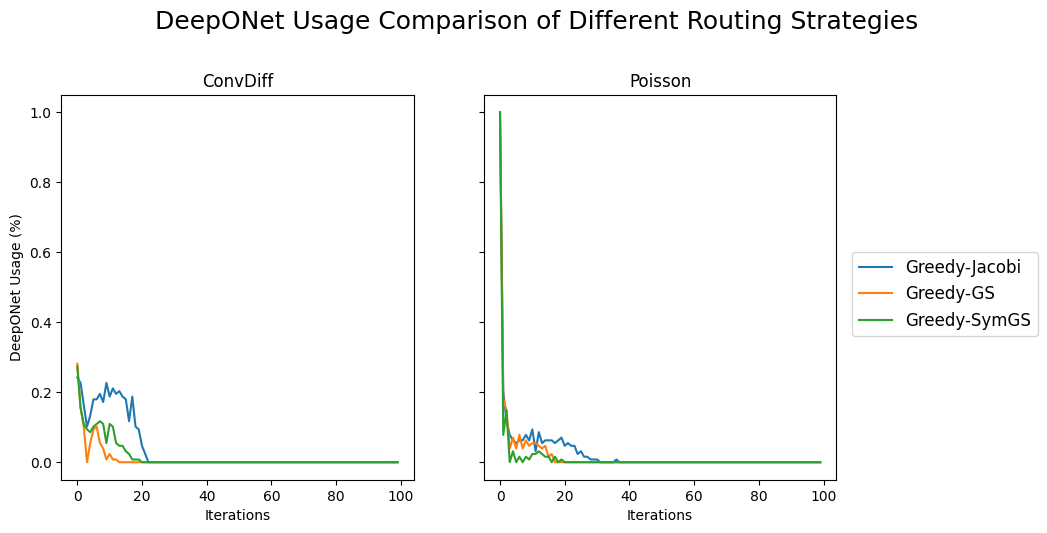
\includegraphics[width=0.5\linewidth]{neurips_images/deeponet_comparison.png}
    \caption{DeepONet usage across iterations for different greedy routing strategies on convection–diffusion (left) and Poisson (right). The variability across iterations highlights the non-uniform, sample-dependent nature of the learned routing strategy. See \Cref{sec:solverdecisions} for detailed routing trajectories. For readability, we display the first 100 iterations (out of 300 total).}
    \label{fig:router_strat}
\end{figure}
% \begin{figure}
%     \resizebox{0.5\textwidth}{!}{\input{}}
% \end{figure}
As shown in \Cref{tab:errorcomparison}, the greedy router achieves the lowest final error and AUC across all solver families, outperforming their single-solver and HINTS counterparts.  Moreover, its performance closely tracks that of the true greedy oracle, indicating that our surrogate-based training procedure effectively approximates the greedy strategy. This can be further seen in the routing visualizations in \Cref{sec:solverdecisions}, which demonstrate that the router learns qualitatively similar strategies to the oracle. The improvements over HINTS are particularly notable: while HINTS can improve over single-solver schedules, it exhibits oscillatory error behavior (See \Cref{fig:errorcomparison}) due to invoking the DeepONet at suboptimal times. In contrast, the greedy routers selectively applies updates that reduce error, resulting in near-monotone convergence. These gains arise from adapting routing decisions across \textit{both} samples for a given PDE and PDEs. For instance, the neural operator is used more frequently in the convection–diffusion setting than in Poisson (\Cref{fig:router_strat}), a behavior that must be manually specified in HINTS but is learned automatically by our method. 
% At the same time, the neural operator is selected only rarely, since classical solvers already achieve strong error reduction in most iterations. 
This shows that improvements stem from selective use of the learned component, rather than frequent invocation as in HINTS.
% That is, some PDEs may be particularly amenable to neural operator interleaving, as seen in the greater operator invocations for the ConvDiff equation than the Poisson equation in \Cref{fig:router_strat}. Leveraging HINTS would require prior knowledge of such behavior, whereas our approach learns it automatically without needing such prescience by the user.
% This improvement is critically linked to the ability of our strategy to dynamically update its routing strategy both across samples and across different PDE settings, unlike HINTS. That is, some PDEs may be particularly amenable to neural operator interleaving, as seen in the greater operator invocations for the ConvDiff equation than in the Poisson equation in \Cref{fig:errorcomparison}; leveraging HINTS even for a single sample would a priori require knowing this fact. Our approach, in contrast, will dynamically learn the appropriate strategy without requiring such prescience by the user.
% We demonstrate that this capacity is clearly leveraged in our experiments, where 
% Notably, the learned routing policy is non-uniform across samples (See \Cref{fig:router_strat}) with the DeepONet correction is often unused after approximately 40 iterations for many instances. This highlights the need for sample-dependent routing and the ineffectiveness of fixed schedules.
\paragraph{Solver Ensembles Experiments:} We consider routing over a collection of more than two solvers. Specifically, we study 
% the performance of our router across 
ensembles $\mathcal{W}$ of increasing size, consisting of a trained DeepONet and a diverse set of numerical solvers, including Jacobi, GS, SymGS, Damped Jacobi $(\omega = 0.67)$ and Successive Over-relaxation (SOR) with $\omega = 1.5$ . Our goal is to evaluate whether enlarging the solver set yields gains beyond pairwise configurations. To this end, we compare $\mathrm{Router}(\mathrm{NO}\cup\mathcal{W})$ against the best pairwise version of our method, $\mathrm{Router}(\mathrm{NO}\cup\{\text{solver}\})$ for solver $\in \mathcal{W}$. As shown in \Cref{tab:errorcomparison2}, larger ensembles often yield improvements over both final error and AUC relative to the best pairwise configuration, indicating that additional solver diversity can be leveraged. The router achieves these gains by learning to route to each member of the ensemble for a non-trivial proportion of the iterates, as measured in \Cref{sec:solverdecisions}. Finally, despite the increased size of the action space, the learned router continues to produce improvements, demonstrating robustness of both the training procedure and the convex surrogate of \Cref{section:surrogate}; true greedy comparisons are deferred to \Cref{sec:moreerrorcomparison}. These results show that our method can scale to richer solver sets, enabling improved performance without sacrificing learnability.
% \paragraph{Solver Ensembles Experiments:} We now consider the setting where we seek to optimally leverage a collection of more than two solvers. The most natural setting where this arises is in parameterizations over solvers, such as across the selection of $\omega$ in successive over-relaxation (SOR) solvers. We, therefore, study the performance of training our router across ensembles of increasing size, consisting of a trained DeepONet and differently parameterized SOR$(\omega)$ solvers, namely with $\omega \in \{1, 1.1, 1.25, 1.4, 1.5\}$. As above, we here seek to demonstrate that the naive alternative, namely of using any individual solver of the ensemble, performs worse than leveraging a learned router. This can be seen in \Cref{tab:errorcomparison2}, across both the final error and AUC metrics. As in \Cref{fig:router_strat}, we demonstrate that the router achieves this improvement by learning to route to each member of the ensemble for a non-trivial proportion of the iterates, explicitly measured in \Cref{sec:solverdecisions}. Critically, the training procedure was precisely the same as that leveraged in the pairwise-routing experiment, demonstrating the robustness of our method and convex surrogate of \Cref{section:surrogate} across settings. In addition, we see that our results yield monotonically decreasing errors as the ensemble size grows, demonstrating that our method can gracefully handle the exponentially growing space of possible routing strategies with enlarged ensembles.
% We also study how the solver ensemble size affects performance by training router with a DeepONet and progressively larger sets of Successive over-relaxation (SOR) solvers with relaxation parameters $\omega \in \{1, 1.1, 1.25, 1.4, 1.5\}$. 
% As shown in \Cref{tab:errorcomparison2}, larger ensembles achieve lower AUC on both equations and outperform its individual solver constituents.
\edit{\paragraph{Wall-clock time-to-solution:} Iteration counts favor methods whose iterations are expensive, so we complement the results above with an end-to-end wall-clock study on a $\caN\times\caN$ grid ($\caN^2$ unknowns) for all five classical solvers and both PDEs, plus a third, harder PDE---anisotropic diffusion $-\epsilon\,\partial_{x_1}^2 u - \partial_{x_2}^2 u = f$ with $\epsilon = 10^{-2}$ on the same periodic domain and data, the standard case in which point smoothers and multigrid with point smoothing degrade; \Cref{sec:wallclock} details the protocol. Three ingredients make the comparison meaningful and the router deployable: (i) all classical solvers are implemented as $O(N^2)$ stencil or cached sparse-triangular sweeps (matching the dense implementations used elsewhere to machine precision), so the classical baseline is not artificially slowed; (ii) the DeepONet corrector acts on the residual through a $64\times 64$ sensor grid with a Fourier trunk basis and is applied scale-equivariantly, so one call solves the smooth half of the spectrum to $\approx 10^{-6}$ at the cost of about $12$ Jacobi or $3$ Gauss--Seidel sweeps and never injects high-frequency error; and (iii) the router is made \emph{cost-aware} through the cost-equalised macro-actions of \Cref{sec:greedy}, and the LSTM is replaced by a router over $6{+}K$ scalar features (log residual, its recent decay rate, the previous action, and call counts) with a two-layer MLP whose decision costs $\approx 5\,\mu$s, trained with the surrogate of \Cref{section:surrogate} to imitate the cost-aware greedy oracle. \Cref{tab:ca_main} reports the median wall-clock time to reach truncation-level relative error $\varepsilon = h^2$, the accuracy beyond which further algebraic refinement is not meaningful on an $N\times N$ grid. The learned router reaches it \caSpSolverMin--\caSpSolverMax faster than the classical solver alone and \caSpHintsMin--\caSpHintsMax faster than HINTS with the published period $\tau{=}25$, in every one of the $\caNumCells$ solver--equation pairings (\Cref{tab:ca_main}); it is also never slower than HINTS with the best period $\tau\in\{5,10,25,50\}$ chosen \emph{a posteriori} on the test set for that pairing (\caSpBestMin--\caSpBestMax; \Cref{tab:ca_vshints}), whereas the best $\tau$ itself varies across pairings and tolerances. The router tracks the cost-aware oracle within \caSpOracleRatioMax in median time, and the iteration-based metrics of \Cref{tab:errorcomparison} carry over to the finer grid (\Cref{tab:ca_auc}). \Cref{fig:ca_usage_main} shows where the gain comes from: the router calls the corrector once at the very start (where the error is smooth and the corrector removes four orders of magnitude at once), spends a solver-dependent number of sweeps on the high-frequency band, and calls it again only if the smooth error re-emerges---between one and three calls in total---while HINTS spends $\tau{-}1$ sweeps before its first call and keeps calling the corrector when it no longer helps. At tolerances far below $h^2$ the undamped-Jacobi pairing is limited by the near-Nyquist modes that neither component damps (\Cref{tab:ca_tol_poisson}), but the router degrades gracefully there because it stops selecting the corrector, whereas fixed schedules keep paying for it (\Cref{sec:wallclock}). Against the classical methods a practitioner would use on these problems (\Cref{tab:ca_baselines}), the router with its best stationary pairing is \caVsMgMin--\caVsMgMax\ faster than geometric multigrid alone, \caVsKrylovMin--\caVsKrylovMax\ faster than the best multigrid-preconditioned Krylov method, and only the FFT direct solve---a method specific to constant-coefficient periodic problems, which we use to compute ground truth---is faster, by \caFftRatioMin--\caFftRatioMax; routing over $\{\mathrm{NO}, \text{multigrid}\}$ is itself \caVsMgEnsMin--\caVsMgEnsMax\ faster than multigrid alone. The gains persist on $256^2$ and $512^2$ grids (\Cref{tab:ca_scaling}) and all comparisons are significant at $p<0.01$ (paired Wilcoxon over instances) and stable across five independent router-training seeds (\Cref{sec:wallclock_stats}). The same construction extends to solver ensembles (\Cref{tab:ca_ens}): over the four ensembles of \Cref{tab:errorcomparison2} and both PDEs, the router over $\mathrm{NO}\cup\mathcal{W}$ matches the best pairwise router of its members to within $\pm15\%$ (ratio of medians \caEnsVsPairMin--\caEnsVsPairMax) without knowing in advance which member is fastest, and is \caEnsVsSolverMin--\caEnsVsSolverMax\ faster than the best member solver alone; the remaining gap to the ensemble oracle, which is faster than every pairwise router, is imitation error in choosing among near-equivalent smoothers (\Cref{sec:wallclock}).}

\begin{table}[t]
\color{red}
\centering
\caption{\edit{Median wall-clock time to truncation-level relative error $\varepsilon = h^2$ on the $\caN\times\caN$ grid, $64$ test instances per cell (paired median speedup over the solver-only baseline in parentheses). ``HINTS (best $\tau$)'' is the best of $\tau\in\{5,10,25,50\}$ chosen per cell on the test set itself. The greedy oracle is the cost-agnostic \Cref{alg:greedy}, the cost-aware oracle is \Cref{alg:greedy} on cost-equalised macro-actions; both use the true error and are not deployable. Bold marks the fastest deployable method in each row; the learned router pays for all of its features and decisions.}}
\resizebox{\textwidth}{!}{\cawcmain}
\label{tab:ca_main}
\end{table}

\begin{figure}[t]
    \centering
    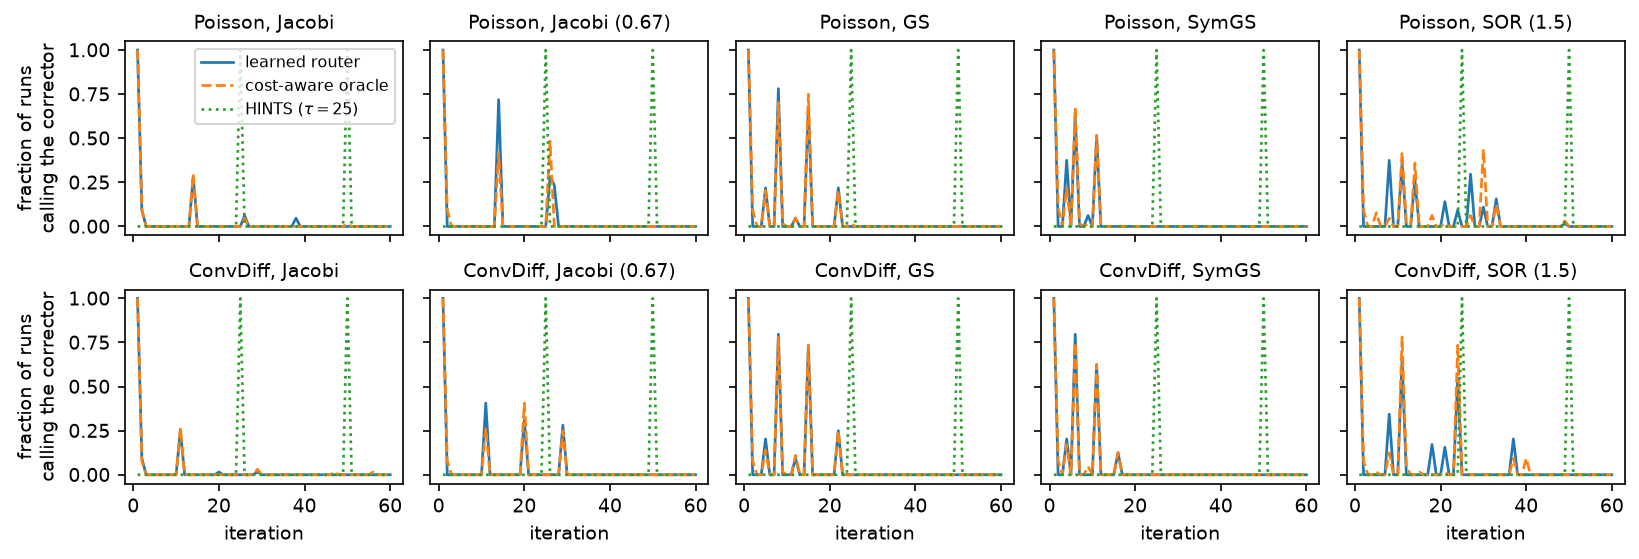
\includegraphics[width=\linewidth]{neurips_images/ca_router_usage.png}
    \caption{\edit{Corrector usage on the $\caN\times\caN$ grid: fraction of test runs that execute a corrector call at each iteration, for the learned router, the cost-aware oracle and HINTS ($\tau{=}25$), for every solver pairing (columns) and both equations (rows).}}
    \label{fig:ca_usage_main}
\end{figure}


Additional experiments are provided in \Cref{sec:moreexperimentalresults}.
% \begin{table}[]
%     \centering
%      \caption{Final error and AUC of squared $L^2$ error for varying numbers of solvers. Values are mean ($\pm$ standard error (s.e.)) over 64 test instances; both mean and s.e. are reported in $\times 10^{-3}$.}
%     \resizebox{\textwidth}{!}{
%     \begin{tabular}{ccccc}
%         \hline
%          Method & \multicolumn{2}{c}{Poisson} & \multicolumn{2}{c}{ConvDiff}\\
%          \hline 
%         \# of Solvers & $\|e^{(T)}_h\| \times 10^3$ & AUC & $\|e^{(T)}_h\| \times 10^3$ & AUC \\
%          \hline
%         SOR (1.0) & 0.003 (0.010) & 0.115 (0.285) & 0.000 (0.000) & 0.035 (0.095) \\
%     SOR (1.25) & 0.000 (0.000) & 0.067 (0.127) & 0.000 (0.000) & 0.017 (0.034) \\
%     SOR (1.5) & 0.000 (0.000) & 0.051 (0.108) & 0.000 (0.000) & 0.015 (0.043) \\
%     SOR (1.75) & 0.000 (0.000) & 0.044 (0.097) & 190.558 (259.625) & 16.153 (15.452) \\
%     SOR (2.0) & 1709.694 (9729.970) & 90.461 (520.960) & 190.558 (259.625) & 16.153 (15.452) \\
%     SOR (1.0), SOR (1.25) & 0.000 (0.001) & 0.075 (0.186) & 0.000 (0.000) & 0.023 (0.070) \\
%     SOR (1.0), SOR (1.25), SOR (1.5) & 0.000 (0.000) & 0.056 (0.111) & 0.000 (0.000) & 0.011 (0.025)   \\
%     SOR (1.0), SOR (1.25), SOR (1.5), SOR (1.75) & 0.000 (0.000) & 0.048 (0.104) & 0.000 (0.000) & 0.013 (0.031) \\
%     SOR (1.0), SOR (1.25), SOR (1.5), SOR (1.75), SOR (2.0) & 0.000 (0.000) & 0.046 (0.101) & inf (nan) & inf (nan)  \\
%          \hline
%     \end{tabular}}
%     \label{tab:errorcomparison2}
% \end{table}
\begin{table}[t]
\centering
\caption{
Final error and AUC of squared $L^2$ error for ensembles of increasing size. $\mathcal{W}$ denotes the set of numerical solvers and
$\mathrm{NO}$ the neural operator (DeepONet). Each $\mathrm{Router}(\mathrm{NO}\cup\mathcal{W})$
is compared against the best pairwise routing using our method, i.e., $\mathrm{Router}(\mathrm{NO}\cup \{\text{solver}\})$ for $\text{solver} \in \mathcal{W}$.
Values are mean ($\pm$ s.e.) over 128 test instances; Error is reported in
$\times 10^{-3}$.
$p$-values from paired one-sided $t$-tests comparing the AUC of the ensemble to that of the best pairwise router.
}
\label{tab:errorcomparison2}

\resizebox{\textwidth}{!}{
\begin{tabular}{llcccccc}
\hline
\multirow{2}{*}{\textbf{$\mathcal{W}$}}
& \multirow{2}{*}{\textbf{Method}}
& \multicolumn{3}{c}{\textbf{Poisson}}
& \multicolumn{3}{c}{\textbf{ConvDiff}} \\
\cline{3-8}
&
& $\|e^{(T)}_h\|\times 10^3$ & AUC & $p$-value (vs pairwise)
& $\|e^{(T)}_h\|\times 10^3$ & AUC & $p$-value (vs pairwise)\\
\hline

\multirow{2}{*}{$\{\text{Jacobi, GS}\}$}
& Best $\mathrm{Router}(\mathrm{NO}\cup \{\text{solver}\})$
& 0.002 (0.004) & 0.083 (0.152) & -
& $<10^{-3}$ & 0.031 (0.078) & -\\
& Router$(\mathrm{NO}\cup\mathcal{W})$
& 0.002 (0.002) & 0.078 (0.132) & $<10^{-3}$ 
& $<10^{-3}$ & 0.021 (0.040) & 0.004 \\
\hline

\multirow{2}{*}{$\{\text{Jacobi, GS, SymGS}\}$}
& Best $\mathrm{Router}(\mathrm{NO}\cup \{\text{solver}\})$
& $<10^{-3}$ & 0.052 (0.102) & -
& $<10^{-3}$ & 0.022 (0.039) & -  \\
& Router$(\mathrm{NO}\cup\mathcal{W})$
& $<10^{-3}$ & 0.041 (0.091) & -$<10^{-3}$
& $<10^{-3}$ & 0.018 (0.035) & $<10^{-3}$ \\
\hline

\multirow{2}{*}{$\{\text{Jacobi, GS, SymGS, Jacobi (0.67)}\}$}
& Best $\mathrm{Router}(\mathrm{NO}\cup \{\text{solver}\})$
& $<10^{-3}$ & 0.052 (0.102) & -
& $<10^{-3}$ & 0.022 (0.039) & -\\
& Router$(\mathrm{NO}\cup\mathcal{W})$
& 0.002 (0.003) & 0.046 (0.083) & 0.004
& $<10^{-3}$ & 0.019 (0.037) & 0.002 \\
\hline

\multirow{2}{*}{$\{\text{Jacobi, GS, SymGS, Jacobi (0.67), SOR (1.5)}\}$}
& Best $\mathrm{Router}(\mathrm{NO}\cup \{\text{solver}\})$
& $<10^{-3}$ & 0.052 (0.143) & -
& $<10^{-3}$ & 0.011 (0.030) & - \\
& Router$(\mathrm{NO}\cup\mathcal{W})$
& $<10^{-3}$ & 0.043 (0.082) & 0.03 
& $<10^{-3}$ & 0.008 (0.019) & 0.004\\
\hline

\end{tabular}
}
\end{table}
% \begin{table}[t]
% \centering
% \caption{
% Final error and AUC of squared $L^2$ error for ensembles of increasing size. Here $\mathcal{W}$ denotes the set of numerical solvers and
% $\mathrm{NO}$ the neural operator (DeepONet). Each $\mathrm{Router}(\mathrm{NO}\cup\mathcal{W})$
% is compared against the best pairwise routing using our method, i.e., $\mathrm{Router}(\mathrm{NO}\cup \{\text{solver}\})$ for $\text{solver} \in \mathcal{W}$.
% Values are mean ($\pm$ s.e.) over 64 test instances; Error is reported in
% $\times 10^{-3}$.
% }
% \label{tab:errorcomparison2}

% \resizebox{\textwidth}{!}{
% \begin{tabular}{llcccc}
% \hline
% \multirow{2}{*}{\textbf{$\mathcal{W}$}}
% & \multirow{2}{*}{\textbf{Method}}
% & \multicolumn{2}{c}{\textbf{Poisson}}
% & \multicolumn{2}{c}{\textbf{ConvDiff}} \\
% \cline{3-6}
% &
% & $\|e^{(T)}_h\|\times 10^3$ & AUC
% & $\|e^{(T)}_h\|\times 10^3$ & AUC \\
% \hline

% \multirow{2}{*}{$\{\text{Jacobi, GS}\}$}
% & Best $\mathrm{Router}(\mathrm{NO}\cup \{\text{solver}\})$
% & 0.003 (0.010) &  0.115 (0.285) &   $< 10^{-3}$ &  0.035 (0.095)\\
% & Router$(\mathrm{NO}\cup\mathcal{W})$
% & 0.001 (0.001) & 0.080 (0.153) & $<10^{-3}$ & 0.031 (0.076) \\
% \hline

% \multirow{2}{*}{$\{\text{Jacobi, GS, SymGS}\}$}
% & Best $\mathrm{Router}(\mathrm{NO}\cup \{\text{solver}\})$
% & $< 10^{-3}$ & 0.074 (0.194)  & $< 10^{-3}$ & 0.026 (0.050)  \\
% & Router$(\mathrm{NO}\cup\mathcal{W})$
% & $<10^{-3}$  & 0.058 (0.101) & $<10^{-3}$  & 0.023 (0.044) \\
% \hline

% \multirow{2}{*}{$\{\text{Jacobi, GS, SymGS, Jacobi (0.67)}\}$}
% & Best $\mathrm{Router}(\mathrm{NO}\cup \{\text{solver}\})$
% & $< 10^{-3}$ & 0.074 (0.194)  & $< 10^{-3}$ & 0.026 (0.050) \\
% & Router$(\mathrm{NO}\cup\mathcal{W})$
% & 0.005 (0.016) & 0.085 (0.218) & $<10^{-3}$  & 0.023 (0.046)\\
% \hline

% \multirow{2}{*}{$\{\text{Jacobi, GS, SymGS, Jacobi (0.67), SOR (1.5)}\}$}
% & Best $\mathrm{Router}(\mathrm{NO}\cup \{\text{solver}\})$
% & $<10^{-3}$ & 0.051 (0.108)
% & $<10^{-3}$ & 0.015 (0.043) \\
% & Router$(\mathrm{NO}\cup\mathcal{W})$
% & $<10^{-3}$  & 0.049 (0.102) & $<10^{-3}$  & 0.010 (0.024)\\
% \hline

% \end{tabular}
% }
% \end{table}
% \begin{table}[t]
% \centering
% \caption{
% Final error and AUC of squared $L^2$ error for ensembles of increasing size. Here $\mathcal{W}$ denotes the SOR relaxation weights and
% $\mathrm{NO}$ the neural operator (DeepONet). Each $\mathrm{Router}(\mathrm{NO}\cup\mathcal{W})$
% is compared only to the best paired routing baseline of the form $\mathrm{Router}(\mathrm{NO}\cup\{\omega\}): \omega \in \mathcal{W}$.
% Values are mean ($\pm$ s.e.) over 64 test instances; Error is reported in
% $\times 10^{-3}$.
% }
% \label{tab:errorcomparison2}

% \resizebox{\textwidth}{!}{
% \begin{tabular}{llcccc}
% \hline
% \textbf{SOR weights $\mathcal{W}$}
% & \textbf{Method}
% & \multicolumn{2}{c}{\textbf{Poisson}}
% & \multicolumn{2}{c}{\textbf{ConvDiff}} \\
% \cline{3-6}
% &
% & $\|e^{(T)}_h\|\times 10^3$ & AUC
% & $\|e^{(T)}_h\|\times 10^3$ & AUC \\
% \hline

% \multirow{2}{*}{$\{1.0,1.1\}$}
% & Best $\mathrm{Router}(\mathrm{NO}\cup\{\omega\})$
% & 0.001 (0.003) & 0.104 (0.248)
% & $<10^{-3}$ & 0.023 (0.043) \\
% & Router$(\mathrm{NO}\cup\mathcal{W})$
% & 0.001 (0.003) & 0.104 (0.226)
% & $<10^{-3}$ & 0.033 (0.112) \\
% \hline

% \multirow{2}{*}{$\{1.0,1.1,1.25\}$}
% & Best $\mathrm{Router}(\mathrm{NO}\cup\{\omega\})$
% & $<10^{-3}$ & 0.067 (0.127)
% & $<10^{-3}$ & 0.017 (0.034) \\
% & Router$(\mathrm{NO}\cup\mathcal{W})$
% & $<10^{-3}$ & 0.073 (0.147)
% & $<10^{-3}$ & 0.026 (0.077) \\
% \hline

% \multirow{2}{*}{$\{1.0,1.1,1.25,1.4\}$}
% & Best $\mathrm{Router}(\mathrm{NO}\cup\{\omega\})$
% & $<10^{-3}$ & 0.063 (0.137)
% & $<10^{-3}$ & 0.017 (0.034) \\
% & Router$(\mathrm{NO}\cup\mathcal{W})$
% & $<10^{-3}$ & 0.056 (0.123)
% & $<10^{-3}$ & 0.012 (0.027) \\
% \hline

% \multirow{2}{*}{$\{1.0,1.1,1.25,1.4,1.5\}$}
% & Best $\mathrm{Router}(\mathrm{NO}\cup\{\omega\})$
% & $<10^{-3}$ & 0.051 (0.108)
% & $<10^{-3}$ & 0.015 (0.043) \\
% & Router$(\mathrm{NO}\cup\mathcal{W})$
% & $<10^{-3}$ & 0.058 (0.135)
% & $<10^{-3}$ & 0.010 (0.024) \\
% \hline

% \end{tabular}
% }
% \end{table}

% \begin{table}[]
%     \centering
%      \caption{Final error and AUC of squared $L^2$ error for varying numbers of solvers. Values are mean ($\pm$ standard error (s.e.)) over 64 test instances; both mean and s.e. are reported in $\times 10^{-3}$.}
%     \resizebox{\textwidth}{!}{
%     \begin{tabular}{ccccc}
%         \hline
%          Method & \multicolumn{2}{c}{Poisson} & \multicolumn{2}{c}{ConvDiff}\\
%          \hline 
%         \# of Solvers & $\|e^{(T)}_h\| \times 10^3$ & AUC & $\|e^{(T)}_h\| \times 10^3$ & AUC \\
%          \hline
%         SOR (1.0) & 0.003 (0.010) & 0.115 (0.285) & $<10^{-3}$ & 0.035 (0.095) \\
%     SOR (1.1) & 0.001 (0.003) & 0.104 (0.248) & $<10^{-3}$ & 0.023 (0.043) \\
%     SOR (1.0), SOR (1.1) &  0.001 (0.003) & 0.104 (0.226) & $<10^{-3}$ & 0.033 (0.112) \\
%     SOR (1.25) & $<10^{-3}$ & 0.067 (0.127) & $<10^{-3}$ & 0.017 (0.034) \\
%     SOR (1.0), SOR (1.1), SOR (1.25) & $<10^{-3}$ & 0.073 (0.147) & $<10^{-3}$ & 0.026 (0.077)  \\
%     SOR (1.4) & $<10^{-3}$ & 0.063 (0.137) & $<10^{-3}$ & 0.018 (0.048) \\
%     SOR (1.0), SOR (1.1), SOR (1.25), SOR (1.4) & $<10^{-3}$ & 0.056 (0.123) & $<10^{-3}$ & 0.012 (0.027) \\
%     SOR (1.5) & $<10^{-3}$ & 0.051 (0.108) & $<10^{-3}$ & 0.015 (0.043) \\
%     SOR (1.0), SOR (1.1), SOR (1.25), SOR (1.4), SOR (1.5) & $<10^{-3}$ & 0.058 (0.135) & $<10^{-3}$ & 0.010 (0.024) \\
%          \hline
%     \end{tabular}}
%     \label{tab:errorcomparison2}
% \end{table}

% \ambuj{experiments section needs a bit more work to be become more defensible. (i) 31 x 31 grid is fine but might be perceived as too small and reviewers might ask what what happens on more realist 64 x 64 or 128 x 128 grids. Can we include some experiments on larger grids in the appendix? }
% \ambuj{(ii) the core theoretical innovation is never tested: why not run oracle greedy, because you can compute the error in hindsight, and compare with the surrogate? that way, the link between core innovation and experiments becomes stronger. }
% \ambuj{(iii) the usage of deeponet is still somewhat low. it will be better if you can investigate it more deeply and shed some insight into why the router ends up using it at the low observed rates in Fig 2}

\section{Discussion} \label{sec:discussion}

We have introduced an adaptive method for selecting solvers that efficiently minimizes the final error of a PDE in iterative methods, opening many directions for future work. Our current DeepONet is trained without accounting for its downstream role in correction term prediction; jointly training the ML solver and router could yield larger gains. Another avenue is to use reinforcement learning to learn a cost-aware routing strategy that optimizes error under compute budgets\edit{; \Cref{sec:greedy,sec:wallclock} show that a myopic cost-aware variant of the greedy rule---\Cref{alg:greedy} on cost-equalised macro-actions---already delivers uniform wall-clock gains, and RL could extend it to non-myopic budgeted routing}. RL would additionally enable extending the ensemble routing to \textit{continuous} parameterization of solvers. Finally, framing routing as an online learning problem could enable adaptation to unknown deployment conditions. 
% where offline training may degrade and fixed schedules like HINTS can perform better. 

\bibliography{mybib}
\bibliographystyle{unsrtnat}




%%%%%%%%%%%%%%%%%%%%%%%%%%%%%%%%%%%%%%%%%%%%%%%%%%%%%%%%%%%%

\appendix
% \section{Background} \label{sec:appbackground}

% \subsection{Multigrid} \label{sec:multigrid}

% Let $A_h, A_{2h}$ represent the coefficient matrix on a fine grid with discretization parameter $h$ and $2h$, $u_h$ and $f_h$ represent the PDE solution and constant vector on a grid discretized by $h$, $R^{2h}_h$ denote the restriction matrix which transfers vectors from a fine grid to a coarse one, and $I^{h}_{2h}$ is the interpolation matrix transfers vectors from a coarse grid to a fine one. In a 2-grid method, a few iterations of the smoother (e.x. Jacobi or Gauss-Seidel) are first applied on the fine grid to approximate the solution of $A_hu_h = f_h$. The residual is then computed as $r_h = f_h - A_hu_h$ and restricted to the coarse grid via $r_{2h} = R^{2h}_hr_h$. The error equation, $A_{2h}e_{2h} = r_{2h}$, is solved on the coarse grid. The resulting estimate of the error is interpolated in the fine grid by $e_h = I^{h}_{2h}e_{2h}$, and the fine grid solution is updated by adding this correction, $u_h = u_h + e_h$. Finally, additional smoothing steps are performed on the fine grid to further reduce any high frequency errors. The preconditioning matrix for two-grid solver is $C_\mathrm{2G} = I^{h}_{2h}A_{2h}^{-1}R^{2h}_h$. More complex strategies for multigrid like V-cycle and W-cycle compute error corrections recursively across multiple grids of varying coarseness %(See \Cref{sec:multigrid} for pseudocode of these methods).

\section{Proofs for \Cref{sec:greedy}} \label{sec:proofgreedy}

\subsection{Proof of Proposition \ref{th:alpha=1}} \label{sec:proofalpha=1}

\begin{proposition} \label{th:alpha=1}
    Any prefix monotonically non-increasing sequence supermodular function $g$ is weakly supermodular with respect to all sequences $S \in \Omega^*$ with $\alpha(S) = 1$
\end{proposition}

\begin{proof}

This proof is adapted from \citet{liberty2017greedy}.

If $g$ is sequence supermodular then,
\begin{align*}
    &g(S) - g(S \ \oplus S' ) \\
    &= \sum_{i = 1}^{|S'|} g(S \ \oplus \left(S'_1, \dots, S'_{i - 1}\right)) - g(S \ \oplus \left(S'_1, \dots, S'_{i}\right)) \\
    &\overset{(a)}{\leq} \sum_{i = 1}^{|S'|} g(S) - g(S \ \oplus  S'_{i}) \\
    &\leq |S'|\max_{i \in [|S'|]} g(S) - g(S \ \oplus  S'_{i})
\end{align*}

(a) by supermodularity


\end{proof}

\subsection{Proof of \Cref{th:suboptgreedy}} \label{sec:proofsuboptgreedy}



\begin{customtheorem}{\ref{th:suboptgreedy}}
    Let $g: \Omega^* \to \mathbb{R}$ be a weakly supermodular function with respect to the optimal solution $O = \argmin_{S \in \Omega^T} h(S)$ with a supermodularity ratio of $\alpha(O)$ and 
    % weak-$\mu$-
    postfix monotonicity. Let the greedy solution of length $T$ be $S^T$. If $\phi_T(\alpha) =  \left(1 - \frac{1}{\alpha T}\right)^T$, then
    \begin{equation*}
        g(S^T) \leq  \left(1 - \phi_T(\alpha(O))\right)
        g(O) +  \phi_T(\alpha(O))g(\emptyset)
    \end{equation*}
    % Equivalently, 
    % \begin{equation*}
    %     \frac{g(\emptyset) - g(S^T)}{g(\emptyset) - g(O)} \geq \mu\left(1 - \left(1 - \frac{1}{\alpha T}\right)^T\right) \geq \mu\left(1 - \frac{1}{e^{\alpha}}\right)
    % \end{equation*}
\end{customtheorem}

\begin{proof}

This proof strategy is inspired by \citet{streeter2008online} and \citet{liberty2017greedy}

\begin{align*}
    g(S^t) -g(O) &\overset{(a)}{\leq} g(S^t) - g(S^t\ \oplus O) \\
    % &= \left(1 - \frac{1}{\mu}\right)g(S^t) + \frac{1}{\mu}\left(g(S^t) - g(S^t\ \oplus O)\right) \\
    &=\sum_{i = 1}^{|O|} g(S^t \oplus \left(o_1, \dots o_{i - 1}\right)) -g(S^t\ \oplus \left(o_1, \dots, o_{i}\right))\\
    &\overset{(b)}{\leq}  \alpha(O)\sum_{i = 1}^{|O|} g(S^t) -g(S^t\ \oplus  o_{i}) \\
    &\leq \alpha(O)|O|\max_{i \in [|O|]} g(S^t) -g(S^t\ \oplus  o_{i}) \\
    &\leq \alpha(O) T g(S^t) -  \alpha(O) T\min_{\omega \in \Omega} g(S^t\ \oplus  \omega) \\
    &= \alpha(O) Tg(S^t) -  \alpha(O) Tg(S^{t + 1})
    % &= Tg(S^t) -  Tg(S^{t + 1}) \\
    % &= T \left(g(S^t) - g(O)\right) - T\left(g(S^{t + 1}) -g(O)\right) \\
    % g(S^{t + 1}) -g(O) &\leq \left(1 - \frac{1}{T}\right)\left(g(S^t) - g(O)\right)
\end{align*}
(a) by $\mu$- postfix monotonicity, (b) by supermodularity. 

After rearranging the inequality, we get:

\begin{align*}
    g(S^{t + 1}) &\leq \frac{1}{\alpha(O) T}\left(g(O) -  \left(\alpha(O) T - 1\right)g(S^t)\right) \\
    &= \frac{1}{\alpha(O) T}g(O) + \left(1 - \frac{1}{\alpha(O) T}\right)g(S^t)
\end{align*}

When recursively applying this inequality, we get:

\begin{align*}
     g(S^{T}) &\leq \frac{1}{\alpha(O) T}g(O)\sum_{i = 0}^{T - 1}\left(1 - \frac{1}{\alpha(O) T}\right)^i + \left(1 - \frac{1}{\alpha(O) T}\right)^Tg(\emptyset) \\
     &= \left(1 - \left(1 - \frac{1}{\alpha(O) T}\right)^T\right)g(O) + \left(1 - \frac{1}{\alpha(O) T}\right)^Tg(\emptyset)
\end{align*}

% \begin{align*}
%     g(S^t) -g(O) &\overset{(a)}{\leq} g(S^t) - \frac{1}{\mu}g(S^t\ \oplus O) \\
%     &= \left(1 - \frac{1}{\mu}\right)g(S^t) + \frac{1}{\mu}\left(g(S^t) - g(S^t\ \oplus O)\right) \\
%     &=\left(1 - \frac{1}{\mu}\right)g(S^t) + \frac{1}{\mu}\sum_{i = 1}^{|O|} g(S^t \oplus \left(o_1, \dots o_{i - 1}\right)) -g(S^t\ \oplus \left(o_1, \dots, o_{i}\right))\\
%     &\overset{(b)}{\leq} \left(1 - \frac{1}{\mu}\right)g(S^t) + \frac{\alpha(O)}{\mu}\sum_{i = 1}^{|O|} g(S^t) -g(S^t\ \oplus  o_{i}) \\
%     &\leq \left(1 - \frac{1}{\mu}\right)g(S^t) + \frac{\alpha(O)|O|}{\mu}\max_{i \in [|O|]} g(S^t) -g(S^t\ \oplus  o_{i}) \\
%     &\leq  \left(1 - \frac{1 - \alpha(O) T}{\mu}\right)g(S^t) -  \frac{\alpha(O) T}{\mu}\min_{\omega \in \Omega} g(S^t\ \oplus  \omega) \\
%     &=  \left(1 - \frac{1 - \alpha(O) T}{\mu}\right)g(S^t) -  \frac{\alpha(O) T}{\mu}g(S^{t + 1})
%     % &= Tg(S^t) -  Tg(S^{t + 1}) \\
%     % &= T \left(g(S^t) - g(O)\right) - T\left(g(S^{t + 1}) -g(O)\right) \\
%     % g(S^{t + 1}) -g(O) &\leq \left(1 - \frac{1}{T}\right)\left(g(S^t) - g(O)\right)
% \end{align*}
% (a) by $\mu$- postfix monotonicity, (b) by supermodularity. 

% After rearranging the inequality, we get:

% \begin{align*}
%     g(S^{t + 1}) &\leq \frac{\mu}{\alpha(O) T}\left(g(O) -  \frac{1 - \alpha(O) T}{\mu}g(S^t)\right) \\
%     &= \frac{\mu}{\alpha(O) T}g(O) + \left(1 - \frac{1}{\alpha(O) T}\right)g(S^t)
% \end{align*}

% When recursively applying this inequality, we get:

% \begin{align*}
%      g(S^{T}) &\leq \frac{\mu}{\alpha(O) T}g(O)\sum_{i = 0}^{T - 1}\left(1 - \frac{1}{\alpha(O) T}\right)^i + \left(1 - \frac{1}{\alpha(O) T}\right)^Tg(\emptyset) \\
%      &= \mu \left(1 - \left(1 - \frac{1}{\alpha(O) T}\right)^T\right)g(O) + \left(1 - \frac{1}{\alpha(O) T}\right)^Tg(\emptyset)
% \end{align*}
\end{proof}

\subsection{Proof of Proposition \ref{th:weaklyalphasupermodular}} \label{sec:proofweaklyalphasupermodular}


% \begin{customproposition}{\ref{th:weaklyalphasupermodular}}
%     If $\|I_N - C_j\mathcal{L}_h^a\| \leq 1$ for all $j \in [K]$, $h$ is (i) prefix monotonically non-increasing and (ii) f is weakly-$\alpha$-supermodular with $$\alpha = \max_{S \in [K]^*: |S| = T}\frac{\left\|I_N - \prod_{t = T}^{1}\left(I_N - C_{S_t}\mathcal{L}_h^a\right)\right\|}{T\left(1 - \max_{t \in [T]}\|I_N - C_{S_t}\mathcal{L}_h^a\|\right) }$$Furthermore, if $I_N - C_j\mathcal{L}_h^a$ is invertible for all $j \in [K]$, $h$ is also postfix monotonically non-increasing.
% \end{customproposition}

\begin{customproposition}{\ref{th:weaklyalphasupermodular}}
     Suppose that for all $j \in [K]$, the error propagation function $I - C_j \circ \mathcal{L}_h^a$ is $\rho_j$-Lipschitz continuous with $\rho_j < 1$, and that $(I - C_j \circ \mathcal{L}_h^a) (0_N) = 0_N$. Then, the function $h$ is weakly supermodular with respect to the optimal solution $O$, with 
     \begin{equation*}
         \alpha(O) = \max\left\{\frac{4}{T - \sum_{i = 1}^{T} \rho_{O_i}^2} , 1\right\}  
     \end{equation*}
     Furthermore, if $I - C_j \circ \mathcal{L}_h^a$ is invertible for all $j \in [K]$, $h$ is also postfix monotonically non-increasing.
\end{customproposition}

\begin{proof}
For brevity, we use the notation $\left(g_1 \circ \dots \circ g_T\right)(x) = \circ_{t = 1}^{T} g_t(x)$, where composition is applied from right to left so that $g_T$ acts first. In this proof, we use a few properties of Lipschitz continuous functions:
\begin{itemize}
    \item \textbf{Property 1:} If $g$ is $\rho$-Lipschitz continuous and $g(0) = 0$, then $\|g(x)\|_2 = \|g(x) - 0\|_2 = \|g(x) - g(0)\|_2 \leq \rho \|x - 0\|_2 = \rho\|x\|_2$
    \item \textbf{Property 2:} If $g_1$ and $g_2$ are Lipschitz continuous functions with Lipschitz constants of $\rho_1$ and $\rho_2$ respectively, the Lipschitz constant of $g_1 + g_2$ and $g_1 - g_2$ is $\rho_1 + \rho_2$.
    \item \textbf{Property 3:} If $g_1$ and $g_2$ are Lipschitz continuous functions with Lipschitz constants of $\rho_1$ and $\rho_2$ respectively, the Lipschitz constant of $g_1 \circ g_2$ is $\rho_1\rho_2$.
\end{itemize}

In order to prove weakly-$\alpha$-supermodularity, we must first prove prefix monotonicity.

\textbf{Prefix monotonicity: } Let $S \preceq S'$ where $S' = S \ \oplus N$.
\begin{align*}
    h(S') &= \left \|\circ_{t = |S'|}^1\left(I - C_{S'_t} \circ \mathcal{L}_h^a\right) \left(e^{(0)}_h\right)\right\|^2_2 \\
    &= \left \|\circ_{t = |S'|}^{|S| + 1}\left(I - C_{S'_t}  \circ \mathcal{L}_h^a\right)\circ \circ_{t = |S|}^1\left(I - C_{S'_t}  \circ \mathcal{L}_h^a\right) \left(e^{(0)}_h\right)\right\|^2_2 \\
    &\overset{(a)}{\leq}\left( \prod_{t = |S| + 1 }^{|S'|} \rho_{S'_t}^2 \right)\left\|\circ_{t = |S|}^1\left(I - C_{S_t} \circ \mathcal{L}_h^a\right) \left(e^{(0)}_h\right)\right\|^2_2 \\
    &\leq h(S)
\end{align*}
(a) by Property 1


\textbf{Weak supermodularity: } 
% \paragraph{ } 
We will upper bound $\alpha(O)$ by providing an upper bound for $ h(S) - h(S\ \oplus O) $ and a lower bound for $\sum_{i = 1}^T h(S) - h(S\ \oplus O_i) $. 
\begin{align*}
    h(S) - h(S\ \oplus O) &=  \left \|\circ_{t = |S|}^1\left(I - C_{S_t} \circ \mathcal{L}_h^a\right) \left(e^{(0)}_h\right)\right\|^2_2 -  \left \|\circ_{t = |O|}^{1}\left(I- C_{O_t} \circ\mathcal{L}_h^a\right) \circ \circ_{t = |S|}^1\left(I - C_{S_t} \circ \mathcal{L}_h^a\right)\left(e^{(0)}_h\right)\right\|^2_2 \\
    &\overset{(a)}{\leq} \left \|\circ_{t = |S|}^1\left(I - C_{S_t} \circ \mathcal{L}_h^a\right) \left(e^{(0)}_h\right)-\circ_{t = |O|}^{1}\left(I - C_{O_t} \circ \mathcal{L}_h^a\right) \circ \circ_{t = |S|}^1\left(I - C_{S_t} \circ \mathcal{L}_h^a\right)\left(e^{(0)}_h\right)\right\|^2_2 \\
    &=  \left \| \left(I -\circ_{t = |O|}^{1}\left(I - C_{O_t}\circ\mathcal{L}_h^a\right) \right)\circ  \circ_{t = |S|}^1\left(I - C_{S_t}\circ\mathcal{L}_h^a\right) \left(e^{(0)}_h\right)\right\|^2_2 \\
    &\overset{(b)}{\leq}  \left(1 + \prod_{t = 1}^{|O|}\rho_{O_t}\right)^2\left\| \circ_{t = |S|}^1\left(I - C_{S_t} \circ \mathcal{L}_h^a\right) \left(e^{(0)}_h\right)\right\|^2_2 \\
    &\overset{(c)}{\leq } 4 \left\| \circ_{t = |S|}^1\left(I - C_{S_t} \circ \mathcal{L}_h^a\right) \left(e^{(0)}_h\right)\right\|^2_2
\end{align*}
% \begin{align*}
%     h(S) - h(S\ \oplus S') &=  \left \|\circ_{t = |S|}^1\left(I - C_{S_t} \circ \mathcal{L}_h^a\right) \left(e^{(0)}_h\right)\right\|^2_2 -  \left \|\circ_{t = |S'|}^{1}\left(I- C_{S'_t} \circ\mathcal{L}_h^a\right) \circ \circ_{t = |S|}^1\left(I - C_{S_t} \circ \mathcal{L}_h^a\right)\left(e^{(0)}_h\right)\right\|^2_2 \\
%     &\overset{(a)}{\leq} \left \|\circ_{t = |S|}^1\left(I - C_{S_t} \circ \mathcal{L}_h^a\right) \left(e^{(0)}_h\right)-\circ_{t = |S'|}^{1}\left(I - C_{S'_t} \circ \mathcal{L}_h^a\right) \circ \circ_{t = |S|}^1\left(I - C_{S_t} \circ \mathcal{L}_h^a\right)\left(e^{(0)}_h\right)\right\|^2_2 \\
%     &=  \left \| \left(I -\circ_{t = |S'|}^{1}\left(I - C_{S'_t}\circ\mathcal{L}_h^a\right) \right)\circ  \circ_{t = |S|}^1\left(I - C_{S_t}\circ\mathcal{L}_h^a\right) \left(e^{(0)}_h\right)\right\|^2_2 \\
%     &\overset{(b)}{\leq}  \left(1 + \prod_{t = 1}^{|S'|}\rho_{S'_t}\right)^2\left\| \circ_{t = |S|}^1\left(I - C_{S_t} \circ \mathcal{L}_h^a\right) \left(e^{(0)}_h\right)\right\|^2_2 \\
%     &\overset{(c)}{\leq } 4 \left\| \circ_{t = |S|}^1\left(I - C_{S_t} \circ \mathcal{L}_h^a\right) \left(e^{(0)}_h\right)\right\|^2_2
% \end{align*}

(a) by reverse triangle property and $h(S) - h(S\ \oplus S') > 0$ by prefix monotonicity, (b) since the Lipschitz constant of $I -\circ_{t = |S'|}^{1}\left(I - C_{S'_t}\circ\mathcal{L}_h^a\right)$ is $1 + \prod_{t = 1}^{|S'|}\rho_{S'_t}$ by Property 2 and 3, (c) since $\rho_j < 1$


To lower bound $\sum_{i = 1}^{|O|} h(S) - h(S\ \oplus O_i) $
\begin{align*}
    \sum_{i = 1}^{|O|} h(S) - h(S\ \oplus O_i) &= \sum_{i = 1}^{|O|} \left \|\circ_{t = |S|}^1\left(I - C_{S_t} \circ \mathcal{L}_h^a\right) \left(e^{(0)}_h\right)\right\|^2_2 - \left \|\left(I - C_{O_i} \circ \mathcal{L}_h^a\right) \circ \circ_{t = |S|}^1\left(I - C_{S_t} \circ\mathcal{L}_h^a\right) \left(e^{(0)}_h\right)\right\|^2_2  \\
    &\geq \sum_{i = 1}^{|O|} \left \|\circ_{t = |S|}^1\left(I - C_{S_t} \circ\mathcal{L}_h^a\right) \left(e^{(0)}_h\right)\right\|^2_2 - \rho_{O_i}^2\left\|\circ_{t = |S|}^1\left(I - C_{S_t}\circ\mathcal{L}_h^a\right) \left(e^{(0)}_h\right)\right\|^2_2 \\
    &= \left \|\circ_{t = |S|}^1\left(I_N - C_{S_t}\circ\mathcal{L}_h^a\right) \left(e^{(0)}_h\right)\right\|^2_2 \left(T - \sum_{i = 1}^{T} \rho_{O_i}^2\right) 
\end{align*}
% \begin{align*}
%     \max_i h(S) - h(S\ \oplus S'_i) &= \left \|\circ_{t = |S|}^1\left(I - C_{S_t} \circ \mathcal{L}_h^a\right) \left(e^{(0)}_h\right)\right\|^2_2 - \min_i \left \|\left(I - C_{S_i'} \circ \mathcal{L}_h^a\right) \circ \circ_{t = |S|}^1\left(I - C_{S_t} \circ\mathcal{L}_h^a\right) \left(e^{(0)}_h\right)\right\|^2_2  \\
%     &\geq \left \|\circ_{t = |S|}^1\left(I - C_{S_t} \circ\mathcal{L}_h^a\right) \left(e^{(0)}_h\right)\right\|^2_2 - \min_i \rho_{S_i'}^2\left\|\circ_{t = |S|}^1\left(I - C_{S_t}\circ\mathcal{L}_h^a\right) \left(e^{(0)}_h\right)\right\|^2_2 \\
%     &= \left(1 - \min_i \rho_{S_i'}^2\right) \left \|\circ_{t = |S|}^1\left(I_N - C_{S_t}\circ\mathcal{L}_h^a\right) \left(e^{(0)}_h\right)\right\|^2_2 
% \end{align*}

Finally,

\begin{align*}
    \frac{h(S) - h(S\ \oplus O)}{T\max_i h(S) - h(S\ \oplus O_i)} &\leq \max\left\{ \frac{4\left\| \circ_{t = |S|}^1\left(I - C_{S_t} \circ \mathcal{L}_h^a\right) \left(e^{(0)}_h\right)\right\|^2_2}{\left \|\circ_{t = |S|}^1\left(I_N - C_{S_t}\circ\mathcal{L}_h^a\right) \left(e^{(0)}_h\right)\right\|^2_2 \left(T - \sum_{i = 1}^{T} \rho_{O_i}^2\right) }, 1\right\}\\
    &= \max\left\{\frac{4}{T - \sum_{i = 1}^{T} \rho_{O_i}^2} , 1\right\} 
\end{align*}

\textbf{Postfix monotonicity: } Let $S' = S \ \oplus N$. 

% Consider a function $\tilde{h}^{-1}(z)$ for $z \in \mathbb{R}^N$ be a function such that $\tilde{h}^{-1}(h(N)) = $

%Let $b$ a function such that $b \ \circ  \circ_{t = |N|}^{1}\left(I - C_{N_t}\circ\mathcal{L}_h\right) e^{(0)} = e^{(0)}$

\begin{align*}
    h(S') &= \left \|\circ_{t = |S'|}^1\left(I - C_{S'_t}\circ\mathcal{L}_h\right) e^{(0)}_h\right\|^2_2 \\
    &= \left \|\circ_{t = |N|}^{1}\left(I - C_{N_t}\circ \mathcal{L}_h\right)\circ \circ_{t = |S|}^1\left(I - C_{S_t}\circ \mathcal{L}_h\right) e^{(0)}_h\right\|^2_2 \\
    &\overset{(a)}{=}  \left \|\circ_{t = |N|}^{1}\left(I - C_{N_t} \circ \mathcal{L}_h\right)\circ \circ_{t = |S|}^1\left(I - C_{S_t}\circ\mathcal{L}_h\right)\circ\left(\circ_{t = |N|}^{1}\left(I - C_{N_t}\circ\mathcal{L}_h\right)\right)^{-1}\circ \circ_{t = |N|}^{1}\left(I - C_{N_t}\circ\mathcal{L}_h\right) e^{(0)}_h\right\|^2_2 \\
    &\leq \prod_{t = 1}^{|N|} \rho^2_{N_t} \prod_{t = 1}^{|S|} \rho^2_{S_t} \prod_{t = 1}^{|N|} \rho^{-2}_{N_t}  \left\|\circ_{t = |N|}^{1}\left(I - C_{N_t}\circ\mathcal{L}_h\right) e^{(0)}_h\right\|^2_2 \\
    % &\leq \left \|\prod_{t = |N|}^{1}\left(I_N - C_{N_t}\mathcal{L}_h\right)\right\|^2_2\left \|\prod_{t = |S|}^1\left(I_N - C_{S_t}\mathcal{L}_h\right)\right\|^2_2\left \|\prod_{t = |N|}^{1}\left(I_N - C_{N_t}\mathcal{L}_h\right)\right\|^{-2}_2\left \| \prod_{t = |N|}^{1}\left(I_N - C_{N_t}\mathcal{L}_h\right)e^{(0)}\right\|^2_2 \\
    % &\leq \circ_{t = |S|}^{1}\left \|\left(I - C_{S_t}\circ\mathcal{L}_h\right) \right\|^2_2 \left\|\circ_{t = |N|}^1\left(I - C_{N_t}\circ\mathcal{L}_h\right) e^{(0)}\right\|^2_2 \\
    &\leq h(N)
\end{align*}

% \begin{align*}
%     h(S') &= \left \|\circ_{t = |S'|}^1\left(I - C_{S'_t}\circ\mathcal{L}_h\right) e^{(0)}_h\right\|^2_2 \\
%     &= \left \|\circ_{t = |N|}^{1}\left(I - C_{N_t}\circ \mathcal{L}_h\right)\circ \circ_{t = |S|}^1\left(I - C_{S_t}\circ \mathcal{L}_h\right) e^{(0)}_h\right\|^2_2 \\
%     &\overset{(a)}{=}  \left \|\circ_{t = |N|}^{1}\left(I - C_{N_t} \circ \mathcal{L}_h\right)\circ \circ_{t = |S|}^1\left(I - C_{S_t}\circ\mathcal{L}_h\right)\circ\left(\circ_{t = |N|}^{1}\left(I - C_{N_t}\circ\mathcal{L}_h\right)\right)^{-1}\circ \circ_{t = |N|}^{1}\left(I - C_{N_t}\circ\mathcal{L}_h\right) e^{(0)}\right\|^2_2 \\
%     &\leq \prod_{t = 1}^{|N|} \rho^2_{N_t} \prod_{t = 1}^{|S|} \rho^2_{S_t} \rho^2(g)  \left\|\circ_{t = |N|}^{1}\left(I - C_{N_t}\circ\mathcal{L}_h\right) e^{(0)}\right\|^2_2 \\
%     % &\leq \left \|\prod_{t = |N|}^{1}\left(I_N - C_{N_t}\mathcal{L}_h\right)\right\|^2_2\left \|\prod_{t = |S|}^1\left(I_N - C_{S_t}\mathcal{L}_h\right)\right\|^2_2\left \|\prod_{t = |N|}^{1}\left(I_N - C_{N_t}\mathcal{L}_h\right)\right\|^{-2}_2\left \| \prod_{t = |N|}^{1}\left(I_N - C_{N_t}\mathcal{L}_h\right)e^{(0)}\right\|^2_2 \\
%     % &\leq \circ_{t = |S|}^{1}\left \|\left(I - C_{S_t}\circ\mathcal{L}_h\right) \right\|^2_2 \left\|\circ_{t = |N|}^1\left(I - C_{N_t}\circ\mathcal{L}_h\right) e^{(0)}\right\|^2_2 \\
%     &\leq h(N)
% \end{align*}

(a) due the invertibility of $I_N - C_j\mathcal{L}_h$

\end{proof}

\subsection{Proof of \Cref{th:simultaneousallocation}} \label{sec:proofsimultaneousallocation}

\begin{lemma} \label{th:simultaneousallocation}
     Let $\left(I - C_j \mathcal{L}_{h}^a\right) = P\Lambda_jP^{-1}$ where $P$ is an orthogonal matrix and $\Lambda_j = \mathrm{diag}(\lambda_{j1}, \dots, \lambda_{jN})$. If $P^{-1}e^{(0)}_h = z$, then the following equality holds:
     \begin{equation} \label{eq:simultaneous}
          h(S) = \sum_{i = 1}^N z_i^2 \prod_{j = 1}^K \lambda_{ji}^{2m_j(S)}
          % \qquad\mathrm{s.t}\qquad \sum_{k=1}^{K} m_k = T 
     \end{equation}
     where $m_j(S) = \sum_{t= 1}^{|S|}\1_{S_t = j}$
\end{lemma}

\begin{proof}

\begin{align*}
    h(S) &= \left\|\prod_{t = |S|}^1\left(I_N - C_{S_t} \mathcal{L}_{h}^a\right)  e^{(0)}_h \right\|^2 \\
    &=  \left\|\prod_{t = |S|}^1\left(P\Lambda_{S_t}P^{-1}\right)  e^{(0)}_h \right\|^2 \\
    &=  \left\|P\prod_{t = |S|}^1\Lambda_{S_t}P^{-1}  e^{(0)}_h \right\|^2 \\
    &= \left\|\prod_{t = |S|}^1\Lambda_{S_t}P^{-1}  e^{(0)}_h \right\|^2\\
    &=  \sum_{i = 1}^N z_i^2 \prod_{t = T}^1 \lambda_{S_ti}^2 \\
    &=  \sum_{i = 1}^N z_i^2 \prod_{j = 1}^K \lambda_{ji}^{2m_j(S)} 
    % &= \min_{\mathbf{m} \in\mathbb{N}^{K}}\quad \sum_{j = 1}^N z_i^2 \exp \left\{\sum_{k = 1}^K m_k \log \lambda_{kj}^{2}\right\}
    % \qquad\mathrm{s.t}\qquad \sum_{k=1}^{K} m_k = T
\end{align*}

\end{proof}

\subsection{Proof of \Cref{th:simultaneoussupermodular}} \label{sec:proofsimultaneoussupermodular}
\begin{customproposition}{\ref{th:simultaneoussupermodular}}
    Let $\|I_N - C_j\mathcal{L}_h^a\| \leq 1$ for all $j \in [K]$ and $\left(I - C_j \mathcal{L}_{h}^a\right) = P\Lambda_jP^{-1}$. Then, $h$ is supermodular. 
\end{customproposition}

\begin{proof}

Let $S \preceq S'$ where $S' = S \ \oplus B$. By \Cref{th:simultaneousallocation},
\begin{align*}
    h(S) &= \sum_{i = 1}^N z_i^2 \prod_{j = 1}^K \lambda_{ji}^{2m_j(S)} 
\end{align*}
where $m_j(S) = \sum_{t = 1}^{|S|} \1_{S_t = j}$ be the number of times a sequence $S$ calls the solver $j$. Recall that $h$ is considered sequence supermodular if $\forall S', S \in \Omega^*$ such that $S \preceq S'$, it holds that
\begin{align*}
    h(S) - h(S \ \oplus \omega ) \geq h(S') - h(S' \ \oplus \omega )
\end{align*}
% Without loss of generality, let's assume that $\omega$ that will be appended to $S, S'$ is $1$.
\begin{align*}
    h(S) - h(S \ \oplus \omega) &= \sum_{i = 1}^N z_i^2 \prod_{j = 1}^K \lambda_{ji}^{2m_j(S)} - \sum_{i = 1}^N z_i^2 \lambda_{\omega i}^{2}\prod_{k = 1}^K \lambda_{ji}^{2m_j(S)} \\
    &=  \sum_{i = 1}^N \left(1 - \lambda_{\omega i}^2\right) z_i^2 \prod_{j = 1}^K \lambda_{ji}^{2m_j(S)}
\end{align*}
Similarly, 
\begin{align*}
    h(S') - h(S \ \oplus \omega) &= \sum_{i = 1}^N \left(1 - \lambda_{\omega i}^2\right) z_i^2 \prod_{j = 1}^K \lambda_{ji}^{2m_j(S')} \\
    &\overset{(a)}{=}  \sum_{i = 1}^N \left(1 - \lambda_{\omega i}^2\right) z_i^2 \prod_{j = 1}^K \lambda_{ji}^{2\left(m_j(S) + m_j(B)\right)} \\
    &\overset{(b)}{\leq } \sum_{i = 1}^N \left(1 - \lambda_{\omega i}^2\right) z_i^2 \prod_{j = 1}^K \lambda_{ji}^{2m_j(S)} \\
    &= h(S) - h(S \ \oplus \omega)
\end{align*}


(a) Since $m_j(S') = \sum_{t = 1}^{|S'|} \1_{S_t' = j} = \sum_{t = 1}^{|S|} \1_{S_t' = j} + \sum_{t = |S|}^{|S'|} \1_{S_t' = j} = \sum_{t = 1}^{|S|} \1_{S_t = k} + \sum_{t = 1}^{|B|} 1_{B_t = j} = m_j(S) + m_j(B)$, (b) since $\rho(I_N - C_j \mathcal{L}_h^a) < 1$ and $m_j(B) \geq 0$ for all $j \in [K]$

\end{proof}


\section{Proofs for \Cref{sec:approxgreedy}} \label{sec:proofapproxgreedy}

\subsection{Proof of \Cref{th:routingequivalence}} \label{sec:proofroutingequivalence}

\begin{lemma} \label{th:routingequivalence}

For any set of preconditioning functions $\mathcal{C}$, any discrete operator $\mathcal{L}_h^a$, any router $r$, any $a_h, f_h, u_h^{(t)}, u_h \in \mathcal{A} \times \mathcal{F} \times \mathcal{U} \times \mathcal{U}$, the following equality holds true:
\begin{align*}
     l_{\text{route}}\left(r, a_h, f_h, u^{(t)}_h, u_h\right) = &\sum_{j = 1}^K \sum_{k = 1}^K\left\|\left( I - C_{k} \circ \mathcal{L}_{h}^a\right)\left(u_h - u^{(t)}_h\right)\right\|^2_2\1_{k\neq j}\1_{r(a_h, f_h, u^{(t)}_h) \neq j} \\
     &-\left(K - 2\right)\sum_{j = 1}^K\left\|\left( I - C_{j} \circ \mathcal{L}_{h}^a\right)\left(u_h - u^{(t)}_h\right)\right\|^2_2
\end{align*}
    
\end{lemma}

\begin{proof}
Note that $\sum_{j = 1}^K \1_{r(a_h, f_h, u^{(t)}_h) \neq j}= K - 1$
\begin{align*}
    l_{\text{route}}\left(r, a_h, f_h, u^{(t)}_h, u_h\right) &= \sum_{j = 1}^K \left\|\left( I - C_{j} \circ \mathcal{L}_{h}^a\right)\left(u_h - u^{(t)}_h\right)\right\|^2_2\1_{r(a_h, f_h, u^{(t)}_h) = j} \\
    &= \sum_{j = 1}^K \left\|\left( I - C_{j} \circ \mathcal{L}_{h}^a\right)\left(u_h - u^{(t)}_h\right)\right\|^2_2 - \sum_{j = 1}^K \left\|\left( I - C_{j} \circ \mathcal{L}_{h}^a\right)\left(u_h - u^{(t)}_h\right)\right\|^2_2\1_{r(a_h, f_h, u^{(t)}_h) \neq j} \\
    &= \sum_{j = 1}^K \left\|\left( I - C_{j} \circ \mathcal{L}_{h}^a\right)\left(u_h - u^{(t)}_h\right)\right\|^2_2 - \sum_{j = 1}^K \left\|\left( I - C_{j} \circ \mathcal{L}_{h}^a\right)\left(u_h - u^{(t)}_h\right)\right\|^2_2\1_{r(a_h, f_h, u^{(t)}_h) \neq j} \\
    &+ \left(K - 1\right)\sum_{k = 1}^K\left\|\left( I - C_{k} \circ \mathcal{L}_{h}^a\right)\left(u_h - u^{(t)}_h\right)\right\|^2_2 - \left(K - 1\right)\sum_{k = 1}^K\left\|\left( I - C_{k} \circ \mathcal{L}_{h}^a\right)\left(u_h - u^{(t)}_h\right)\right\|^2_2 \\
    &= \sum_{j = 1}^K \left\|\left( I - C_{j} \circ \mathcal{L}_{h}^a\right)\left(u_h - u^{(t)}_h\right)\right\|^2_2 - \sum_{j = 1}^K \left\|\left( I - C_{j} \circ \mathcal{L}_{h}^a\right)\left(u_h - u^{(t)}_h\right)\right\|^2_2\1_{r(a_h, f_h, u^{(t)}_h) \neq j} \\
    &+ \sum_{j = 1}^K\1_{r(a_h, f_h, u^{(t)}_h) \neq j}\sum_{k = 1}^K\left\|\left( I - C_{k} \circ \mathcal{L}_{h}^a\right)\left(u_h - u^{(t)}_h\right)\right\|^2_2 \\
    &- \left(K - 1\right)\sum_{k = 1}^K\left\|\left( I - C_{k} \circ \mathcal{L}_{h}^a\right)\left(u_h - u^{(t)}_h\right)\right\|^2_2 \\
\end{align*}
\begin{align*}
    &= \sum_{j = 1}^K\left(\sum_{k = 1}^K\left\|\left( I - C_{k} \circ \mathcal{L}_{h}^a\right)\left(u_h - u^{(t)}_h\right)\right\|^2_2  - \left\|\left( I - C_{j} \circ \mathcal{L}_{h}^a\right)\left(u_h - u^{(t)}_h\right)\right\|^2_2\right)\1_{r(a_h, f_h, u^{(t)}_h) \neq j} \\
    &- \left(K - 2\right)\sum_{k = 1}^K\left\|\left( I - C_{k} \circ \mathcal{L}_{h}^a\right)\left(u_h - u^{(t)}_h\right)\right\|^2_2 \\
    &=\sum_{j = 1}^K\sum_{k = 1}^K\left\|\left( I - C_{k} \circ \mathcal{L}_{h}^a\right)\left(u_h - u^{(t)}_h\right)\right\|^2_2\1_{k\neq j}\1_{r(a_h, f_h, u^{(t)}_h) \neq j} \\
    &- \left(K - 2\right)\sum_{k = 1}^K\left\|\left( I - C_{k} \circ \mathcal{L}_{h}^a\right)\left(u_h - u^{(t)}_h\right)\right\|^2_2
 \end{align*}
\end{proof}


\subsection{Proof of \Cref{th:upperbound}} \label{sec:proofupperbound}

\begin{proposition} \label{th:upperbound}
    For any router $r$ defined by $r(a, f, u^{(t)}) = \text{argmax}_{j \in [K]} g_j(a, f, u^{(t)})$, any $a_h \in \mathcal{A}$, $f_h \in \mathcal{F}$, and $u_h^{(t)}, u_h \in \mathcal{U}$, the routing loss $l_{\text{route}}$ satisfies:
    \begin{equation*}
        \log(2)l_{\text{route}}\left(r, a_h, f_h, u^{(t)}_h, u_h\right)\leq \Psi(\mathbf{g}, a_h, f_h, u_h^{(t)}, u_h) 
    \end{equation*}
\end{proposition}


\begin{proof}

By \Cref{th:routingequivalence}, we know that

\begin{align*}
    \log(2)l_{\text{route}}\left(r, a_h, f_h, u^{(t)}_h, u_h\right) = &\log(2)\sum_{j = 1}^K \sum_{k = 1}^K\left\|\left( I - C_{k} \circ \mathcal{L}_{h}^a\right)\left(u_h - u^{(t)}_h\right)\right\|^2_2\1_{k\neq j}\1_{r(a_h, f_h, u^{(t)}_h) \neq j} \\
     &-\log(2)\left(K - 2\right)\sum_{j = 1}^K\left\|\left( I - C_{j} \circ \mathcal{L}_{h}^a\right)\left(u_h - u^{(t)}_h\right)\right\|^2_2 \\
     &\leq \log(2)\sum_{j = 1}^K \sum_{k = 1}^K\left\|\left( I - C_{k} \circ \mathcal{L}_{h}^a\right)\left(u_h - u^{(t)}_h\right)\right\|^2_2\1_{k\neq j}\1_{r(a_h, f_h, u^{(t)}_h) \neq j} \\
     &\overset{(a)}{\leq} -\sum_{j = 1}^K \sum_{k = 1}^K\left\|\left( I - C_{k} \circ \mathcal{L}_{h}^a\right)\left(u_h - u^{(t)}_h\right)\right\|^2_2\1_{k\neq j}\log\left(\frac{\exp\left(g_j(a, f, u^{(t)})\right)}{\sum_{k = 1}^K\exp\left(g_k(a, f, u^{(t)})\right)}\right) \\
     &= \Psi(\mathbf{g}, a_h, f_h, u_h^{(t)}, u_h)
\end{align*}
(a) if $r(a_h, f_h, u^{(t)}_h) \neq j$, $\frac{\exp\left(g_j(a, f, u^{(t)})\right)}{\sum_{k = 1}^K\exp\left(g_k(a, f, u^{(t)})\right)} < 0.5$ which implies that $-\log\left(\frac{\exp\left(g_j(a, f, u^{(t)})\right)}{\sum_{k = 1}^K\exp\left(g_k(a, f, u^{(t)})\right)}\right)  \geq \log(2)\1_{r(a_h, f_h, u^{(t)}_h) \neq j}$

\end{proof}


\subsection{Proof of \Cref{th:consistency}} \label{sec:proofconsistency}

\begin{customtheorem}{\ref{th:consistency}}
    Let $\Tilde{c}_j(a_h, u^{(t)}_h, u_h) < \Bar{E} < \infty$  for all $j \in [K]$. If there exists $j\in [K]$ such that $\Tilde{c}_j(a_h, u^{(t)}_h, u_h) > E_{min} > 0$, then, for any collection of solvers $\{C_j\}_{j= 1}^K$ and linear discrete operator $\mathcal{L}_h^a$, $\Psi$ is Bayes consistent surrogate for $l_{\text{route}}$.
\end{customtheorem}

\begin{proof}

For a given $a_h, f_h$, let $u_h$ be $\mathcal{G}_h\left(a_h, f_h\right)$ where $\mathcal{G}_h$ denotes the solution operator acting on the grid $G_h$. Furthermore, let's consider routers of the form
\begin{equation*}
    r(a, f, u^{(t)}) = \text{argmax}_{j \in [K]} g_j(a, f, u^{(t)})
\end{equation*}

For a given $a_h, f_h, u_h^{(t)} \in \mathcal{A} \times \mathcal{F} \times \mathcal{U}$, let the optimal loss under $l_{\text{route}}$ be $l_{\text{route}}^*\left(a_h, f_h, u^{(t)}_h\right) = \inf_{\Tilde{r}} l_{\text{route}}\left(\tilde{r}, a_h, f_h, u^{(t)}_h, \mathcal{G}_h\left(a_h, f_h\right)\right)$. Similarly, let the optimal loss under $\Psi$ be $\Psi^*\left(a_h, f_h, u^{(t)}_h\right) = \inf_{\Tilde{\mathbf{g}}} \Psi\left(\tilde{\mathbf{g}}, a_h, f_h, u^{(t)}_h, \mathcal{G}_h\left(a_h, f_h\right)\right)$. Let $B_j(a_h, f_h, u^{(t)}_h) = \sum_{k = 1}^K\left\|\left( I - C_{k} \circ \mathcal{L}_{h}^a\right)\left(\mathcal{G}_h\left(a_h, f_h\right) - u^{(t)}_h\right)\right\|^2_2\1_{k\neq j}$.

\begin{align*}
    &l_{\text{route}}\left(r, a_h, f_h, u^{(t)}_h, \mathcal{G}_h\left(a_h, f_h\right)\right) - l_{\text{route}}^*\left(a_h, f_h, u^{(t)}_h\right) \\
    &\overset{(a)}{=} \sum_{j = 1}^K\sum_{k = 1}^K\left\|\left( I - C_{k} \circ \mathcal{L}_{h}^a\right)\left(u_h - u^{(t)}_h\right)\right\|^2_2\1_{k\neq j}\1_{r(a_h, f_h, u^{(t)}_h) \neq j}  -\left(K - 2\right)\sum_{j = 1}^K\left\|\left( I - C_{j} \circ \mathcal{L}_{h}^a\right)\left(u_h - u^{(t)}_h\right)\right\|^2_2 \\
    &\quad- \inf_{\Tilde{r}} \sum_{j = 1}^K\sum_{k = 1}^K\left\|\left( I - C_{k} \circ \mathcal{L}_{h}^a\right)\left(u_h - u^{(t)}_h\right)\right\|^2_2\1_{k\neq j}\1_{\tilde{r}(a_h, f_h, u^{(t)}_h) \neq j}  +\left(K - 2\right)\sum_{j = 1}^K\left\|\left( I - C_{j} \circ \mathcal{L}_{h}^a\right)\left(u_h - u^{(t)}_h\right)\right\|^2_2 \\
    &= \sum_{j = 1}^K B_j(a_h, f_h, u^{(t)}_h)\1_{r(a_h, f_h, u^{(t)}_h) \neq j} - \inf_{\Tilde{r}} \sum_{j = 1}^KB_j(a_h, f_h, u^{(t)}_h)\1_{\tilde{r}(a_h, f_h, u^{(t)}_h) \neq j}  \\
    &= \sum_{k = 1}^K B_k(a_h, f_h, u^{(t)}_h)\left(\sum_{j = 1}^K \frac{B_j(a_h, f_h, u^{(t)}_h)}{\sum_{k = 1}^K B_k(a_h, f_h, u^{(t)}_h)}\1_{r(a_h, f_h, u^{(t)}_h) \neq j} - \inf_{\Tilde{r}} \sum_{j = 1}^K \frac{B_j(a_h, f_h, u^{(t)}_h)}{ \sum_{k = 1}^K B_k(a_h, f_h, u^{(t)}_h)}\1_{\tilde{r}(a_h, f_h, u^{(t)}_h) \neq j}\right)
\end{align*}
(a) by \Cref{th:routingequivalence}

Let $\mathcal{X} = \mathcal{A} \times \mathcal{F} \times \mathcal{U}$ and $\mathcal{Y} = [K]$. Let $\mathcal{P}_{\mathcal{X}}$ denote the degenerate distribution suported at the point $(a_h, f_h, u_h^{(t)})$. We define the conditional distribtion - $P(Y = j \mid X = (a_h, f_h, u_h^{(t)})) = \frac{B_j(a_h, f_h, u^{(t)}_h)}{ \sum_{k = 1}^K B_k(a_h, f_h, u^{(t)}_h)}$ for $j \in [K]$. The risk and optimal risk of $0-1$ loss under this distribution can be written as:
\begin{align*}
    \mathcal{R}_{0-1}(r) &= \sum_{j = 1}^K \frac{B_j(a_h, f_h, u^{(t)}_h)}{\sum_{k = 1}^K B_k(a_h, f_h, u^{(t)}_h)}\1_{r(a_h, f_h, u^{(t)}_h) \neq j} \\
    \mathcal{R}_{0-1}^* &= \inf_r \sum_{j = 1}^K \frac{B_j(a_h, f_h, u^{(t)}_h)}{\sum_{k = 1}^K B_k(a_h, f_h, u^{(t)}_h)}\1_{r(a_h, f_h, u^{(t)}_h) \neq j} 
    % \mathcal{R}_{ce}(r) &= \sum_{j = 1}^K \frac{B_j(a_h, f_h, u^{(t)}_h)}{\sum_{k = 1}^K B_k(a_h, f_h, u^{(t)}_h)}\1_{f(a_h, f_h, u^{(t)}_h) \neq j} \\
    % \mathcal{R}_{ce}^* &= \inf_f \sum_{j = 1}^K \frac{B_j(a_h, f_h, u^{(t)}_h)}{\sum_{k = 1}^K B_k(a_h, f_h, u^{(t)}_h)}\1_{f(a_h, f_h, u^{(t)}_h) \neq j}
\end{align*}

If $r(a_h, f_h, u^{(t)}_h) = \argmax_{j \in [k]} g_j(a_h, f_h, u^{(t)}_h)$ for all $x \in \mathcal{X}$, then the he risk and optimal risk of cross entropy loss ($l_{ce}(\mathbf{g}, x, y)-\log\left(\frac{\exp\left(g_y(x)\right)}{\sum_{k = 1}^K\exp\left(g_k(x)\right)}\right)$) under this distribution can be written as:

\begin{align*}
    \mathcal{R}_{ce}(\mathbf{g}) &= -\sum_{j = 1}^K \frac{B_j(a_h, f_h, u^{(t)}_h)}{\sum_{k = 1}^K B_k(a_h, f_h, u^{(t)}_h)}\log\left(\frac{\exp\left(g_j(a_h, f_h, u^{(t)}_h)\right)}{\sum_{k = 1}^K\exp\left(g_k(a_h, f_h, u^{(t)}_h)\right)}\right) \\
    \mathcal{R}_{ce}^* &= \inf_{\mathbf{g}} -\sum_{j = 1}^K \frac{B_j(a_h, f_h, u^{(t)}_h)}{\sum_{k = 1}^K B_k(a_h, f_h, u^{(t)}_h)}\log\left(\frac{\exp\left(g_j(a_h, f_h, u^{(t)}_h)\right)}{\sum_{k = 1}^K\exp\left(g_k(a_h, f_h, u^{(t)}_h)\right)}\right) 
\end{align*}

From Theorem 3.1 of \citep{mao2023cross}, $\mathcal{R}_{0-1}(r) - \mathcal{R}_{0-1}^* \leq \Gamma^{-1}\left(\mathcal{R}_{ce}(\mathbf{g}) - \mathcal{R}_{ce}^*\right)$ if $r(a_h, f_h, u^{(t)}_h) = \argmax_{j \in [k]} g_j(a_h, f_h, u^{(t)}_h)$ where $\Gamma(z) = \frac{1 + z}{2}\log(1 + z) + \frac{1 - z}{2}\log(1 - z)$. Then,

\begin{align*}
    &l_{\text{route}}\left(r, a_h, f_h, u^{(t)}_h, \mathcal{G}_h\left(a_h, f_h\right)\right) - l_{\text{route}}^*\left(a_h, f_h, u^{(t)}_h\right) \\
    &= \sum_{k = 1}^K B_k(a_h, f_h, u^{(t)}_h)\left(\sum_{j = 1}^K \frac{B_j(a_h, f_h, u^{(t)}_h)}{\sum_{k = 1}^K B_k(a_h, f_h, u^{(t)}_h)}\1_{r(a_h, f_h, u^{(t)}_h) \neq j} - \inf_{\Tilde{r}} \sum_{j = 1}^K \frac{B_j(a_h, f_h, u^{(t)}_h)}{ \sum_{k = 1}^K B_k(a_h, f_h, u^{(t)}_h)}\1_{\tilde{r}(a_h, f_h, u^{(t)}_h) \neq j}\right) \\
    &\leq \sum_{k = 1}^K B_k(a_h, f_h, u^{(t)}_h)\Gamma^{-1}\left(-\sum_{j = 1}^K \frac{B_j(a_h, f_h, u^{(t)}_h)}{\sum_{k = 1}^K B_k(a_h, f_h, u^{(t)}_h)}\log\left(\frac{\exp\left(g_j(a_h, f_h, u^{(t)}_h)\right)}{\sum_{k = 1}^K\exp\left(g_k(a_h, f_h, u^{(t)}_h)\right)}\right) \right.\\&\quad\quad\quad\quad\quad\quad\quad\quad\quad\quad\quad\quad- \left.\inf_{\mathbf{g}} -\sum_{j = 1}^K \frac{B_j(a_h, f_h, u^{(t)}_h)}{\sum_{k = 1}^K B_k(a_h, f_h, u^{(t)}_h)}\log\left(\frac{\exp\left(g_j(a_h, f_h, u^{(t)}_h)\right)}{\sum_{k = 1}^K\exp\left(g_k(a_h, f_h, u^{(t)}_h)\right)}\right) \right) \\
    &\overset{(a)}{\leq} \Bar{E}K\left(K- 1\right)\Gamma^{-1}\left(-\sum_{j = 1}^K \frac{B_j(a_h, f_h, u^{(t)}_h)}{\sum_{k = 1}^K B_k(a_h, f_h, u^{(t)}_h)}\log\left(\frac{\exp\left(g_j(a_h, f_h, u^{(t)}_h)\right)}{\sum_{k = 1}^K\exp\left(g_k(a_h, f_h, u^{(t)}_h)\right)}\right) \right.\\&\quad\quad\quad\quad\quad\quad\quad\quad\quad\quad\quad\quad- \left.\inf_{\mathbf{g}} -\sum_{j = 1}^K \frac{B_j(a_h, f_h, u^{(t)}_h)}{\sum_{k = 1}^K B_k(a_h, f_h, u^{(t)}_h)}\log\left(\frac{\exp\left(g_j(a_h, f_h, u^{(t)}_h)\right)}{\sum_{k = 1}^K\exp\left(g_k(a_h, f_h, u^{(t)}_h)\right)}\right) \right) \\
    &\overset{(b)}{\leq} \Bar{E}K\left(K- 1\right)\Gamma^{-1}\left(-\sum_{j = 1}^K \frac{B_j(a_h, f_h, u^{(t)}_h)}{(K - 1)E_{min}}\log\left(\frac{\exp\left(g_j(a_h, f_h, u^{(t)}_h)\right)}{\sum_{k = 1}^K\exp\left(g_k(a_h, f_h, u^{(t)}_h)\right)}\right) \right.\\&\quad\quad\quad\quad\quad\quad\quad\quad\quad\quad\quad\quad- \left.\inf_{\mathbf{g}} -\sum_{j = 1}^K \frac{B_j(a_h, f_h, u^{(t)}_h)}{(K - 1)E_{min}}\log\left(\frac{\exp\left(g_j(a_h, f_h, u^{(t)}_h)\right)}{\sum_{k = 1}^K\exp\left(g_k(a_h, f_h, u^{(t)}_h)\right)}\right) \right) \\
    &= \Bar{E}K\left(K- 1\right)\Gamma^{-1}\left(\frac{\Psi\left(\mathbf{g}, a_h, f_h, u^{(t)}_h, \mathcal{G}_h\left(a_h, f_h\right)\right)- \Psi^*\left(a_h, f_h, u^{(t)}_h\right)}{(K - 1)E_{min}} \right)
\end{align*}
(a) since $\left\|\left( I - C_{j} \circ \mathcal{L}_{h}^a\right)\left(e^{(t)}_h\right)\right\|^2_2 < \Bar{E}$ for all $j \in [K]$, (b) since $\Gamma^{-1}$ is non-decreasing and $\exists j \in [K]$ such that $\left\|\left( I - C_{j} \circ \mathcal{L}_{h}^a\right)\left(e^{(t)}_h\right)\right\|^2_2 > E_{min}$

Finally,

\begin{align*}
    &\lim_{n \to \infty }\mathcal{R}_{\text{route}}\left(r_n\right) - \mathcal{R}_{\text{route}}^* \\
    &\overset{(a)}{=} \lim_{n \to \infty } \mathbb{E}_{a_h, f_h \sim \mathcal{P}_{\mathcal{A} \times \mathcal{F}}}\left[l_{\text{route}}\left(r_n, a_h, f_h, u^{(t)}_h, \mathcal{G}_h\left(a_h, f_h\right)\right) - l_{\text{route}}^*\left(a_h, f_h, u^{(t)}_h\right)\right] \\
    &\leq \lim_{n \to \infty } \mathbb{E}_{a_h, f_h \sim \mathcal{P}_{\mathcal{A} \times \mathcal{F}}}\left[\Bar{E}K\left(K- 1\right)\Gamma^{-1}\left(\frac{\Psi\left(\tilde{\mathbf{g}}, a_h, f_h, u^{(t)}_h, \mathcal{G}_h\left(a_h, f_h\right)\right)- \Psi^*\left(a_h, f_h, u^{(t)}_h\right)}{(K - 1)E_{min}} \right)\right] \\
    &\overset{(b)}{\leq} \lim_{n \to \infty } \Bar{E}K\left(K- 1\right)\Gamma^{-1}\left(\frac{\mathbb{E}_{a_h, f_h \sim \mathcal{P}_{\mathcal{A} \times \mathcal{F}}}\left[\Psi\left(\mathbf{g}_n, a_h, f_h, u^{(t)}_h, \mathcal{G}_h\left(a_h, f_h\right)\right)- \Psi^*\left(a_h, f_h, u^{(t)}_h\right) \right]}{(K - 1)E_{min}}\right) \\
\end{align*}
\begin{align*}
    &= \lim_{n \to \infty } \Bar{E}K\left(K- 1\right)\Gamma^{-1}\left(\frac{\mathcal{R}_{\Psi}\left(\mathbf{g}_n\right) - \mathcal{R}_{\Psi}^*}{(K - 1)E_{min}}\right) \\
    &\overset{(c)}{=} \Bar{E}K\left(K- 1\right)\Gamma^{-1}\left(\frac{\lim_{n \to \infty } \mathcal{R}_{\Psi}\left(\mathbf{g}_n\right) - \mathcal{R}_{\Psi}^*}{(K - 1)E_{min}}\right) \\
    &= \Bar{E}K\left(K- 1\right)\Gamma^{-1}\left(0\right) \\
    &\overset{(d)}{=} 0
\end{align*}

(a) $\mathcal{R}_{\text{route}}^*  = \mathbb{E}_{a_h, f_h \sim \mathcal{P}_{\mathcal{A} \times \mathcal{F}}}\left[l_{\text{route}}^*\left(a_h, f_h, u^{(t)}_h\right)\right]$ since the infimum is taken over all measurable functions, (b) by Jensen's inequality since $\Gamma^{-1}$ is concave, (c) by continuity of $\Gamma^{-1}$ at $0$, (d) $\Gamma^{-1}(0) = 0$

% \begin{align*}
%     \mathcal{R}_{\Psi}\left(\mathbf{g}_n\right) = \mathbb{E}_{a, f \sim \mathcal{P}_{\mathcal{A} \times \mathcal{F}}}\left[\Psi\left(\mathbf{g}, a, f, u^{(t)}, u\right)\right]
% \end{align*}


\end{proof}



\section{Training Details} \label{sec:training details}

Data for both DeepONet and the routers is sampled from a zero-mean Hierarchical Gaussian Random Field on the periodic domain with covariance operator $\alpha(- \Delta + \beta I)^{-\gamma}$, where $\alpha, \beta, \gamma$ are sampled as:
\begin{align*}
    \alpha &\sim \text{Log-Uniform}(0.01, 100)\\
    \beta &\sim \text{Log-Uniform}(0.1, 1000) \\
    \gamma &\sim \text{Uniform}\left(\{0.5, 1.0, 1.5, 2.0, 2.5, 3.0, 4.0\}\right)
\end{align*}

Given $(\alpha, \beta, \gamma)$, samples are generated in the Fourier space. For each non-zero frequency mode $k$, we draw an independent complex coefficient from a Gaussian distribution with mean 0 and variance $\alpha(4\pi^2 \|k\|^2_2 + \beta)^{-\gamma}$. We enforce a Hermitian symmetry to obtain a real-valued field, set the zero-frequency (DC) mode to $0$ to obtain a zero mean field, and apply the inverse Discrete Fourier Transform to obtain the field in physical space. 

For each sample, we compute reference solutions with a least squares solver and treat them as ground truth. 

This data is used to trained our DeepONet models and LSTM routers. All the models were implemented using PyTorch and all the models were trained on one Nvidia A40 GPU.

\Cref{tab:hpsettings} contains all hyperparameter details for the DeepONet. DeepONet took 30 minutes to train. We then use the model with the best validation loss. 

\begin{table}[H]
    \centering
    \caption{Hyperparameter settings for DeepONet}
    \begin{tabular}{lr}
        \hline
        Hyperparameter & Value\\
        \hline \hline
        Learning rate & 1e-3 \\
        Branch Dimension & 128 \\
        Hidden dimension for branch net & 256 \\
        No. of hidden layers in branch net & 4\\
        Hidden dimension for trunk net & 256 \\
        No. of hidden layers in trunk net & 4\\
        Gradient Clipping Norm & 1.0  \\
        Weight Decay & 0.005 \\
        Batch size & 256 \\
        Training samples & 10000 \\
        Validation samples & 2000 \\
        Epochs & 1000 \\
        % Hidden layers & 1 & 3 & 1  \\
        % Hidden units & 8 & 128 & 8   \\
        % Dropout & 0.2 & 0.4 & 0.2   \\
        % Epochs & 200 & 100 & 200  \\
        % Training Samples & 2400 & 800 & 2400  \\
        % Gradient Clipping Norm & 1.0 & 1.0 & 1.0  \\
        % Weight Decay & 0.005 & 0.001 & 0.005  \\
        \hline
    \end{tabular}
    \label{tab:hpsettings}
\end{table}


The routers are LSTM models. Along with the inputs specified in \Cref{sec:approxgreedy}, namely $a_h, f_h, u_h^{(t)}$, we also supply the routers with the iteration index $t$, current residual $f_h - \mathcal{L}_h^au_h^{(t)}$, and the routing decisions from the previous iteration. While the iteration index and residual are deterministic functions of $(a_h, f_h, u_h^{(t)})$ and align with the theory presented in \Cref{sec:approxgreedy}, incorporating previous routing decisions is a mild deviations from the idealized setting. Nevertheless, this modification is motivated by the same considerations that justify the use of scheduled sampling: under deployment, routing decisions are predicted autoregressivelt and influence future inputs, whereas training under teacher forcing assumes independence from past predictions. Including previous routing decisions bridges the gap induced by exposure bias by providing the model with trajectory-level information. 


All the routers are trained with scheduled sampling. We use a warm-up of $e_{w}$ epochs with teacher-forcing probability $p_{tf}(e) = ss_{\text{start}}$. After the warm-up, the $p_{tf}$ decays geomterically by a factor of $\gamma_{tf} < 1$ per epoch and is floored by $s_{\text{end}}$:
\begin{equation*}
    p_{tf}(e) = \begin{cases}
        ss_{\text{start}} & e \leq e_w\\
        \max(ss_{start}\gamma_{tf}^{e - e_{w}}, ss_{end}) & e > e_w
    \end{cases}
\end{equation*}
At each time step, with probability $p_{tf}(e)$, we feed the teacher-forced greedy iterate; otherwise, we feed the router's own predicted iterate.


Since LSTMs on long rollouts can suffer from exploding/vanishing gradients, we use truncated backpropagation through time (TBPTT) \citep{mozer2013focused,robinson1987utility,werbos1988generalization}: the forward pass unrolls the entire trajectory, but gradients are propagated only through the most recent $w_{\text{bptt}}(e)$ steps at epoch $e$. Hidden states are passed forward between segments, while earlier segments are treated as stop-gradient.

We employ a curriculum learning approach analogous to scheduled sampling. Let $T_{\max}$ be the horizon ($300$ iterations). With a warm-up of $e_w$ epochs,
\begin{equation}
    w_{\text{bptt}}(e)  = 
    \begin{cases}
        w_{\text{start}} & e \leq e_w \\
        \min\left(T_{\max}, w_{\text{start}}\gamma_{\text{bptt}}^{\left\lfloor \frac{e - e_w}{f_{\text{bptt}}}\right\rfloor} \right) & e > e_w
    \end{cases}
\end{equation}
so the window grows geometrically by a factor of $\gamma_{\text{bptt}} > 1$ every $f_{\text{bptt}}$ epochs and is capped at the full trajectory length.

\Cref{tab:routerhpsettings} contains all hyperparameter details for the LSTM routers. The routers for the Paired Solver experiment took a maximum of 4 hours and 30 minutes to train while the routers for the Solver Ensemble experiment took a maximum of 6 hours to train. We then use the model with the best validation loss for testing.  The architecture and dataset size is larger for the Solver ensemble experiments to encourage the model to learn some of the nuanced differences between the classes.

\begin{table}[H]
    \centering
    \caption{Hyperparameter settings for routers in Paired solver and Solver Ensemble Experiments}
    \begin{tabular}{lrr}
        \hline
        Hyperparameter & Paired Solver & Solver Ensemble\\
        \hline \hline
        Learning rate & 1e-3 & 1e-3\\
        Hidden dimension & 256 & 512\\
        No. of hidden layers & 4 & 3\\
        Gradient Clipping Norm & 1.0 & 1.0 \\
        Weight Decay & 0.005 & 0.005 \\
        Batch size & 32 & 32 \\
        Training samples & 256 & 1024\\
        Validation samples & 32 & 128 \\
        Epochs & 200 & 200\\
        $ss_{\text{start}}$ & 1.0 & 1.0\\
        $\gamma_{tf}$ & $0.95$  $0.95$ \\
        $ss_{\text{end}}$ & 0.0 & 0.0 \\
        $w_{\text{start}}$ & $50$ & $50$ \\
        $\gamma_{\text{bptt}}$ & $1.25$ & $1.25$\\
        $e_w$ & 10 & 10\\
        $f_{\text{bptt}}$ & $1$ & $1$\\
        % Hidden layers & 1 & 3 & 1  \\
        % Hidden units & 8 & 128 & 8   \\
        % Dropout & 0.2 & 0.4 & 0.2   \\
        % Epochs & 200 & 100 & 200  \\
        % Training Samples & 2400 & 800 & 2400  \\
        % Gradient Clipping Norm & 1.0 & 1.0 & 1.0  \\
        % Weight Decay & 0.005 & 0.001 & 0.005  \\
        \hline
    \end{tabular}
    \label{tab:routerhpsettings}
\end{table}



\section{Additional Experimental Results} \label{sec:moreexperimentalresults}


We present additional visualizations and tables that further highlight the strengths of our method. In the paired solver experiments, we include Damped Jacobi with $\omega = 0.67$ and Successive Over-Relaxation (SOR) with $\omega = 1.5$. We also compare against a True Greedy oracle, which has access to true error at each step (See \Cref{sec:greedy}). This comparison demonstrates that the learned router closely approximates the behavior of the greedy policy.

\subsection{Error Comparisons with Paired $t$-Test Results} \label{sec:moreerrorcomparison}

We supplement the paired-solver experiments in \Cref{tab:errorcomparison} with additional solver families (Jacobi (0.67) and SOR (1.5)) and statistical significance analysis. For each solver family, we compare the learned greedy router against baseline methods (single-solver only and HINTS) using paired $t$-tests with a one-sided alternative hypothesis that the learned router achieves lower error or AUC. Results are reported in \Cref{tab:errorcomparison3}.

Across all five solver families, the resulting $p$-values indicate statistically significant improvements of the learned greedy router over both single-solver and HINTS baselines.

We support the Large Solver ensemble experiments in \Cref{tab:errorcomparison2} with a statistical significance analysis. We use paired $t$-tests across the 128 test instances. For each baseline solver $j$ (e.g., Jacobi, GS, SymGS, etc.), we compare the performance of the solver ensemble $\mathcal{W}$ against the corresponding pairwise learned router $\mathrm{Router}(\mathrm{NO}\cup\{j\})$ if $j \in \mathcal{W}$. The test is performed on per-instance differences in final error (and AUC), using a one-sided alternative hypothesis that the solver ensemble achieves lower error than the baseline.

Across both Poisson and convection–diffusion problems, the solver ensembles yield statistically significant improvements over all pairwise baselines in nearly every setting, with $p$-values typically well below $0.01$. The gains are enhanced as the ensemble size increases, while the performance of the learned router remains close to that of the true greedy oracle. These results support the claim that enlarging the solver set provides measurable benefits and that our learned policy effectively captures the resulting improvements. Results are reported in \Cref{tab:errorcomparison4}.

\begin{table}[h]
    \centering
    % \caption{Final error and AUC of squared $L^2$ error (lower is better). Values are mean ($\pm$ standard error (s.e.)) over 64 test instances; both mean and s.e. are reported in $\times 10^{-3}$. If a standard error is not shown, it is $< 10^{-3}$ in the reported units (raw $< 10^{-6}$). Bold indicates the best method within each solver family.}
    \caption{Final error and AUC of squared $L^2$ error (lower is better). Values are mean ($\pm$ standard error (s.e.)) over 128 test instances; both mean and s.e. of error are reported in $\times 10^{-3}$. If a standard error is not shown, it is $< 10^{-3}$ in the reported units (raw $< 10^{-6}$). Statistical significance is assessed via paired $t$-tests comparing each baseline (single-solver only and HINTS) against the learned greedy router, using a one-sided alternative that the learned router achieves lower error/AUC. Reported $p$-values correspond to these tests.}
    \resizebox{\textwidth}{!}{%
    \begin{tabular}{ccccccccc}
        \hline \hline
         Equation &  \multicolumn{4}{c}{Poisson} & \multicolumn{4}{c}{ConvDiff} \\
         \hline 
         Methods & $\|e^{(T)}_h\| \times 10^{3}$ & $\|e^{(T)}_h\|$ $p$-value & AUC & AUC $p$-value & $\|e^{(T)}_h\| \times 10^{3}$ & $\|e^{(T)}_h\|$ $p$-value & AUC & AUC $p$-value\\
         \hline
         \multicolumn{9}{c}{Jacobi-related solvers}\\
         \hline
Jacobi Only & 0.383 (1.029) & $<10^{-3}$ & 0.821 (2.154) & $<10^{-3}$ 
& 0.136 (0.364) & $<10^{-3}$ & 0.312 (0.788) & $<10^{-3}$ \\
HINTS-Jacobi & 0.759 (0.016) & $<10^{-3}$ & 0.393 (0.590) & $<10^{-3}$
& 0.447 (0.013) & $<10^{-3}$ & 0.202 (0.256) & $<10^{-3}$ \\
Learned Greedy-Jacobi & 0.054 (0.142) & - & 0.165 (0.368) & - 
& 0.033 (0.097) & - & 0.098 (0.239) & - \\
True-Greedy-Jacobi & 0.021 (0.018) & - & 0.094 (0.170) & - 
& 0.012 (0.012) & - & 0.049 (0.091) & - \\
\hline
         \multicolumn{9}{c}{GS-related solvers}\\
         \hline
GS only & 0.019 (0.051) & $<10^{-3}$ & 0.435 (1.141) & $<10^{-3}$ & $<10^{-3}$ & 0.006 & 0.088 (0.219) & $<10^{-3}$ \\
HINTS-GS & 0.724 (0.000) & $<10^{-3}$ & 0.325 (0.488) & $<10^{-3}$ & 0.456 (0.000) & $<10^{-3}$ & 0.130 (0.154) & 0.0 \\
Learned Greedy-GS & 0.002 (0.004) & - & 0.083 (0.152) & - & $<10^{-3}$ & - & 0.031 (0.078) & - \\
True-Greedy-GS & 0.001 (0.001) & - & 0.057 (0.107) & - & $<10^{-3}$ & - & 0.019 (0.038) & - \\
\hline
         \multicolumn{9}{c}{SymGS-related solvers}\\
         \hline
SymGS only & $<10^{-3}$ & $<10^{-3}$ & 0.227 (0.593) & $<10^{-3}$ 
& $<10^{-3}$ & 0.028 & 0.071 (0.178) & $<10^{-3}$ \\
HINTS-SymGS & 0.709 (0.000) & $<10^{-3}$ & 0.252 (0.380) & $<10^{-3}$ 
& 0.463 (0.000) & $<10^{-3}$ & 0.116 (0.131) & $<10^{-3}$ \\
Learned Greedy-SymGS & $<10^{-3}$ & - & 0.052 (0.102) & - 
& $<10^{-3}$ & - & 0.022 (0.039) & - \\
True-Greedy-SymGS & $<10^{-3}$ & - & 0.034 (0.066) & - 
& $<10^{-3}$ & - & 0.016 (0.032) & - \\
\hline
         \multicolumn{9}{c}{Jacobi (0.67)-related solvers}\\
         \hline
Jacobi (0.67) only & 1.066 (2.861) & $<10^{-3}$ & 1.128 (2.954) & $<10^{-3}$ & 0.349 (0.931) & $<10^{-3}$ & 0.428 (1.077) & $<10^{-3}$ \\
HINTS-Jacobi (0.67) & 0.789 (0.000) & $<10^{-3}$ & 0.429 (0.642) & 0.005 & 0.473 (0.000) & $<10^{-3}$ & 0.223 (0.284) & $<10^{-3}$ \\
Learned Greedy-Jacobi (0.67) & 0.232 (0.654) & - & 0.309 (0.791) & - & 0.069 (0.102) & - & 0.117 (0.210) & - \\
True-Greedy-Jacobi (0.67) & 0.057 (0.041) & - & 0.131 (0.233) & - & 0.026 (0.021) & - & 0.065 (0.117) & - \\
\hline
         \multicolumn{9}{c}{SOR (1.5)-related solvers}\\
         \hline
SOR (1.5) only & $<10^{-3}$ & 0.057 & 0.156 (0.409) & $<10^{-3}$ & $<10^{-3}$ & 0.086 & 0.008 (0.020) & 0.988 \\
HINTS-SOR (1.5) & 0.700 (0.000) & $<10^{-3}$ & 0.207 (0.316) & $<10^{-3}$ & 0.462 (0.000) & $<10^{-3}$ & 0.021 (0.020) & $<10^{-3}$ \\
Learned Greedy-SOR (1.5) & $<10^{-3}$ & - & 0.052 (0.143) & - & $<10^{-3}$ & - & 0.011 (0.030) & - \\
True-Greedy-SOR (1.5) & $<10^{-3}$ & - & 0.032 (0.071) & - 
& $<10^{-3}$ & - & 0.007 (0.019) & - \\
\hline \hline 
    \end{tabular}
    }
    \label{tab:errorcomparison3}
\end{table}

\begin{table}[H]
    \centering
    \caption{Final error and AUC of squared $L^2$ error (lower is better). Values are mean ($\pm$ standard error (s.e.)) over 128 test instances; both mean and s.e. of error are reported in $\times 10^{-3}$. If a standard error is not shown, it is $< 10^{-3}$ in the reported units (raw $< 10^{-6}$). Statistical significance is assessed via paired $t$-tests comparing each solver ensemble against the corresponding pairwise learned router (e.g., $\mathrm{NO}+\text{Jacobi}$, $\mathrm{NO}+\text{GS}$), using a one-sided alternative that the ensemble achieves lower error/AUC. Reported $p$-values correspond to these tests.}
    \resizebox{\textwidth}{!}{
    \begin{tabular}{lrrrrrrr}
\hline \hline
 $\mathcal{W}$ & $\|e^{(T)}_h\| \times 10^{3}$ & AUC & Jacobi $p$-value & GS $p$-value & SymGS $p$-value & Jacobi (0.67) $p$-value & SOR (1.5) $p$-value  \\
\midrule
\multicolumn{8}{c}{Poisson} \\
\midrule
Learned Greedy $\{\text{Jacobi, GS}\}$ & 0.003 (0.002) & 0.068 (0.131) & $<10^{-3}$ & $<10^{-3}$ & - & - & - \\
True Greedy $\{\text{Jacobi, GS}\}$& 0.001 (0.001) & 0.057 (0.107) & - & - & - & - & - \\
Learned Greedy $\{\text{Jacobi, GS, SymGS}\}$ & $<10^{-3}$ & 0.038 (0.071) & $<10^{-3}$ & $<10^{-3}$ & $<10^{-3}$ & - & - \\
True Greedy $\{\text{Jacobi, GS, SymGS}\}$ & $<10^{-3}$ & 0.034 (0.066) & - & - & - & - & - \\
Learned Greedy $\{\text{Jacobi, GS, SymGS, Jacobi (0.67)}\}$ & $<10^{-3}$ & 0.042 (0.074) & $<10^{-3}$ & $<10^{-3}$ & 0.004 & $<10^{-3}$ & - \\
True Greedy $\{\text{Jacobi, GS, SymGS, Jacobi (0.67)}\}$ & $<10^{-3}$ & 0.034 (0.066) & - & - & - & - & - \\
Learned Greedy $\{\text{Jacobi, GS, SymGS, Jacobi (0.67), SOR (1.5)}\}$ & $<10^{-3}$ & 0.039 (0.076) & $<10^{-3}$ & $<10^{-3}$ & $<10^{-3}$ & $<10^{-3}$ & 0.04 \\
True Greedy $\{\text{Jacobi, GS, SymGS, Jacobi (0.67), SOR (1.5)}\}$ & $<10^{-3}$ & 0.031 (0.069) & - & - & - & - & - \\
\midrule 
\multicolumn{8}{c}{ConvDiff} \\
\midrule
Learned Greedy $\{\text{Jacobi, GS}\}$ & $<10^{-3}$ & 0.021 (0.040) & $<10^{-3}$ & 0.005 & - & - & - \\
True Greedy$\{\text{Jacobi, GS}\}$ & $<10^{-3}$ & 0.019 (0.038) & - & - & - & - & - \\
Learned Greedy $\{\text{Jacobi, GS, SymGS}\}$ & $<10^{-3}$ & 0.020 (0.036) & $<10^{-3}$ & 0.004 & $<10^{-3}$ & - & - \\
True Greedy $\{\text{Jacobi, GS, SymGS}\}$ & $<10^{-3}$ & 0.016 (0.032) & - & - & - & - & - \\
Learned Greedy $\{\text{Jacobi, GS, SymGS, Jacobi (0.67)}\}$ & $<10^{-3}$ & 0.020 (0.039) & $<10^{-3}$ & 0.003 & 0.003 & $<10^{-3}$ & - \\
True Greedy $\{\text{Jacobi, GS, SymGS, Jacobi (0.67)}\}$ & $<10^{-3}$ & 0.016 (0.032) & - & - & - & - & - \\
Learned Greedy $\{\text{Jacobi, GS, SymGS, Jacobi (0.67), SOR (1.5)}\}$ & $<10^{-3}$ & 0.008 (0.019) & $<10^{-3}$ & $<10^{-3}$ & $<10^{-3}$ & $<10^{-3}$ & 0.004 \\
True Greedy $\{\text{Jacobi, GS, SymGS, Jacobi (0.67), SOR (1.5)}\}$ & $<10^{-3}$ & 0.007 (0.018) & - & - & - & - & - \\
\hline \hline
\end{tabular}
}
    \label{tab:errorcomparison4}
\end{table}
% \clearpage
\subsection{Convergence Histories} \label{sec:convergencehistories}

See \Cref{fig:errorcomparison2} for convergence histories for the Jacobi (0.67)-related solvers and Successive Over-relaxation (1.5)-related solvers. 

\begin{figure}[H]
    \centering
    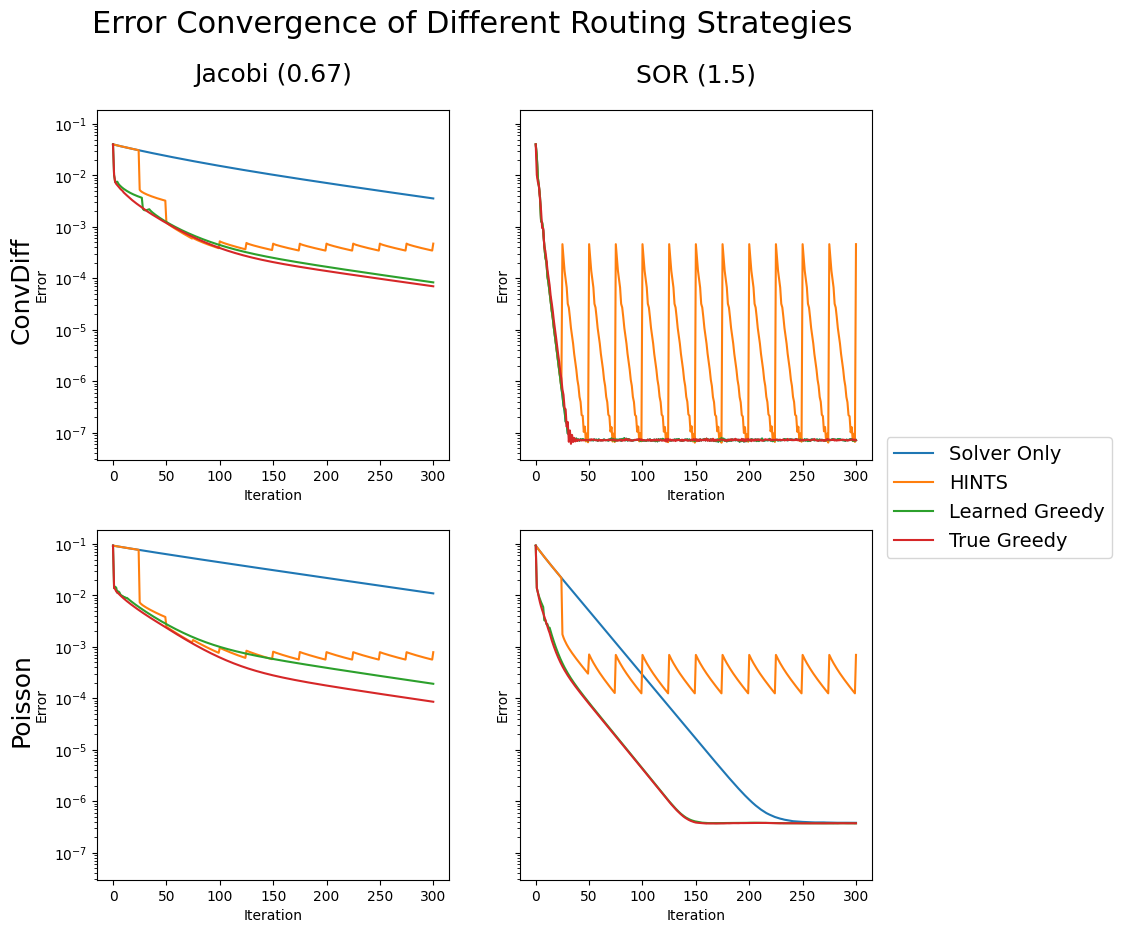
\includegraphics[width=0.55\linewidth]{neurips_images/sample_error_convergence_2.png}
    \caption{Convergence histories for representative test instances. Rows: ConvDiff (top) and Poisson (bottom). Columns: Jacobi (0.67) and Successive Over-relaxation (1.5). Greedy yields near-monotone decay and the lowest errors, whereas HINTS shows sawtooth behaviors.}
    \label{fig:errorcomparison2}
\end{figure}

\subsection{Prediction and Error Visualizations} \label{sec:error_viz}

\Cref{fig:prediction_visualization,fig:prediction_visualization2} provide qualitative visualizations of sample predictions across routing strategies and numerical solvers for both equations. While these prediction may appear identical to the ground truth, \Cref{fig:error_viz,fig:error_viz_2} reveals distinct error patterns with varying magnitudes across all predictions. In particular, our learned method consistently achieves the lower-magnitude errors compared to its respective baselines.

\begin{figure}[H]
    \centering
    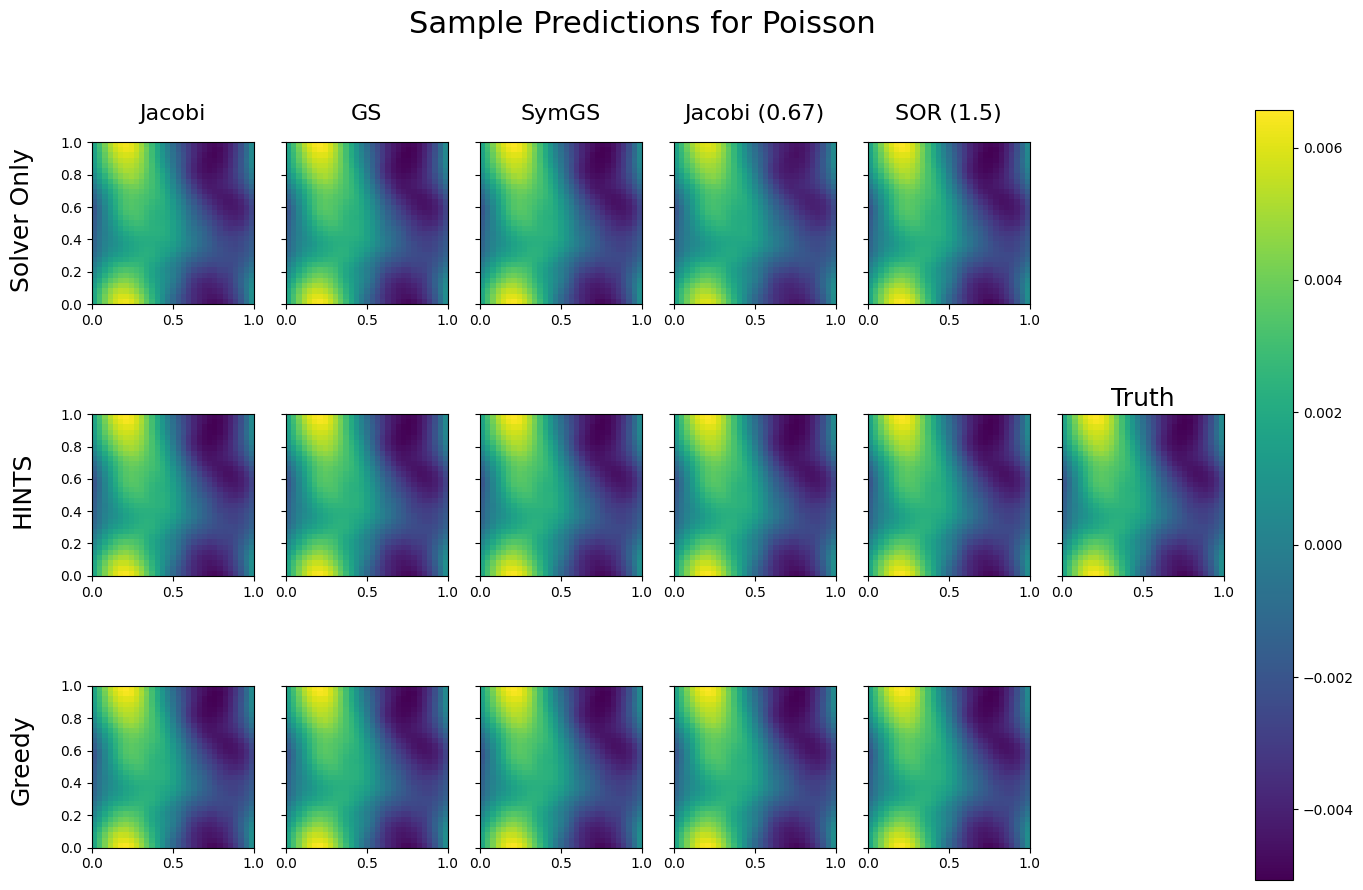
\includegraphics[width=0.55\linewidth]{neurips_images/prediction_poisson.png}
    \caption{Sample predictions for the Poisson equation across different solver pairings. Each column corresponds to a numerical solver (Jacobi, Gauss–Seidel (GS), Symmetric GS, Damped Jacobi, and Successive Over-relaxation), while rows show predictions from the corresponding solver-only baseline (top), HINTS (middle), and the learned greedy router (bottom). The ground truth solution is shown on the right.}
    \label{fig:prediction_visualization}
\end{figure}
\begin{figure}[H]
    \centering
    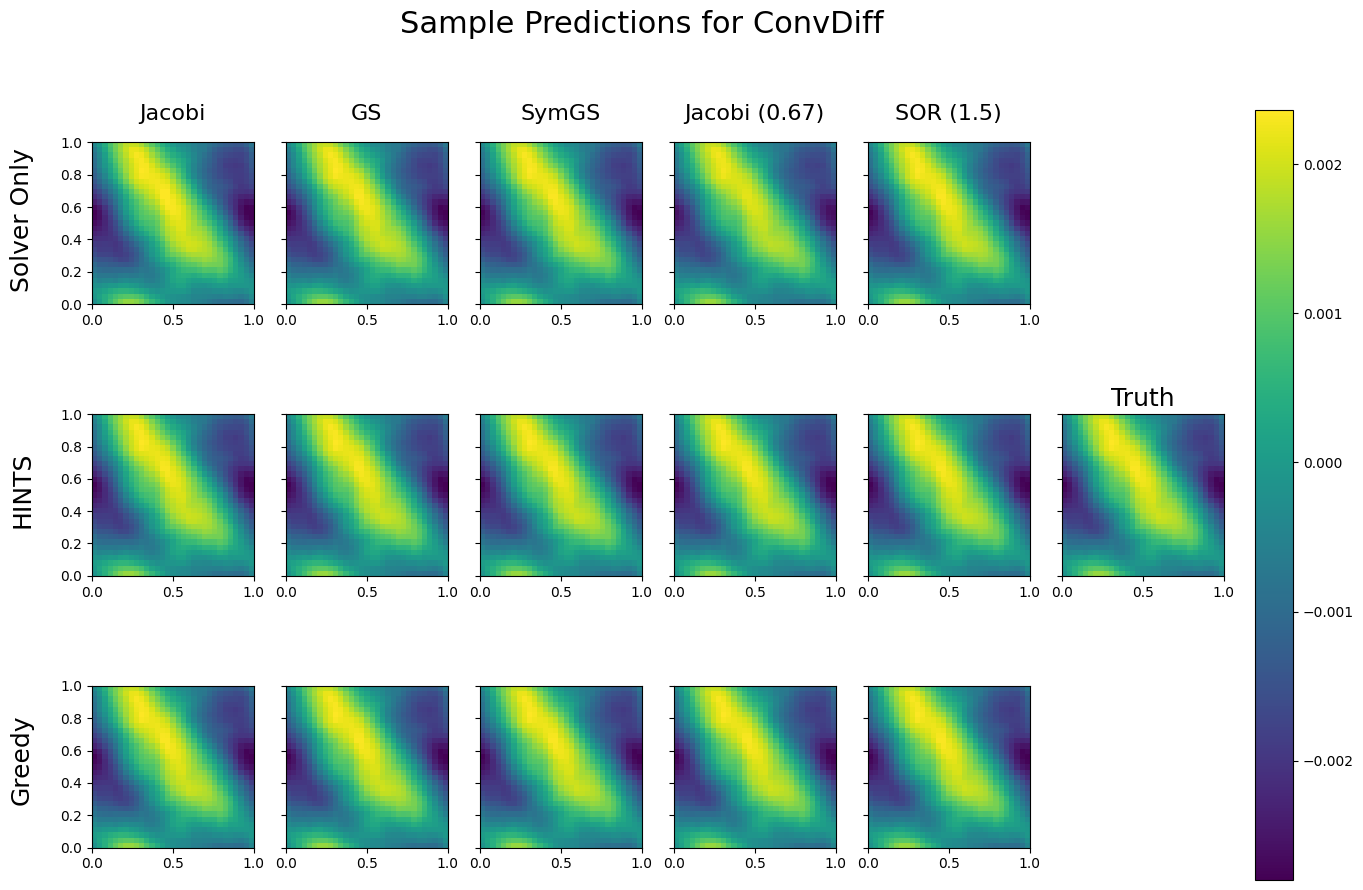
\includegraphics[width=0.55\linewidth]{neurips_images/prediction_convdiff.png}
    \caption{Sample predictions for the convection diffusion equation across different solver pairings. Each column corresponds to a numerical solver (Jacobi, Gauss–Seidel (GS), Symmetric GS, Damped Jacobi, and Successive Over-relaxation), while rows show predictions from the corresponding solver-only baseline (top), HINTS (middle), and the learned greedy router (bottom). The ground truth solution is shown on the right.}
    \label{fig:prediction_visualization2}
\end{figure}
\begin{figure}[H]
    \centering
    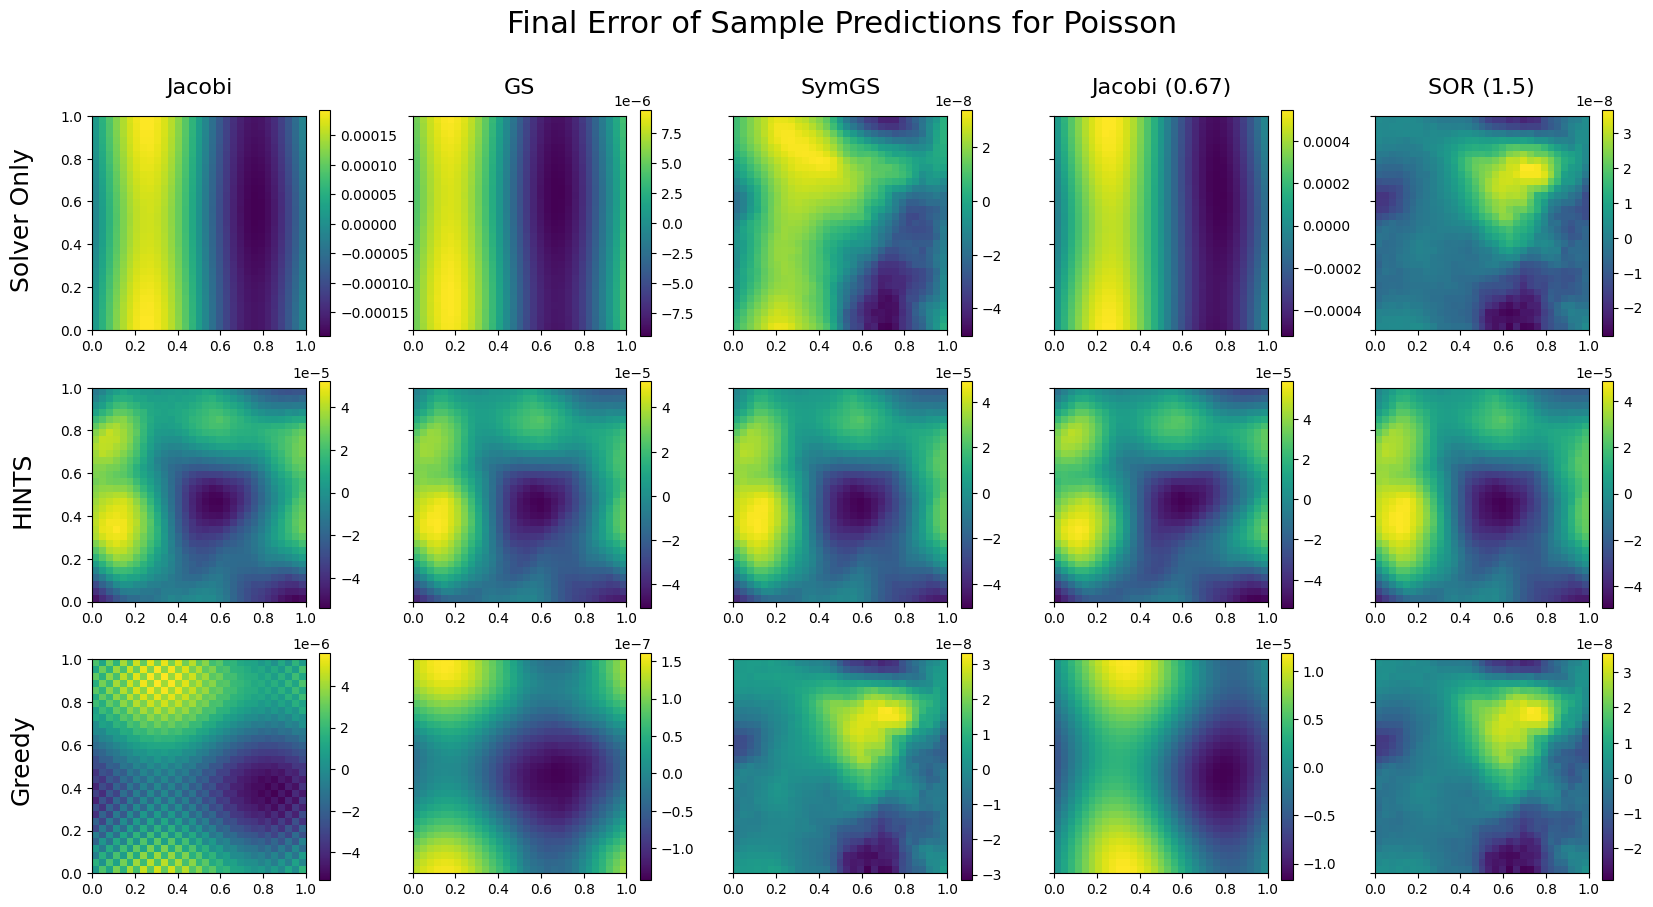
\includegraphics[width=0.55\linewidth]{neurips_images/error_viz_poisson.png}
    \caption{Pointwise error maps for Poisson sample predictions across solver families. Columns correspond to different numerical solvers, while rows show solver-only (top), HINTS (middle), and learned greedy router (bottom). Errors are computed as $u_h - u_h^{(T)} = e_h^{(T)}$. The learned greedy router consistently yields lower-magnitude errors compared to both solver-only and HINTS baselines.}
    \label{fig:error_viz}
\end{figure}
\begin{figure}[H]
    \centering
    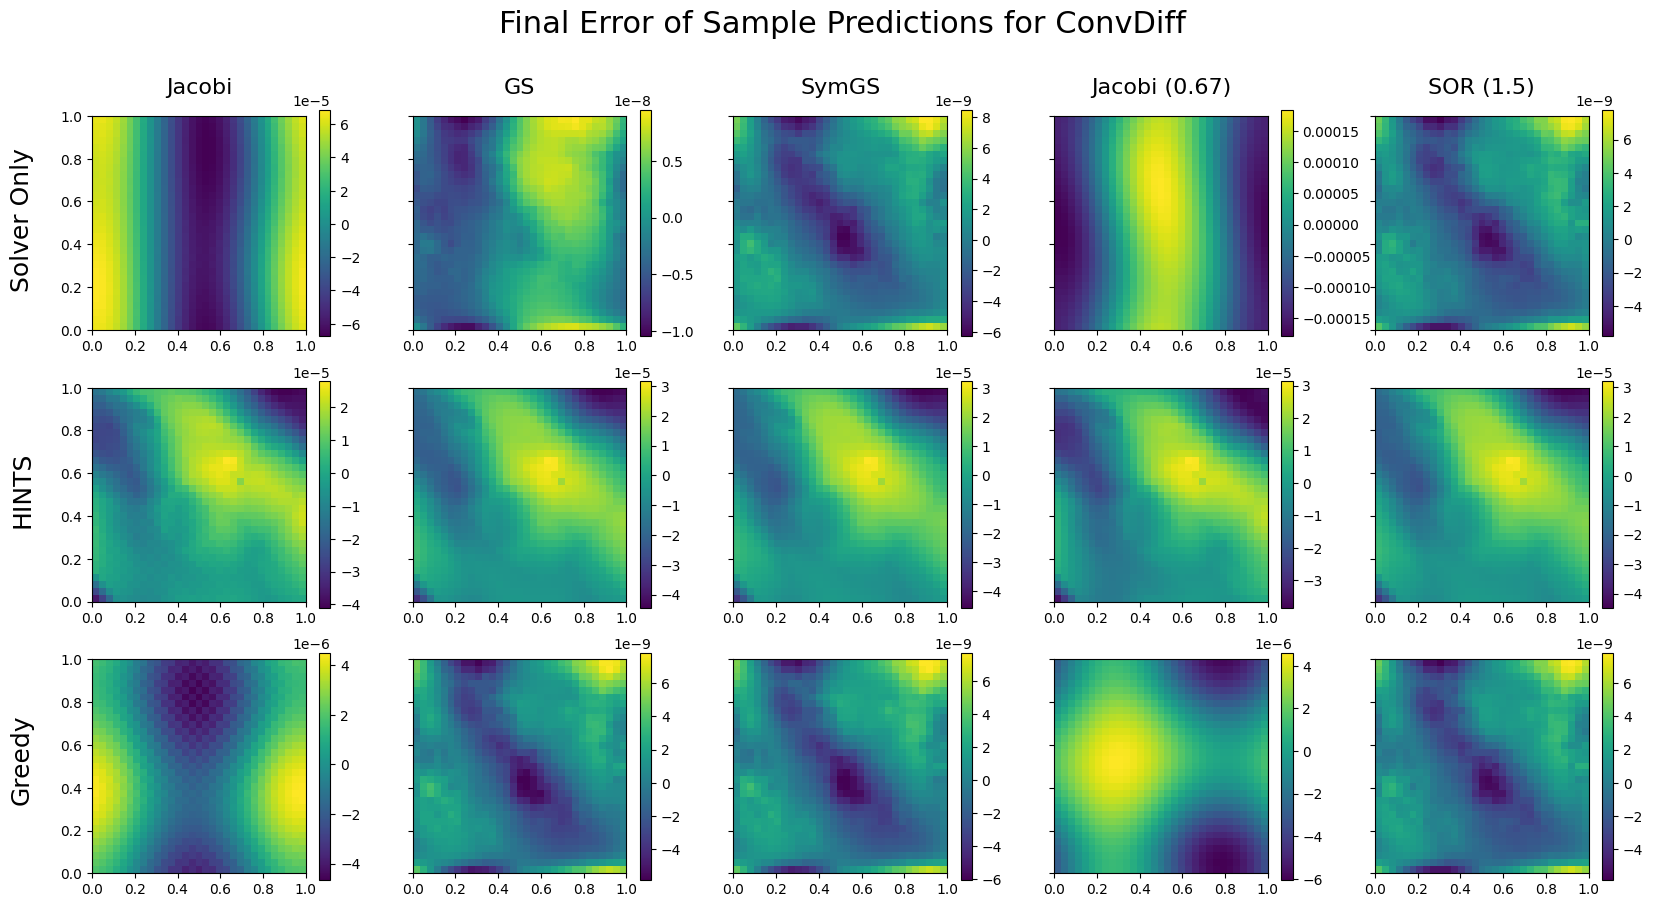
\includegraphics[width=0.55\linewidth]{neurips_images/error_viz_convdiff.png}
    \caption{Pointwise error maps for convection diffusion sample predictions across solver families. Columns correspond to different numerical solvers, while rows show solver-only (top), HINTS (middle), and learned greedy router (bottom). Errors are computed as $u_h - u_h^{(T)} = e_h^{(T)}$. The learned greedy router consistently yields lower-magnitude errors compared to both solver-only and HINTS baselines.}
    \label{fig:error_viz_2}
\end{figure}
\subsection{Residual Comparison} \label{sec:residualcomparison}


\begin{table}[H]
    \centering
    \caption{Final residual $\|\mathcal{L}_h^a e_h^{(T)}\|$ and AUC of residuals over iterations (lower is better). Values are reported as mean ($\pm$ standard error (s.e.)) over 128 test instances; residuals are scaled by $\times 10^{-3}$. If the residual norm is reported as $< 10^{-3}$, the corresponding raw value is $< 10^{-6}$. Statistical significance is evaluated via paired $t$-tests comparing each baseline (single-solver only and HINTS) to the learned greedy router under a one-sided alternative hypothesis that the learned router achieves lower residual and AUC. Reported $p$-values correspond to these tests.}
    \resizebox{\textwidth}{!}{
    \begin{tabular}{ccccccccc}
\hline \hline
         Equation &  \multicolumn{4}{c}{Poisson} & \multicolumn{4}{c}{ConvDiff} \\
         \hline 
         Methods & $\|\mathcal{L}_h^ae^{(T)}_h\| \times 10^{3}$ & $\|\mathcal{L}_h^ae^{(T)}_h\|$ $p$-value & AUC & AUC $p$-value & $\|\mathcal{L}_h^ae^{(T)}_h\| \times 10^{3}$ & $\|\mathcal{L}_h^ae^{(T)}_h\|$ $p$-value & AUC & AUC $p$-value\\
         \hline
         \multicolumn{9}{c}{Jacobi-related solvers}\\
         \hline
Jacobi only & 23.939 (66.755) & 0.021 & 43.475 (109.764) & $<10^{-3}$ & 27.208 (74.555) & 0.012 & 45.523 (114.774) & $<10^{-3}$ \\
HINTS-Jacobi & 193.327 (37.362) & $<10^{-3}$ & 39.763 (70.671) & $<10^{-3}$ & 266.421 (34.699) & $<10^{-3}$ & 42.851 (70.748) & $<10^{-3}$ \\
Learned Greedy-Jacobi & 20.870 (62.246) & - & 32.041 (83.647) & - & 20.786 (66.511) & - & 34.844 (84.666) & - \\
\hline
         \multicolumn{9}{c}{GS-related solvers}\\
         \hline
GS only & 0.761 (2.043) & $<10^{-3}$ & 20.776 (52.270) & $<10^{-3}$ & 0.002 (0.005) & $<10^{-3}$ & 10.720 (26.892) & $<10^{-3}$ \\
HINTS-GS & 183.359 (0.000) & $<10^{-3}$ & 22.581 (27.984) & $<10^{-3}$ & 246.877 (0.000) & $<10^{-3}$ & 18.654 (19.201) & $<10^{-3}$ \\
Learned Greedy-GS & 0.092 (0.145) & - & 11.960 (27.863) & - & 0.001 (0.003) & - & 7.322 (16.968) & - \\
\hline
         \multicolumn{9}{c}{SymGS-related solvers}\\
         \hline
SymGS only & 0.004 (0.009) & $<10^{-3}$ & 10.343 (25.957) & $<10^{-3}$ & 0.002 (0.004) & 0.004 & 8.604 (21.776) & $<10^{-3}$ \\
HINTS-SymGS & 185.601 (0.001) & $<10^{-3}$ & 15.489 (18.255) & $<10^{-3}$ & 245.629 (0.000) & $<10^{-3}$ & 16.515 (15.990) & $<10^{-3}$ \\
Learned Greedy-SymGS & 0.002 (0.005) & - & 7.149 (18.364) & - & 0.001 (0.002) & - & 6.481 (13.190) & -\\
\hline
         \multicolumn{9}{c}{Jacobi (0.67) -related solvers}\\
         \hline
Jacobi (0.67) only & 42.246 (112.968) & $<10^{-3}$ & 55.250 (138.258) & $<10^{-3}$ & 45.451 (121.431) & $<10^{-3}$ & 56.747 (141.901) & $<10^{-3}$ \\
HINTS-Jacobi (0.67) & 188.719 (0.008) & $<10^{-3}$ & 38.970 (53.035) & $<10^{-3}$ & 256.407 (0.005) & $<10^{-3}$ & 39.604 (52.578) & $<10^{-3}$ \\
Learned Greedy-Jacobi (0.67) & 9.290 (26.109) & - & 35.905 (86.881) & - & 9.010 (13.426) & - & 32.516 (83.488) & - \\
\hline
         \multicolumn{9}{c}{SOR (1.5)-related solvers}\\
         \hline
 SOR (1.5) only & 0.003 (0.008) & 0.5 & 9.044 (22.962) & $<10^{-3}$ & 0.002 (0.004) & 0.189 & 2.817 (7.499) & $<10^{-3}$ \\
HINTS-SOR (1.5) & 188.187 (0.001) & $<10^{-3}$ & 15.894 (19.565) & $<10^{-3}$ & 248.226 (0.001) & $<10^{-3}$ & 11.420 (7.498) & $<10^{-3}$ \\
Learned Greedy-SOR (1.5) & 0.003 (0.008) & - & 7.784 (19.939) & - & 0.002 (0.004) &  - & 5.530 (19.679) & - \\
\bottomrule
\end{tabular}}
    \label{tab:residualcomparison}
\end{table}

% \Comment{needs to be changed}
\begin{table}[H]
    \centering
    \caption{Final residual and AUC of squared $L^2$ residual for varying numbers of solvers. Values are mean ($\pm$ standard error (s.e.)) over 128 test instances; both mean and s.e. are reported in $\times 10^{-3}$.}
    \resizebox{\textwidth}{!}{
    \begin{tabular}{lcccc}
        \hline
          Equation & \multicolumn{2}{c}{Poisson} & \multicolumn{2}{c}{ConvDiff}\\
         \hline 
        $\mathcal{W}$ & $\|\mathcal{L}_h^ae^{(T)}_h\|$ & AUC & $\|\mathcal{L}_h^ae^{(T)}_h\|$ & AUC \\
         \hline
        $\{\text{Jacobi, GS}\}$ & 0.135 (0.096) & 11.815 (33.768) & 0.023 (0.044) & 5.765 (14.581) \\
        $\{\text{Jacobi, GS, SymGS}\}$ & 0.002 (0.004) & 5.118 (12.920) & 0.002 (0.002) & 4.810 (11.264) \\
        $\{\text{Jacobi, GS, SymGS, Jacobi (0.67)}\}$ & 0.013 (0.011) & 6.120 (14.651) & 0.010 (0.013) & 4.859 (11.473) \\
        $\{\text{Jacobi, GS, SymGS, Jacobi (0.67), SOR (1.5)}\}$  & 0.004 (0.006) & 8.196 (22.516) & 0.001 (0.002) & 3.209 (8.676) \\
         \hline
    \end{tabular}
    }
    \label{tab:residualcomparison2}
\end{table}


\Cref{tab:residualcomparison} summarizes the performance of single-solver schedules, HINTS, and greedy with respect to the final residuals $r_h^{(T)} =\|f_h - \mathcal{L}_h^a u_h^{(T)}\|$ or $\|\mathcal{L}_h^a e_h^{(T)}\|$ and its AUC $AUC_T = \sum_{t = 1}^T\|r^{(t)}_h\|^2_2$ . Greedy outperforms its HINTS and single-solver counterparts in most equations. We must note that our greedy router is trained to reduce error, not residual. The same error can induce very different residuals depending on the spectrum $\mathcal{L}_h^a$. \Cref{tab:residualcomparison2} exhibits how residuals are affected by the number of solvers in the solver ensemble. Similar to error, we observe both the final residual and AUC decrease as the number of solvers increase.



\subsection{Fourier mode-wise error comparison} \label{sec:fouriermodeerrorcomparison}

We assess frequency-resolved performance by projecting the error onto the discrete Fourier basis. \Cref{tab:modecomparison} report, for modes 1, 5, and 10, the mode-wise final error and mode-wise AUC, comparing single-solver baselines, HINTS, and the greedy router. As a result of including a deep learning model,Greedy consistently achieves the smallest mode-1 error/AUC across equations and solver families. For modes 5 and 10, single-solver schedules sometimes have an edge, reflecting the tendency of classical smoothers to damp high-frequency components more aggressively than ML surrogates (spectral bias). Overall, greedy delivers more uniform convergence across the spectrum: it routes to whichever solver most decreases the full $L^2$ error, and by Parseval’s identity $|e_h^{(t)}|_2^2=\sum_m|\hat u_m^{(t)}-\hat u_m|^2$, reductions in the objective correspond to reducing energy across all modes rather than giving preferential treatment to a subset. Additionally, in \Cref{tab:modecomparison2}, we observe that all mode-wise errors/AUCs reduce with the inclusion of more solvers.

% \begin{table}[H]
%     \centering
%         \caption{Caption}
%     \resizebox{\textwidth}{!}{
%     \begin{tabular}{ccccccccccccc}
% \hline \hline
% & \multicolumn{4}{|c|}{Mode 1} & \multicolumn{4}{|c|}{Mode 5} & \multicolumn{4}{|c|}{Mode 10}\\
% \hline 
%  Method & Final Error & Final Error p val & AUC & AUC p val & Final Error & Final Error p val & AUC & AUC p val & Final Error & Final Error p val & AUC & AUC p val \\
%  \hline
% Jacobi only & 0.135 (0.295) & 0.001 & 3.231 (7.056) & 0.001 & $<10^{-3}$ & 0.854 & 0.003 (0.010) & 0.996 & $<10^{-3}$ & 0.43 & 0.000 (0.001) & 0.999 \\
% HINTS-Jacobi & 5.730 (0.240) & 0.0 & 2.734 (3.371) & 0.0 & 0.028 (0.002) & 0.0 & 0.004 (0.012) & 0.989 & 0.006 (0.000) & 0.0 & 0.000 (0.001) & 0.993 \\
% Learned Greedy-Jacobi & 0.032 (0.085) & - & 0.841 (2.081) & - & $<10^{-3}$ & - & 0.009 (0.028) & - & $<10^{-3}$ & - & 0.001 (0.003) & - \\
% GS only& 0.002 (0.004) & 0.011 & 1.695 (3.702) & 0.001 & $<10^{-3}$ & 0.229 & 0.003 (0.011) & 0.995 & $<10^{-3}$ & 0.034 & 0.000 (0.001) & 0.998 \\
% HINTS-GS & 5.377 (0.000) & 0.0 & 2.113 (2.498) & 0.0 & 0.027 (0.000) & 0.0 & 0.005 (0.012) & 0.983 & 0.007 (0.000) & 0.0 & 0.000 (0.001) & 0.954 \\
% Learned Greedy-GS & 0.000 (0.001) & - & 0.465 (1.125) & - & $<10^{-3}$ & - & 0.009 (0.029) & - & $<10^{-3}$ & - & 0.001 (0.002) & - \\
% SymGS only & $<10^{-3}$ & 0.371 & 0.883 (1.919) & 0.003 & $<10^{-3}$ & 0.966 & 0.002 (0.006) & 0.975 & $<10^{-3}$ & 0.597 & 0.000 (0.001) & 0.968 \\
% HINTS-SymGS & 5.085 (0.000) & 0.0 & 1.432 (1.700) & 0.0 & 0.025 (0.000) & 0.0 & 0.002 (0.007) & 0.958 & 0.007 (0.000) & 0.0 & 0.000 (0.001) & 0.885 \\
% Learned Greedy-SymGS & $<10^{-3}$ & - & 0.334 (0.943) & - & $<10^{-3}$ & - & 0.007 (0.025) & - & $<10^{-3}$ & - & 0.001 (0.002) & - \\
% only Jacobi (0.67) & 1.063 (2.321) & 0.004 & 4.771 (10.421) & 0.004 & $<10^{-3}$ & 0.262 & 0.005 (0.017) & 0.987 & $<10^{-3}$ & 0.89 & $<10^{-3}$ & 0.999 \\
% HINTS-Jacobi (0.67) & 5.804 (0.001) & 0.0 & 2.983 (3.666) & 0.018 & 0.029 (0.000) & 0.0 & 0.007 (0.019) & 0.975 & 0.006 (0.000) & 0.0 & $<10^{-3}$ & 0.997 \\
% Learned Greedy-Jacobi (0.67) & 0.390 (1.195) & - & 1.804 (5.363) & - & $<10^{-3}$ & - & 0.017 (0.058) & - & $<10^{-3}$ & - & 0.001 (0.002) & - \\
% only SOR (1.5) & $<10^{-3}$ & 0.852 & 0.727 (1.594) & 0.001 & $<10^{-3}$ & 0.254 & 0.005 (0.019) & 0.996 & $<10^{-3}$ & 0.9 & 0.001 (0.002) & 0.997 \\
% HINTS-SOR (1.5) & 4.826 (0.000) & 0.0 & 1.239 (1.484) & 0.0 & 0.027 (0.000) & 0.0 & 0.007 (0.020) & 0.978 & 0.008 (0.000) & 0.0 & 0.001 (0.002) & 0.345 \\
% Learned Greedy-SOR (1.5) & $<10^{-3}$ & - & 0.302 (0.757) & - & $<10^{-3}$ & - & 0.010 (0.032) & - & $<10^{-3}$ & - & 0.001 (0.003) & - \\

% \hline \hline
% \end{tabular}
%     }

%     \label{tab:modecomparisonpoisson}
% \end{table}

\begin{table}[H]
    \centering
      \caption{Final error and AUC of squared $L^2$ error for Mode 1, 5, and 10 (lower is better) for Poisson and ConvDiff. Values are mean ($\pm$ standard error (s.e.)) over 128 test instances; both mean and s.e. of final errors are reported in $\times 10^{-3}$.  If the residual norm is reported as $< 10^{-3}$, the corresponding raw value is $< 10^{-6}$.}
    \resizebox{\textwidth}{!}{
    \begin{tabular}{ccccccccccccc}
\hline \hline
& \multicolumn{6}{c}{Poisson} & \multicolumn{6}{c}{ConvDiff} \\
& \multicolumn{2}{c}{Mode 1} & \multicolumn{2}{c}{Mode 5} & \multicolumn{2}{c}{Mode 10} & \multicolumn{2}{c}{Mode 1} & \multicolumn{2}{c}{Mode 5} & \multicolumn{2}{c}{Mode 10}\\
\hline 
 Method & Final Error &  AUC &  Final Error &  AUC &  Final Error &  AUC & Final Error &  AUC &  Final Error &  AUC &  Final Error &  AUC \\
 \hline
 \multicolumn{13}{c}{Jacobi-related solvers}\\
 \hline
Jacobi Only&0.135 (0.295) & 3.231 (7.056) & $<10^{-3}$ & 0.003 (0.010) & $<10^{-3}$ & 0.000 (0.001) & 0.079 (0.171) & 1.084 (2.369) & $<10^{-3}$ & 0.003 (0.011) & $<10^{-3}$ & 0.000 (0.001) \\
HINTS-Jacobi & 5.730 (0.240) & 2.734 (3.371) & 0.028 (0.002) & 0.004 (0.012) & 0.006 (0.000) & 0.000 (0.001) & 0.994 (0.220) & 0.697 (1.091) & 0.061 (0.001) & 0.005 (0.012) & 0.022 (0.001) & 0.001 (0.001) \\
Learned Greedy-Jacobi & 0.032 (0.085) & 0.841 (2.081) & $<10^{-3}$ & 0.009 (0.028) & $<10^{-3}$ & 0.001 (0.003) & 0.021 (0.055) & 0.324 (0.780) & $<10^{-3}$ & 0.009 (0.025) & $<10^{-3}$ & 0.001 (0.002) \\
 \hline
 \multicolumn{13}{c}{GS-related solvers}\\
 \hline
GS Only & 0.002 (0.004) & 1.695 (3.702) & $<10^{-3}$ & 0.003 (0.011) & $<10^{-3}$ & 0.000 (0.001) & $<10^{-3}$ & 0.205 (0.452) & $<10^{-3}$ & 0.002 (0.006) & $<10^{-3}$ & $<10^{-3}$ \\
HINTS-GS & 5.377 (0.000) & 2.113 (2.498) & 0.027 (0.000) & 0.005 (0.012) & 0.007 (0.000) & 0.000 (0.001) & 0.661 (0.000) & 0.271 (0.432) & 0.065 (0.000) & 0.003 (0.006) & 0.019 (0.000) & $<10^{-3}$ \\
Learned Greedy-GS & 0.000 (0.001) & 0.465 (1.125) & $<10^{-3}$ & 0.009 (0.029) & $<10^{-3}$ & 0.001 (0.002) & $<10^{-3}$ & 0.075 (0.151) & $<10^{-3}$ & 0.005 (0.017) & $<10^{-3}$ & 0.001 (0.001) \\
 \hline
 \multicolumn{13}{c}{SymGS-related solvers}\\
 \hline
SymGS Only& $<10^{-3}$ & 0.883 (1.919) & $<10^{-3}$ & 0.002 (0.006) & $<10^{-3}$ & 0.000 (0.001) & $<10^{-3}$ & 0.180 (0.400) & $<10^{-3}$ & 0.001 (0.005) & $<10^{-3}$ & 0.000 (0.001) \\
HINTS-SymGS & 5.085 (0.000) & 1.432 (1.700) & 0.025 (0.000) & 0.002 (0.007) & 0.007 (0.000) & 0.000 (0.001) & 0.672 (0.000) & 0.240 (0.381) & 0.070 (0.000) & 0.002 (0.005) & 0.019 (0.000) & 0.000 (0.001) \\
Learned Greedy-SymGS & $<10^{-3}$ & 0.334 (0.943) & $<10^{-3}$ & 0.007 (0.025) & $<10^{-3}$ & 0.001 (0.002) & $<10^{-3}$ & 0.079 (0.193) & $<10^{-3}$ & 0.004 (0.012) & $<10^{-3}$ & 0.001 (0.001) \\
 \hline
 \multicolumn{13}{c}{Jacobi (0.67)-related solvers}\\
 \hline
Jacobi (0.67) Only& 1.063 (2.321) & 4.771 (10.421) & $<10^{-3}$ & 0.005 (0.017) & $<10^{-3}$ & $<10^{-3}$ & 0.428 (0.934) & 1.535 (3.352) & $<10^{-3}$ & 0.004 (0.016) & $<10^{-3}$ & $<10^{-3}$ \\
HINTS-Jacobi (0.67) & 5.804 (0.001) & 2.983 (3.666) & 0.029 (0.000) & 0.007 (0.019) & 0.006 (0.000) & $<10^{-3}$ & 1.080 (0.000) & 0.776 (1.158) & 0.065 (0.000) & 0.008 (0.017) & 0.021 (0.000) & $<10^{-3}$ \\
Learned Greedy-Jacobi (0.67) & 0.390 (1.195) & 1.804 (5.363) & $<10^{-3}$ & 0.017 (0.058) & $<10^{-3}$ & 0.001 (0.002) & 0.096 (0.208) & 0.435 (0.910) & $<10^{-3}$ & 0.013 (0.044) & $<10^{-3}$ & 0.001 (0.004) \\
 \hline
 \multicolumn{13}{c}{SOR (1.5) -related solvers}\\
 \hline
SOR (1.5) Only& $<10^{-3}$ & 0.727 (1.594) & $<10^{-3}$ & 0.005 (0.019) & $<10^{-3}$ & 0.001 (0.002) & $<10^{-3}$ & 0.037 (0.082) & $<10^{-3}$ & 0.002 (0.007) & $<10^{-3}$ & 0.000 (0.001) \\
HINTS-SOR (1.5) & 4.826 (0.000) & 1.239 (1.484) & 0.027 (0.000) & 0.007 (0.020) & 0.008 (0.000) & 0.001 (0.002) & 0.645 (0.000) & 0.080 (0.082) & 0.068 (0.000) & 0.005 (0.007) & 0.019 (0.000) & 0.001 (0.001) \\
Learned Greedy-SOR (1.5) & $<10^{-3}$ & 0.302 (0.757) & $<10^{-3}$ & 0.010 (0.032) & $<10^{-3}$ & 0.001 (0.003) & $<10^{-3}$ & 0.049 (0.119) & $<10^{-3}$ & 0.007 (0.030) & $<10^{-3}$ & 0.001 (0.002) \\
\bottomrule
\hline \hline
\end{tabular}
    }

    \label{tab:modecomparison}
\end{table}

% \begin{table}[H]
%     \centering
%     \resizebox{\textwidth}{!}{%
%     \begin{tabular}{|c|c|c|c|c|c|c|c|c|c|c|c|c|}
%         \hline
%          Equation & \multicolumn{6}{|c|}{1D Poisson} & \multicolumn{6}{|c|}{2D Poisson} \\
%         \hline
%          Methods/ Mode & Mode 1 Error & Mode 1 AUC & Mode 5 Error & Mode 5 AUC &Mode 10 Error &Mode 10 AUC & Mode 1 Error & Mode 1 AUC & Mode 5 Error & Mode 5 AUC &Mode 10 Error &Mode 10 AUC\\
%          \hline
%          \multicolumn{13}{|c|}{Jacobi-related Solvers} \\
%         \hline
%         Jacobi Only & 1.124 (0.612) & 732.713 (399.296) & -  & \textbf{0.076 (0.043)} & - & \textbf{0.001}  & 0.03 (0.014) & 382.094 (183.783) & \textbf{-} & \textbf{0.012 (0.006)} & \textbf{-} & \textbf{-}\\
%         HINTS-Jacobi & 0.059 (0.024) & 128.076 (64.871) & 0.001 (0.001) & 0.348 (0.121) & - & 0.041 (0.021) & 0.296 (0.003) & 227.594 (78.715) & 0.003 & 0.169 (0.055) & 0.001 & 0.03 (0.009) \\
%         Greedy-Jacobi & \textbf{0.006 (0.004)} & \textbf{4.152 (2.593)} & - & 0.192 (0.094) & - & 0.025 (0.016) & \textbf{0.009 (0.004)} & \textbf{114.046 (54.747)} & \textbf{-} & 0.105 (0.057) & \textbf{-} & 0.014 (0.008)\\
%         \hline
%         \multicolumn{13}{|c|}{GS-related Solvers} \\
%         \hline
%         GS Only & 0.285 (0.155) & 458.834 (250.064) & \textbf{-} & 0.223 (0.136) & - & 0.096 (0.072) & \textbf{-} & 196.347 (94.367) & - & 0.014 (0.007) & \textbf{-} & \textbf{0.001}\\
%         HINTS-GS & 0.017 & 100.582 (52.598) & 0.001 & 0.176 (0.049) & -  & 0.049 (0.028) & 0.258  & 168.877 (59.252) & 0.003 & 0.162 (0.032) & 0.001  & 0.052 (0.006)\\
%         Greedy-GS & \textbf{0.002 (0.001)} & \textbf{2.661 (1.595)} & \textbf{-} & \textbf{0.12 (0.058)} & - & \textbf{0.026 (0.015)} & \textbf{-} & \textbf{62.858 (30.237)} & - & \textbf{0.09 (0.044)} & \textbf{-} & 0.014 (0.007) \\
%          \hline
%          \multicolumn{13}{|c|}{Multigrid methods} \\
%          \hline
%         MG Only & 0.282 (0.078) & 116.885 (42.581) & - & 0.043 (0.022) & - & 0.013 (0.007) & 0.001  & 25.497 (11.766) & - & \textbf{0.003 (0.001)} & - & \textbf{-}\\
%         HINTS-MG & 0.014 & 43.405 (20.908) & - & \textbf{0.027 (0.006)} & - & 0.009 (0.003) & 0.078 & 31.289 (10.201) & - & 0.035 (0.004) & - & 0.01 (0.001)\\
%         Greedy-MG & \textbf{0.003 (0.002)} & \textbf{0.999 (0.622)} & - & 0.029 (0.013) & - & \textbf{0.008 (0.005)} & \textbf{-} & \textbf{13.358 (6.045)} & - & 0.031 (0.016) & - & 0.007 (0.004) \\
%          \hline
%     \end{tabular}
%     }
%     \caption{Final error and AUC of squared $L^2$ error for Mode 1, 5, and 10 (lower is better) for 1D/2D Poisson. Values are mean ($\pm$ standard error (s.e.)) over 64 test instances; both mean and s.e. are reported in $\times 10^{-3}$. If a standard error is not shown, it is $< 10^{-3}$ in the reported units (raw $< 10^{-6}$). Bold indicates the best method within each solver family.}
%     \label{tab:modecomparisonPoisson}
% \end{table}



\begin{table}[H]
    \centering
    \caption{Final error and AUC of squared $L^2$ error of Mode 1, 5, and 10 for varying numbers of solvers. Values are mean ($\pm$ standard error (s.e.)) over 128 test instances; both mean and s.e. are reported in $\times 10^{-3}$.}
    \resizebox{\textwidth}{!}{%
    \begin{tabular}{lcccccccccccc}
        \hline
         Equation & \multicolumn{6}{c}{Poisson} & \multicolumn{6}{c}{ConvDiff} \\
        \hline
         $\mathcal{W}$/ Mode & Mode 1 Error & Mode 1 AUC & Mode 5 Error & Mode 5 AUC &Mode 10 Error &Mode 10 AUC & Mode 1 Error & Mode 1 AUC & Mode 5 Error & Mode 5 AUC &Mode 10 Error &Mode 10 AUC\\
         \hline
         $\{\text{Jacobi, GS}\}$ & 0.000 (0.001) & 0.267 (0.571) & $<10^{-3}$ & 0.006 (0.023) & $<10^{-3}$ & 0.001 (0.003) & $<10^{-3}$ & 0.055 (0.112) & $<10^{-3}$ & 0.002 (0.008) & $<10^{-3}$ & 0.000 (0.002) \\
        $\{\text{Jacobi, GS, SymGS}\}$ & 0.000 (0.001) & 0.185 (0.413) & $<10^{-3}$ & 0.003 (0.009) & $<10^{-3}$ & 0.000 (0.002) & $<10^{-3}$ & 0.054 (0.114) & $<10^{-3}$ & 0.002 (0.007) & $<10^{-3}$ & 0.000 (0.001) \\
    $\{\text{Jacobi, GS, SymGS, Jacobi (0.67)}\}$ & 0.000 (0.001) & 0.172 (0.333) & $<10^{-3}$ & 0.003 (0.010) & $<10^{-3}$ & 0.000 (0.002) & $<10^{-3}$ & 0.056 (0.119) & $<10^{-3}$ & 0.002 (0.007) & $<10^{-3}$ & 0.000 (0.001) \\
    $\{\text{Jacobi, GS, SymGS, Jacobi (0.67), SOR (1.5)}\}$ & 0.000 (0.001) & 0.210 (0.399) & $<10^{-3}$ & 0.006 (0.023) & $<10^{-3}$ & 0.001 (0.004) & $<10^{-3}$ & 0.026 (0.061) & $<10^{-3}$ & 0.002 (0.005) & $<10^{-3}$ & 0.000 (0.002) \\
         \hline
    \end{tabular}
    }
    \label{tab:modecomparison2}
\end{table}


 
\clearpage
\subsection{Ensemble Solver Decisions and DeepONet Usage} \label{sec:solverdecisions}


\begin{figure}[H]
    \centering
    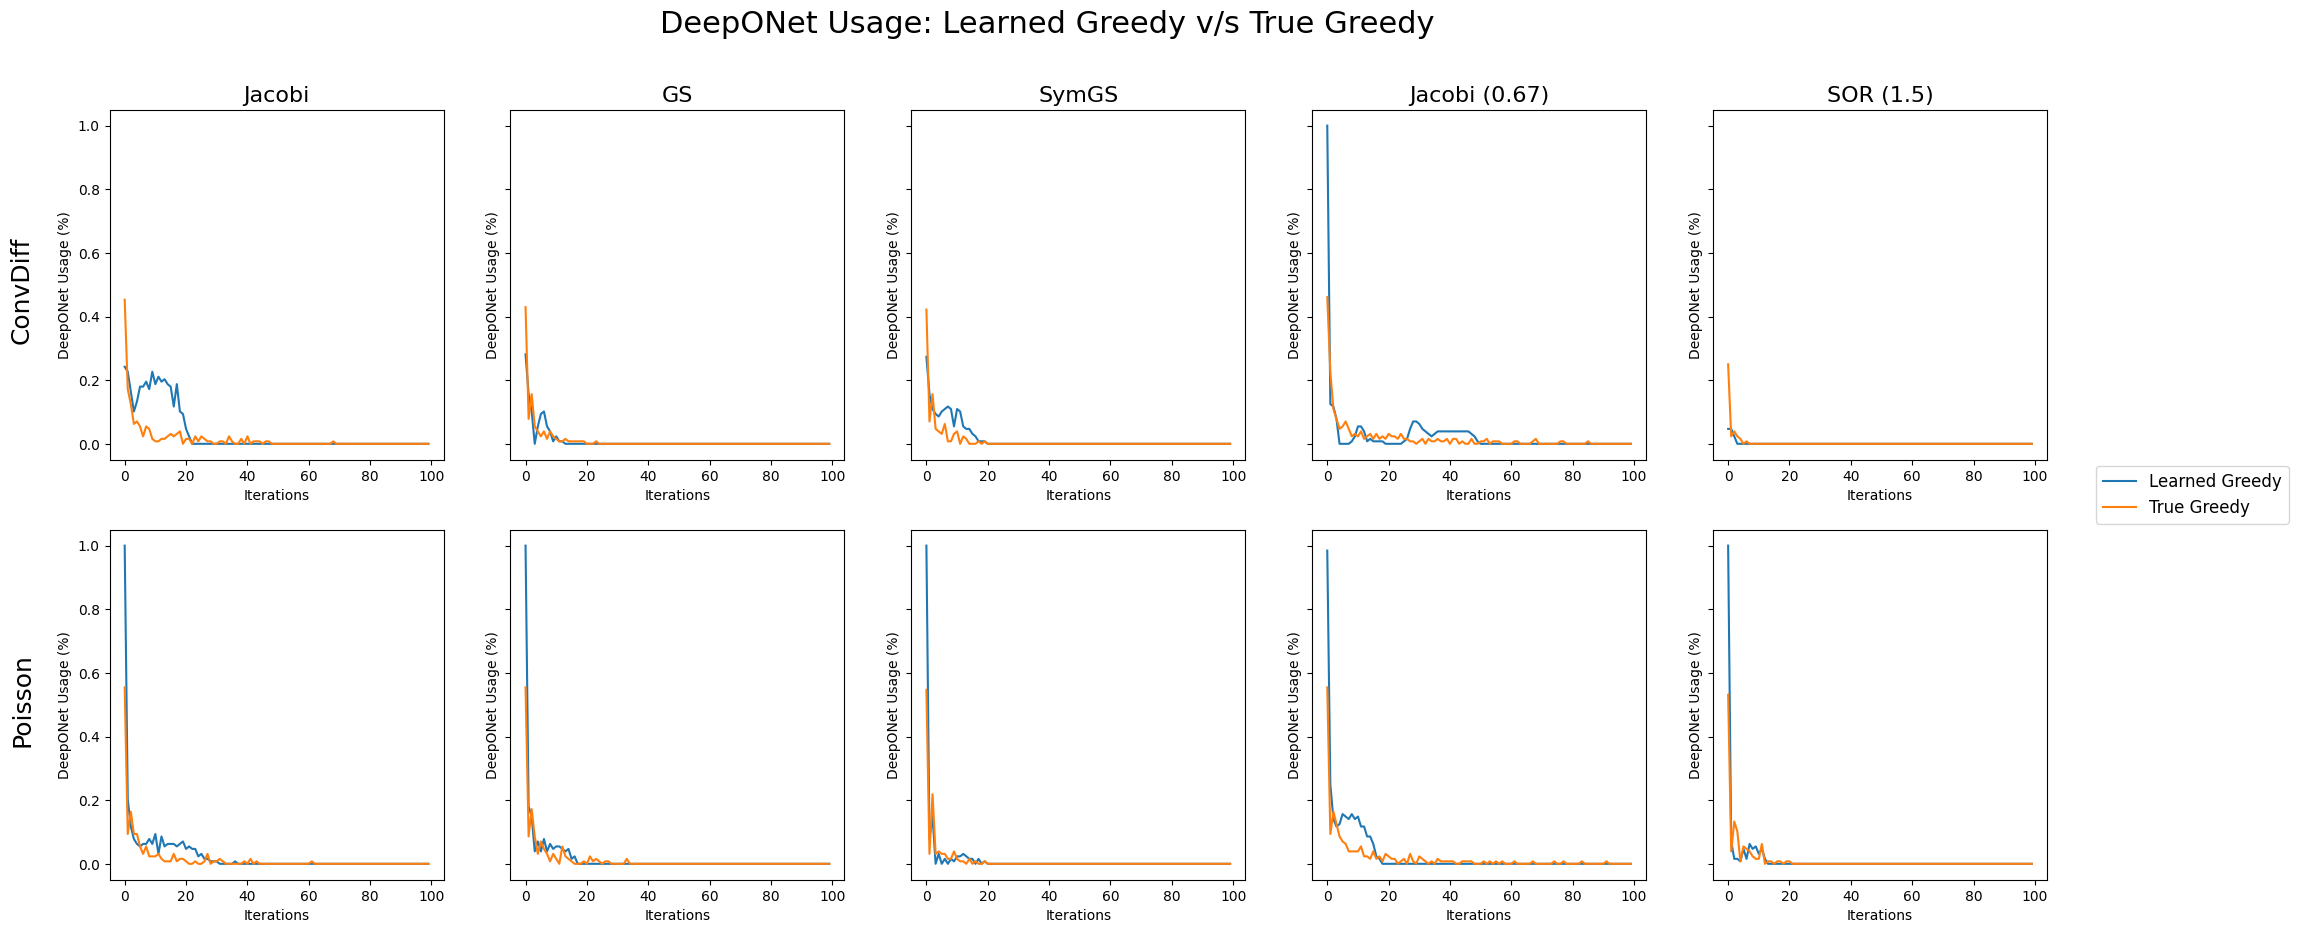
\includegraphics[width=1.0\linewidth]{neurips_images/deeponet_comparison_2.png}
    \caption{DeepONet usage over iterations for learned and true greedy routing across solver families. Columns correspond to different numerical solvers, and rows correspond to the two equations. The learned router closely follows the true greedy policy, capturing its nonuniform usage of DeepONet across iterations. For readability, we display the first 100 iterations (out of 300 total)}
    \label{fig:deeponet_usage}
\end{figure}
\begin{figure}[H]
    \centering
    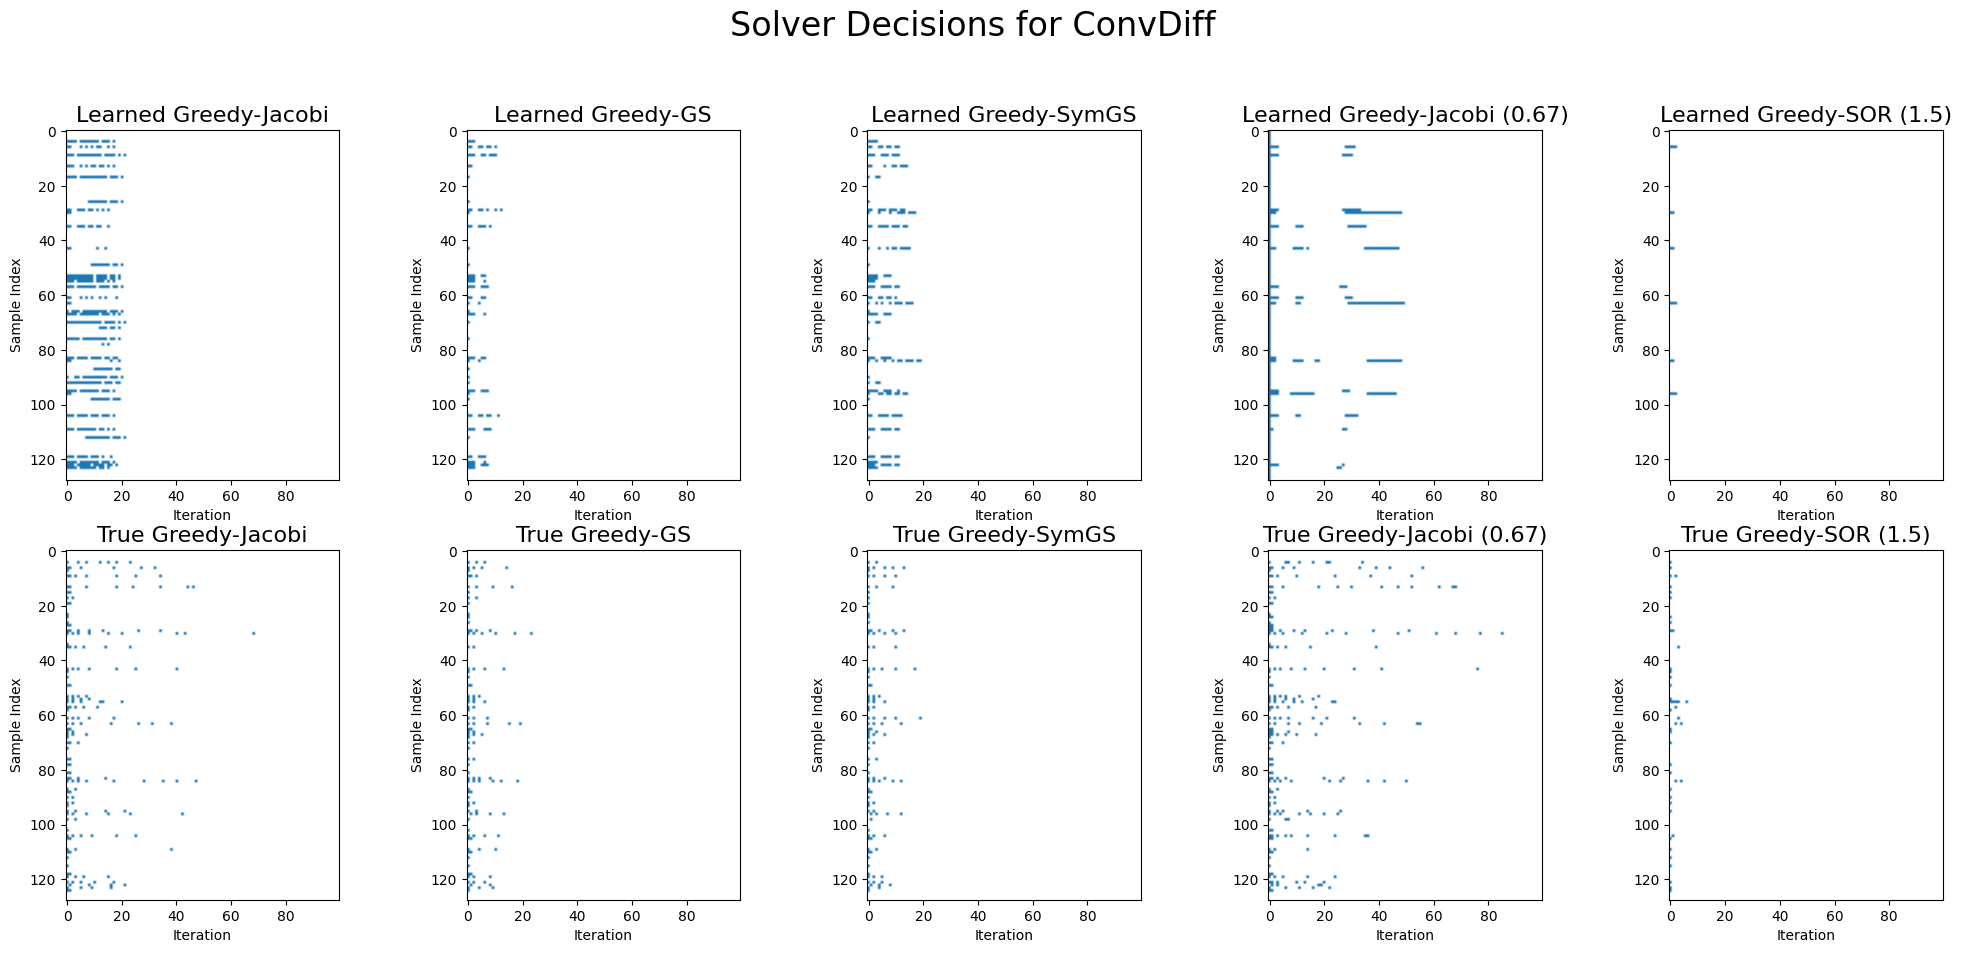
\includegraphics[width=1.0\linewidth]{neurips_images/solver_decisions_convdiff.png}
    \caption{Solver selection patterns for the convection–diffusion equation across different solver pairings and test samples. Each column corresponds to a solver family, while rows show decisions from the learned greedy router (top) and the true greedy policy (bottom). Colored entries indicate iterations where the neural operator is selected, with blank regions corresponding to numerical solver updates. The learned router exhibits instance-dependent routing behavior.}
    \label{fig:solver_decisions_convdiff}
\end{figure}

\begin{figure}[H]
    \centering
    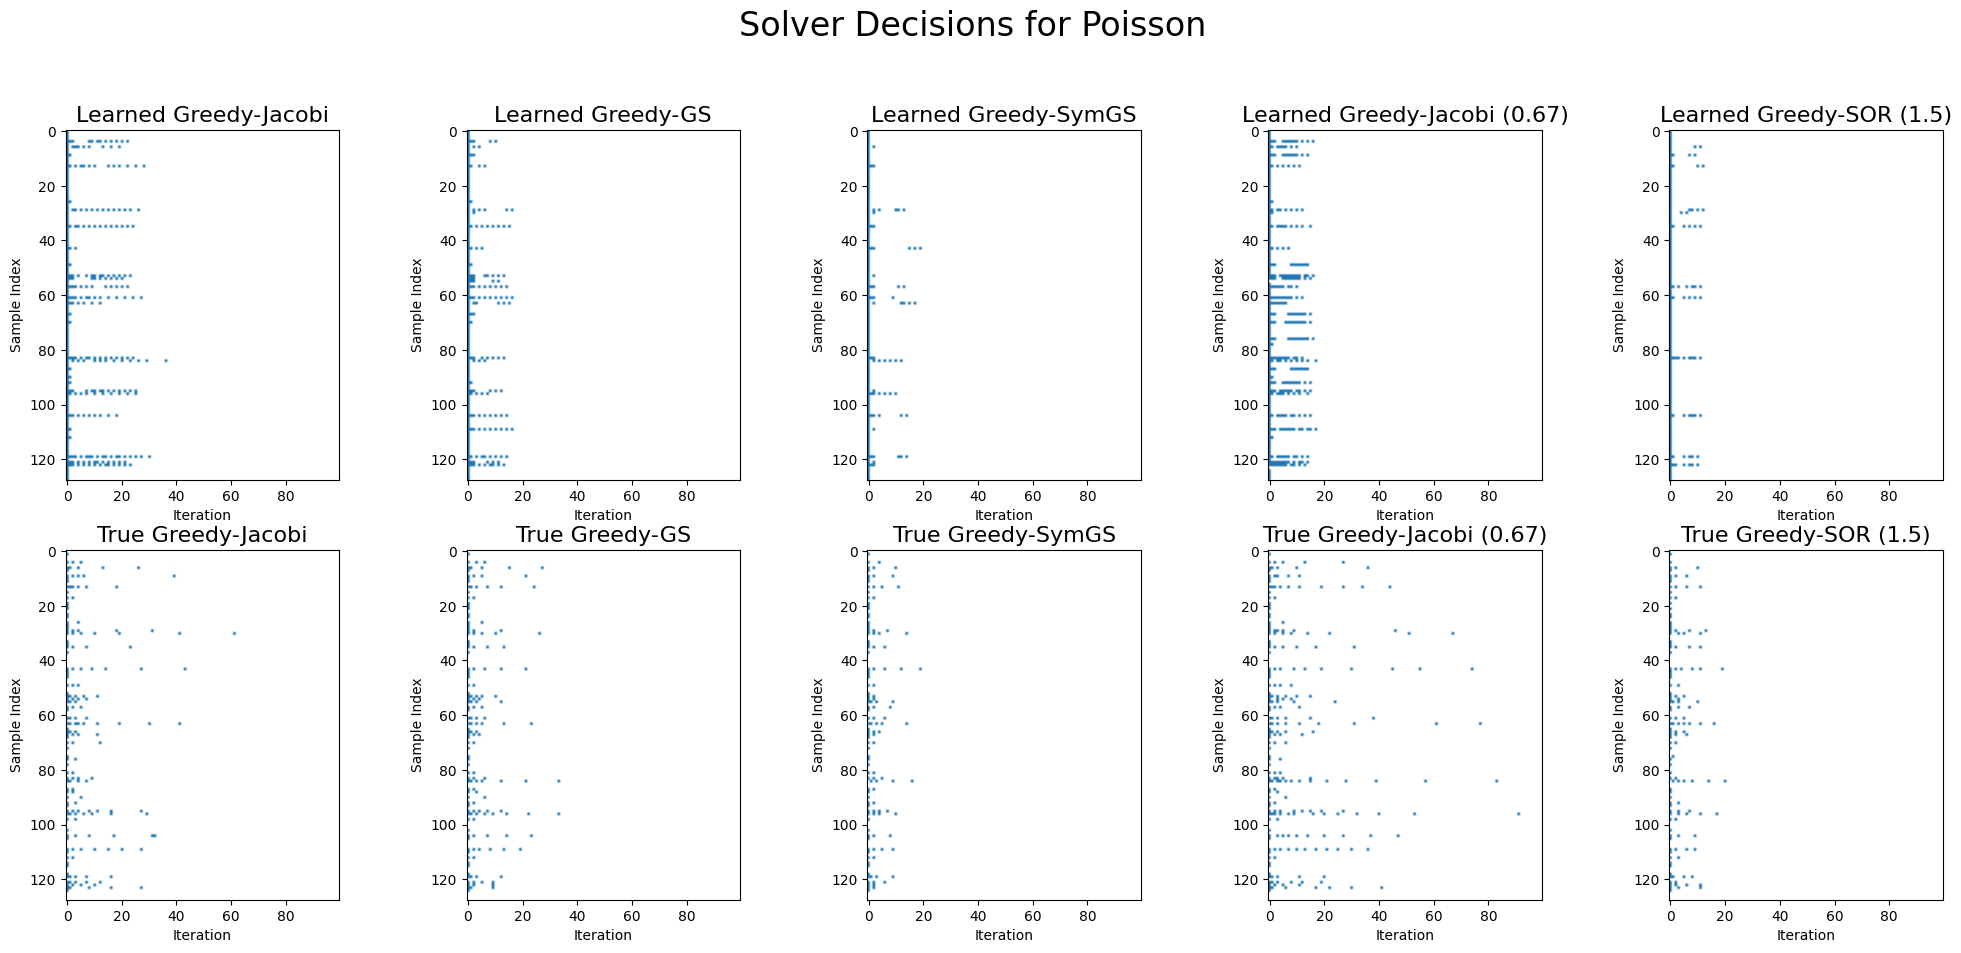
\includegraphics[width=1.0\linewidth]{neurips_images/solver_decisions_poisson.png}
    \caption{Solver selection patterns for the Poisson equation across different solver pairings and test samples. Each column corresponds to a solver family, while rows show decisions from the learned greedy router (top) and the true greedy policy (bottom). Colored entries indicate iterations where the neural operator is selected, with blank regions corresponding to numerical solver updates. The learned router exhibits instance-dependent routing behavior.}
    \label{fig:solver_decisions_poisson}
\end{figure}
\Cref{fig:deeponet_usage} highlights the proportion of DeepONet calls across iterations, while \Cref{fig:solver_decisions_convdiff,fig:solver_decisions_poisson} visualize the routing decisions of the learned and true greedy policies across all test samples and solver families.

Two key observations emerge. First, the routing strategy is highly sample-dependent, indicating that a fixed routing schedule across all instances would be suboptimal and can slow convergence. Second, the learned routing policy closely tracks the behavior of the true greedy policy, providing empirical support for the approximation guarantees discussed in \Cref{sec:approxgreedy}. In particular, the learned policy can be viewed as a smoothed approximation of the true greedy strategy, capturing its overall structure while exhibiting minor deviations due to learning and finite-sample effects.

\begin{table}[H]
\centering
\caption{
Average component selection frequencies for the Poisson equation.
Rows indicate the router access set. Entries are mean ($\pm$ s.e.) over 128 test instances.
Here $\mathrm{NO}$ denotes the neural operator; ``-'' indicates that the component is not available to the router.
}
\label{tab:multsolverpoisson}

\resizebox{\textwidth}{!}{
\begin{tabular}{lllllll}
\toprule
$\mathcal{W}$ & Jacobi & GS & SSOR & Jacobi (0.67) & SOR (1.5) & DeepONet \\
\midrule
$\{\text{Jacobi, GS}\}$ & 0.405 (0.143) & 0.588 (0.134) & - & - & - & 0.007 (0.011) \\
$\{\text{Jacobi, GS, SSOR}\}$ & 0.000 (0.000) & 0.000 (0.000) & 0.996 (0.005) & - & - & 0.004 (0.005) \\
$\{\text{Jacobi, GS, SSOR, Jacobi (0.67)}\}$ & 0.227 (0.112) & 0.212 (0.118) & 0.434 (0.212) & 0.121 (0.102) & - & 0.005 (0.007) \\
$\{\text{Jacobi, GS, SSOR, Jacobi (0.67), SOR (1.5)}\}$& 0.009 (0.033) & 0.570 (0.057) & 0.260 (0.040) & 0.000 (0.000) & 0.156 (0.013) & 0.005 (0.005) \\
\bottomrule
\end{tabular}
}
\end{table}

\begin{table}[H]
\centering
\caption{
Average component selection frequencies for the Convection-Diffusion equation.
Rows indicate the router access set. Entries are mean ($\pm$ s.e.) over 128 test instances.
Here $\mathrm{NO}$ denotes the neural operator; ``-'' indicates that the component is not available to the router.
}
\label{tab:multsolverconvdiff}

\resizebox{\textwidth}{!}{
\begin{tabular}{lllllll}
\toprule
$\mathcal{W}$ & Jacobi & GS & SSOR & Jacobi (0.67) & SOR (1.5) & DeepONet \\
\midrule
$\{\text{Jacobi, GS}\}$ & 0.417 (0.307) & 0.579 (0.307) & - & - & - & 0.004 (0.006) \\
$\{\text{Jacobi, GS, SSOR}\}$ & 0.109 (0.109) & 0.396 (0.110) & 0.493 (0.175) & - & - & 0.003 (0.005) \\
$\{\text{Jacobi, GS, SSOR, Jacobi (0.67)}\}$ &0.168 (0.096) & 0.190 (0.166) & 0.410 (0.227) & 0.229 (0.146) & - & 0.003 (0.004) \\
$\{\text{Jacobi, GS, SSOR, Jacobi (0.67), SOR (1.5)}\}$& 0.307 (0.150) & 0.061 (0.131) & 0.088 (0.170) & 0.202 (0.089) & 0.342 (0.066) & 0.001 (0.001) \\
\bottomrule
\end{tabular}
}
\end{table}



\Cref{tab:multsolverconvdiff,tab:multsolverpoisson} report solver selection frequencies across different solver ensembles. Several interesting observations emerge from these results. 

First, the router typically relies on a small subset of solvers, with larger ensembles often leading to the dominance of a single solver (e.g., SOR(1.5) in convection–diffusion). This explains the diminishing returns observed in the multi-solver setting, as the solver ensemble grows. 

Additionally, the neural operator is selected only rarely across all configurations. This reflects the strength of the numerical solvers rather than a limitation of our method. Our framework is designed to exploit this structure by relying primarily on numerical updates and invoking the learned component only when beneficial, demonstrating that selective use of learned corrections can yield performance gains without frequent deployment like in HINTS or similar fixed schedules.

Finally, the non-zero standard deviations indicate that solver usage varies across test instances, suggesting that no single global routing strategy emerges.

\subsection{Results on a finer grid} \label{sec:finer_grids}

We have replicated the Paired Solver and Solver Ensemble experiments for a grid of $63 \times 63$. 

In \Cref{tab:errorcomparison_fine}, we notice that, similar to the case with $31 \times 31$ grid, the learned greedy router closely matches the performance of the true greedy oracle and outperforms its single solver and HINTS baselines with great statistical significance. 

Similar to \Cref{tab:errorcomparison2}, we notice, in \Cref{tab:errorcomparison_fine_2}, the learned greedy router seems to outperform the various pairwise configurations mostly with great statistical significance. 

\begin{table}[H]
    \centering
    \caption{Final error and AUC of squared $L^2$ error (lower is better). Values are mean ($\pm$ standard error (s.e.)) over 128 test instances for the grid $63 \times 63$; both mean and s.e. of error are reported in $\times 10^{-3}$. If a standard error is not shown, it is $< 10^{-3}$ in the reported units (raw $< 10^{-6}$). Statistical significance is assessed via paired $t$-tests comparing each baseline (single-solver only and HINTS) against the learned greedy router, using a one-sided alternative that the learned router achieves lower error/AUC. Reported $p$-values correspond to these tests.}
    \resizebox{\textwidth}{!}{%
    \begin{tabular}{ccccccccc}
        \hline \hline
         Equation &  \multicolumn{4}{c}{Poisson} & \multicolumn{4}{c}{ConvDiff} \\
         \hline 
         Methods & $\|e^{(T)}_h\| \times 10^{3}$ & $\|e^{(T)}_h\|$ $p$-value & AUC & AUC $p$-value & $\|e^{(T)}_h\| \times 10^{3}$ & $\|e^{(T)}_h\|$ $p$-value & AUC & AUC $p$-value\\
         \hline
         \multicolumn{9}{c}{Jacobi-related solvers}\\
         \hline
Jacobi Only & 4.483 (12.776) & $<10^{-3}$ & 2.092 (5.889) & $<10^{-3}$ & 1.470 (4.164) & 0.001 & 0.757 (2.116) & 0.001 \\
HINTS-Jacobi & 0.823 (0.163) & 0.043 & 0.571 (1.205) & 0.021 & 1.512 (0.433) & $<10^{-3}$ & 0.565 (0.723) & $<10^{-3}$ \\
Learned Greedy-Jacobi & 0.506 (2.201) & - & 0.429 (1.293) & - & 0.654 (1.603) & - & 0.393 (0.969) & - \\
True-Greedy-Jacobi & 0.199 (0.277) & - & 0.289 (0.661) & - & 0.317 (0.593) & - & 0.277 (0.635) & - \\
\hline
         \multicolumn{9}{c}{GS-related solvers}\\
         \hline
GS only & 2.094 (6.009) & $<10^{-3}$ & 1.519 (4.296) & $<10^{-3}$ & 0.357 (1.025) & 0.004 & 0.430 (1.211) & 0.003 \\
HINTS-GS & 0.631 (0.003) & $<10^{-3}$ & 0.444 (0.939) & $<10^{-3}$ & 0.996 (0.004) & $<10^{-3}$ & 0.369 (0.397) & 0.03 \\
Learned Greedy-GS & 0.138 (0.581) & - & 0.228 (0.623) & - & 0.219 (0.697) & - & 0.282 (0.820) & - \\
True-Greedy-GS & 0.072 (0.064) & - & 0.180 (0.403) & - & 0.053 (0.065) & - & 0.132 (0.279) & - \\
\hline
         \multicolumn{9}{c}{SymGS-related solvers}\\
         \hline
SymGS only & 1.318 (3.541) & $<10^{-3}$ & 1.106 (2.978) & $<10^{-3}$ & 0.267 (0.725) & 0.012 & 0.362 (0.974) & 0.014 \\
HINTS-SymGS & 0.566 (0.002) & $<10^{-3}$ & 0.375 (0.782) & $<10^{-3}$ & 1.007 (0.000) & $<10^{-3}$ & 0.367 (0.329) & $<10^{-3}$ \\
Learned Greedy-SymGS & 0.162 (0.155) & - & 0.169 (0.310) & - & 0.141 (0.355) & - & 0.239 (0.599) & - \\
True-Greedy-SymGS & 0.084 (0.094) & - & 0.130 (0.266) & - & 0.146 (0.285) & - & 0.130 (0.241) & - \\
\hline
         \multicolumn{9}{c}{Jacobi (0.67)-related solvers}\\
         \hline
Jacobi (0.67) only & 5.833 (16.544) & $<10^{-3}$ & 2.365 (6.639) & $<10^{-3}$ & 1.985 (5.595) & 0.005 & 0.876 (2.443) & 0.004 \\
HINTS-Jacobi (0.67) & 1.177 (0.445) & $<10^{-3}$ & 0.687 (1.414) & $<10^{-3}$ & 1.970 (0.989) & $<10^{-3}$ & 0.652 (0.883) & 0.001 \\
Learned Greedy-Jacobi (0.67) & 0.693 (1.959) & - & 0.489 (1.217) & - & 1.060 (2.422) & - & 0.517 (1.211) & - \\
True-Greedy-Jacobi (0.67) & 0.396 (0.741) & - & 0.406 (0.979) & - & 0.528 (1.133) & - & 0.352 (0.831) & - \\
\hline
         \multicolumn{9}{c}{SOR (1.5)-related solvers}\\
         \hline
SOR (1.5) only & 0.115 (0.331) & $<10^{-3}$ & 0.652 (1.850) & $<10^{-3}$ & $<10^{-3}$ & 0.056 & 0.078 (0.220) & 0.002 \\
HINTS-SOR (1.5) & 0.480 (0.000) & $<10^{-3}$ & 0.304 (0.680) & $<10^{-3}$ & 0.608 (0.000) & $<10^{-3}$ & 0.147 (0.165) & $<10^{-3}$ \\
Learned Greedy-SOR (1.5) & 0.017 (0.084) & - & 0.148 (0.516) & - & $<10^{-3}$ & - & 0.039 (0.090) & - \\
True-Greedy-SOR (1.5) & 0.004 (0.003) & - & 0.081 (0.188) & - & $<10^{-3}$ & - & 0.030 (0.067) & - \\
\hline \hline 
\end{tabular}
}
    \label{tab:errorcomparison_fine}
\end{table}


\begin{table}[H]
    \centering
    \caption{Final error and AUC of squared $L^2$ error (lower is better). Values are mean ($\pm$ standard error (s.e.)) over 128 test instances for the grid $63 \times 63$; both mean and s.e. of error are reported in $\times 10^{-3}$. If a standard error is not shown, it is $< 10^{-3}$ in the reported units (raw $< 10^{-6}$). Statistical significance is assessed via paired $t$-tests comparing each solver ensemble against the corresponding pairwise learned router (e.g., $\mathrm{NO}+\text{Jacobi}$, $\mathrm{NO}+\text{GS}$), using a one-sided alternative that the ensemble achieves lower error/AUC. Reported $p$-values correspond to these tests.}
    \resizebox{\textwidth}{!}{
    \begin{tabular}{lrrrrrrr}
\hline \hline
 $\mathcal{W}$ & $\|e^{(T)}_h\| \times 10^{3}$ & AUC & Jacobi $p$-value & GS $p$-value & SymGS $p$-value & Jacobi (0.67) $p$-value & SOR (1.5) $p$-value  \\
\midrule
\multicolumn{8}{c}{Poisson} \\
\midrule
Learned Greedy $\{\text{Jacobi, GS}\}$ & 0.077 (0.064) & 0.188 (0.410) & 0.002 & 0.08 & - & - & -\\
True Greedy $\{\text{Jacobi, GS}\}$& 0.072 (0.064) & 0.180 (0.403) & - & - & - & - & -\\
Learned Greedy $\{\text{Jacobi, GS, SymGS}\}$ & 0.112 (0.086) & 0.151 (0.275) & 0.002 & 0.015 & $<10^{-3}$ & - & - \\
True Greedy $\{\text{Jacobi, GS, SymGS}\}$ &  0.054 (0.059) & 0.126 (0.264) & - & - & - & - & - \\
Learned Greedy $\{\text{Jacobi, GS, SymGS, Jacobi (0.67)}\}$ & 0.109 (0.103) & 0.152 (0.282) & 0.002 & 0.013 & $<10^{-3}$ & $<10^{-3}$ & - \\
True Greedy $\{\text{Jacobi, GS, SymGS, Jacobi (0.67)}\}$ & 0.054 (0.059) & 0.126 (0.264) & - & - & - & - & - \\
Learned Greedy $\{\text{Jacobi, GS, SymGS, Jacobi (0.67), SOR (1.5)}\}$ & 0.014 (0.006) & 0.092 (0.205) & $<10^{-3}$ & $<10^{-3}$ & $<10^{-3}$ & $<10^{-3}$ & 0.054 \\
True Greedy $\{\text{Jacobi, GS, SymGS, Jacobi (0.67), SOR (1.5)}\}$ & 0.004 (0.003) & 0.082 (0.189) & - & - & - & - & - \\
\midrule 
\multicolumn{8}{c}{ConvDiff} \\
\midrule
Learned Greedy $\{\text{Jacobi, GS}\}$ & 0.136 (0.447) & 0.170 (0.394) & $<10^{-3}$ & 0.015 & - & - & - \\
True Greedy$\{\text{Jacobi, GS}\}$ & 0.053 (0.065) & 0.132 (0.279) & - & - & - & - & - \\
Learned Greedy $\{\text{Jacobi, GS, SymGS}\}$ & 0.063 (0.098) & 0.142 (0.335) & $<10^{-3}$ & 0.006 & 0.001 & - & - \\
True Greedy $\{\text{Jacobi, GS, SymGS}\}$ & 0.025 (0.037) & 0.105 (0.220) & - & - & - & - & - \\
Learned Greedy $\{\text{Jacobi, GS, SymGS, Jacobi (0.67)}\}$ & 0.114 (0.216) & 0.181 (0.413) & $<10^{-3}$ & 0.024 & 0.011 & $<10^{-3}$ & - \\
True Greedy $\{\text{Jacobi, GS, SymGS, Jacobi (0.67)}\}$ & 0.025 (0.037) & 0.105 (0.220) & - & - & - & - & - \\
Learned Greedy $\{\text{Jacobi, GS, SymGS, Jacobi (0.67), SOR (1.5)}\}$ & $<10^{-3}$ & 0.037 (0.087) & $<10^{-3}$ & $<10^{-3}$ & $<10^{-3}$ & $<10^{-3}$ & 0.069 \\
True Greedy $\{\text{Jacobi, GS, SymGS, Jacobi (0.67), SOR (1.5)}\}$ & $<10^{-3}$ & 0.030 (0.067) & - & - & - & - & - \\
\hline \hline
\end{tabular}
}
    \label{tab:errorcomparison_fine_2}
\end{table}

\subsection{Results with Dirichlet Boundary Conditions} \label{sec:dirichlet}

We have replicated the Paired Solver and Solver Ensemble experiments for solutions with zero dirichlet boundary conditions.

In \Cref{tab:errorcomparison_dirichlet}, we notice that, similar to PDEs with periodic boundary conditions, the learned greedy router closely matches the performance of the true greedy oracle and outperforms its single solver and HINTS baselines with great statistical significance. Despite the learned router matching the performance of the true greedy oracle, we observe that the learned router doesn't seem to provide much improvement over single-solver baseline in the case of SOR (1.5)-related solvers. This may be a result of the deeponet correction always being weaker relative to the SOR (1.5) correction in terms of error reduction. 

Similar to \Cref{tab:errorcomparison2}, we notice, in \Cref{tab:errorcomparison_fine_2}, the learned greedy router seems to outperform the various pairwise configurations mostly with great statistical significance. 

\begin{table}[H]
    \centering
    \caption{Final error and AUC of squared $L^2$ error (lower is better). Values are mean ($\pm$ standard error (s.e.)) over 128 test instances with dirichlet boundaries; both mean and s.e. of error are reported in $\times 10^{-3}$. If a standard error is not shown, it is $< 10^{-3}$ in the reported units (raw $< 10^{-6}$). Statistical significance is assessed via paired $t$-tests comparing each baseline (single-solver only and HINTS) against the learned greedy router, using a one-sided alternative that the learned router achieves lower error/AUC. Reported $p$-values correspond to these tests.}
    \resizebox{\textwidth}{!}{%
    \begin{tabular}{ccccccccc}
        \hline \hline
         Equation &  \multicolumn{4}{c}{Poisson} & \multicolumn{4}{c}{ConvDiff} \\
         \hline 
         Methods & $\|e^{(T)}_h\| \times 10^{3}$ & $\|e^{(T)}_h\|$ $p$-value & AUC & AUC $p$-value & $\|e^{(T)}_h\| \times 10^{3}$ & $\|e^{(T)}_h\|$ $p$-value & AUC & AUC $p$-value\\
         \hline
         \multicolumn{9}{c}{Jacobi-related solvers}\\
         \hline
Jacobi Only & 0.704 (2.151) & 0.001 & 0.703 (1.929) & $<10^{-3}$ & 0.003 (0.006) & 0.057 & 0.169 (0.430) & $<10^{-3}$ \\
HINTS-Jacobi & 2.674 (7.315) & $<10^{-3}$ & 0.869 (2.396) & $<10^{-3}$ & 0.474 (0.001) & $<10^{-3}$ & 0.199 (0.254) & $<10^{-3}$ \\
Learned Greedy-Jacobi & 0.243 (0.851) & - & 0.236 (0.719) & - & 0.003 (0.006) & - & 0.076 (0.162) & - \\
True-Greedy-Jacobi & 0.042 (0.047) & - & 0.099 (0.252) & - & 0.003 (0.007) & - & 0.042 (0.089) & - \\
\hline
         \multicolumn{9}{c}{GS-related solvers}\\
         \hline
GS only & 0.138 (0.431) & 0.001 & 0.408 (1.139) & $<10^{-3}$ & 0.003 (0.006) & 0.028 & 0.057 (0.146) & $<10^{-3}$ \\
HINTS-GS & 2.668 (7.316) & $<10^{-3}$ & 0.841 (2.360) & $<10^{-3}$ & 0.470 (0.001) & $<10^{-3}$ & 0.115 (0.137) & $<10^{-3}$ \\
Learned Greedy-GS & 0.032 (0.158) & - & 0.115 (0.433) & - & 0.003 (0.006) & - & 0.024 (0.048) & - \\
True-Greedy-GS & 0.010 (0.015) & - & 0.063 (0.166) & - & 0.003 (0.006) & - & 0.017 (0.036) & - \\
\hline
         \multicolumn{9}{c}{SymGS-related solvers}\\
         \hline
SymGS only & 2.924 (8.865) & 0.01 & 0.926 (2.740) & 0.006 & 1.331 (3.687) & 0.004 & 0.413 (1.133) & 0.004 \\
HINTS-SymGS & 2.748 (7.375) & 0.008 & 0.856 (2.427) & 0.008 & 0.917 (1.015) & 0.006 & 0.332 (0.697) & 0.003 \\
Learned Greedy-SymGS & 1.333 (5.715) & - & 0.416 (1.722) & - & 0.628 (1.468) & - & 0.196 (0.449) & - \\
True-Greedy-SymGS & 0.342 (0.906) & - & 0.147 (0.375) & - & 0.184 (0.323) & - & 0.067 (0.118) & - \\
\hline
         \multicolumn{9}{c}{Jacobi (0.67)-related solvers}\\
         \hline
Jacobi (0.67) only & 1.265 (3.768) & $<10^{-3}$ & 0.910 (2.468) & $<10^{-3}$ & 0.008 (0.021) & 0.003 & 0.253 (0.642) & $<10^{-3}$ \\
HINTS-Jacobi (0.67) & 2.686 (7.311) & $<10^{-3}$ & 0.886 (2.412) & $<10^{-3}$ & 0.487 (0.002) & $<10^{-3}$ & 0.220 (0.279) & $<10^{-3}$ \\
Learned Greedy-Jacobi (0.67) & 0.134 (0.275) & - & 0.215 (0.660) & - & 0.004 (0.010) & - & 0.127 (0.393) & - \\
True-Greedy-Jacobi (0.67) & 0.096 (0.220) & - & 0.145 (0.408) & - & 0.004 (0.013) & - & 0.061 (0.131) & - \\
\hline
         \multicolumn{9}{c}{SOR (1.5)-related solvers}\\
         \hline
SOR (1.5) only & 0.004 (0.011) & 0.012 & 0.145 (0.412) & $<10^{-3}$ & 0.003 (0.006) & 1.0 & 0.006 (0.014) & 1.0 \\
HINTS-SOR (1.5) & 2.650 (7.321) & $<10^{-3}$ & 0.791 (2.295) & $<10^{-3}$ & 0.468 (0.001) & $<10^{-3}$ & 0.014 (0.014) & $<10^{-3}$ \\
Learned Greedy-SOR (1.5) & 0.004 (0.011) & - & 0.039 (0.091) & - & 0.003 (0.006) & - & 0.006 (0.014) & - \\
True-Greedy-SOR (1.5) & 0.004 (0.011) & - & 0.028 (0.070) & - & 0.003 (0.006) & - & 0.006 (0.014) & - \\
\hline \hline 
\end{tabular}
}
    \label{tab:errorcomparison_dirichlet}
\end{table}

{\color{red}% ---------------------------------------------------------------------------
% Cost-aware wall-clock study (Sept 2026 revision). Everything in this file is
% new material and is rendered in red through the enclosing \edit{...}.
% Numbers are pulled from costaware_tables.tex (generated by make_tables.py).
% ---------------------------------------------------------------------------
\section{Cost-Aware Routing and Wall-Clock Evaluation} \label{sec:wallclock}

The experiments of \Cref{sec:experiments} compare methods per iteration, which favors methods whose iterations are expensive. This appendix evaluates the end-to-end \emph{wall-clock time to a target accuracy} of the learned router against HINTS and the classical solver alone, for all five classical solvers and three PDEs, on a $\caN\times\caN$ grid ($N^2 = \caN^2$ unknowns), using the cost-aware instantiation of the greedy rule introduced at the end of \Cref{sec:greedy}. Besides the Poisson and convection--diffusion equations of \Cref{sec:experiments} we add \emph{anisotropic diffusion}, $-\epsilon\,\partial_{x_1}^2 u - \partial_{x_2}^2 u = f$ with $\epsilon = 10^{-2}$ (diffusion tensor $\mathrm{diag}(\epsilon, 1)$), on the same periodic domain with the same forcing distribution. It is the standard model problem on which point-relaxation methods fail to smooth: an error component oscillatory in $x_1$ and smooth in $x_2$ is damped by only $(1-\epsilon)/(1+\epsilon) \approx 0.98$ per Jacobi sweep, and geometric multigrid with point smoothing loses its grid-independent convergence (line relaxation or semi-coarsening would be needed). The same pipeline is then applied to solver ensembles, to larger grids and against stronger classical baselines.

\subsection{Protocol}

\paragraph{Fast, matched implementations.} A wall-clock comparison is meaningful only if the classical baseline is not handicapped by implementation. All solvers are therefore re-implemented for the periodic constant-coefficient setting as $O(N^2)$ operations: Jacobi and damped Jacobi as 5-point stencil sweeps, Gauss--Seidel, SOR and symmetric GS via cached sparse triangular factorizations. Their one-step iterates match the dense implementations used in the rest of the paper to $10^{-12}$ in double precision. Reference solutions are computed by FFT diagonalization of the same discrete operator, i.e., they are exact solutions of the discrete system, so true errors are available for evaluation at no charged cost. All timings are single-threaded CPU measurements (Apple M4 Pro, numpy/scipy/PyTorch, one thread) on an otherwise idle machine.

\paragraph{Corrector.} The neural corrector is a DeepONet applied to the residual $r = f_h - \mathcal{L}_h^a u^{(t)}_h$ and evaluated on a $64\times 64$ sensor grid, i.e., on the $4\times$ coarser grid obtained by band-limited (FFT) restriction to the modes $|k_1|,|k_2| \le 31$ (for the anisotropic equation the sensor grid is $128\times 32$, i.e., full resolution along $x_1$, so that the band contains every mode the point smoothers cannot damp; the sensor grid is the only PDE-specific hyperparameter of the pipeline); its output is prolongated back to the fine grid by exact trigonometric interpolation, so the correction is band-limited by construction and never injects error into the high-frequency band that the classical smoother owns. The trunk net is the fixed orthonormal Fourier basis of that band ($p = 3969$ basis functions, as in POD-DeepONet \citep{lu2022comprehensive}), and the branch net is a linear layer on the $4096$ sensor values; it is fit by least squares on $64{,}000$ exact (residual, error) pairs of the discrete operator drawn from a mixture of spectral shapes (forcing-like, residual-like, white and randomly tilted spectra), and reaches a validation relative error of $1.7\times 10^{-6}$ on every mode of the band. The corrector is applied scale-equivariantly, $C_{\mathrm{NO}}(r) = \|Rr\|\,\mathcal{G}_\theta(Rr/\|Rr\|)$, which preserves $C_{\mathrm{NO}}(0) = 0$ (Proposition~\ref{th:weaklyalphasupermodular}). One corrector call costs $\approx 0.6$--$0.7$\,ms at $128^2$ (two FFTs and a $4096\times 4096$ matrix--vector product), i.e., about $12$ Jacobi sweeps, $3$ GS/SOR sweeps, or $2$ symmetric-GS sweeps (\Cref{tab:ca_costs}). The same corrector is used by HINTS and by all routing policies.

\paragraph{Cost-equalised macro-actions.} Per-iteration costs $c_j$ (residual evaluation plus the update) are measured once per pairing on the benchmark machine (minimum over seven repeated blocks of the block median, cached), the unit of cost $u$ is one corrector call, and every operation is applied $m_j = \max\{1,\mathrm{round}(u/c_j)\}$ times per decision (\Cref{tab:ca_costs}); for the five stationary solvers this equalises costs to within $8\%$. An operation dearer than the unit (a multigrid cycle) is applied once and compared per unit of cost, $\|e_j\|^{u/(m_j c_j)}$; the surrogate weights $\tilde c_j$ use the same exponent. The cost-aware oracle runs \Cref{alg:greedy} on these macro-actions with the true error; the \emph{greedy oracle} row runs the cost-agnostic \Cref{alg:greedy} on single operations, as in the main text.

\paragraph{Lightweight router.} The learned router selects macro-actions from $6 + K$ scalar features, all $O(1)$ given the residual norm that any stopping test computes: the log relative residual, its per-iteration change over the last macro-action and an exponential moving average thereof, the log epoch index, a one-hot encoding of the previous macro-action, and the log counts of corrector calls so far and of iterations since the last call. It is a two-hidden-layer MLP (64 units) evaluated in numpy, costing $\approx 5\,\mu$s per decision independently of $N$. It is trained with the surrogate of \Cref{section:surrogate}, with the per-state weights $\tilde c_k$ normalised by $\sum_k \tilde c_k$ (which does not change the Bayes decision), on states visited by oracle rollouts with $\varepsilon$-exploration (probability $0.1$), followed by two DAgger rounds \citep{ross2011reduction} in which the current router's own rollouts are relabelled by the oracle---the batch analogue of the scheduled sampling used in \Cref{sec:training details}. Training uses $128$ instances per round drawn from the same GRF distribution as the test set but with a different seed; the router of every pairing and ensemble is trained in under two minutes.

\paragraph{Baselines and metric.} HINTS applies the corrector every $\tau$-th iteration; we report $\tau = 25$ (the schedule used in the main text and in \citet{zhang2024blending}) and the best of $\tau \in \{5, 10, 25, 50\}$ selected \emph{per cell} on the test instances themselves (an optimistic baseline). For each of $64$ test instances we record, after every iteration, the true relative error $\|e^{(t)}_h\|/\|u_h\|$ (untimed, benchmark-only) and the cumulative charged wall-clock time of a replay that executes only the chosen operations (residual, update, and---for the learned router---every feature and decision computation; oracle decisions are not charged). We report the median first time at which the error drops below a tolerance $\varepsilon$, and paired per-instance median speedups. We highlight $\varepsilon = h^2 = 6.1\times 10^{-5}$: the discretization error of the second-order scheme scales as $O(h^2)$, so driving the algebraic error far below $h^2$ does not improve the computed solution. We also report the iteration-based metrics of the main text (final relative error and AUC $=\sum_{t=1}^{T}\|e^{(t)}_h\|/\|u_h\|$ over $T = \caT$ iterations).

\subsection{Pairwise results}

\Cref{tab:ca_main} (main text) reports the time to truncation-level accuracy for all ten pairings; the tables below give the comparison against HINTS at three tolerances (\Cref{tab:ca_vshints}), the iteration-based metrics of the main text (\Cref{tab:ca_auc}), corrector-call and iteration counts (\Cref{tab:ca_usage}), the measured costs (\Cref{tab:ca_costs}), and the full tolerance sweeps (\Cref{tab:ca_tol_poisson,tab:ca_tol_convdiff}).

\paragraph{Uniform gains.} In every one of the $\caNumCells$ solver--equation pairings the learned router is the fastest deployable method at $\varepsilon = h^2$: \caSpSolverMin--\caSpSolverMax\ faster than the solver alone, \caSpHintsMin--\caSpHintsMax\ faster than HINTS with $\tau{=}25$, and \caSpBestMin--\caSpBestMax\ faster than the best fixed period chosen per pairing on the test set (all paired Wilcoxon $p < 0.01$). The gains are not confined to the truncation level: at $\varepsilon = 10^{-8}$ the router is still \caSpHintsDeepMin--\caSpHintsDeepMax\ faster than HINTS ($\tau{=}25$) and \caSpBestDeepMin--\caSpBestDeepMax\ faster than the per-tolerance best period (\Cref{tab:ca_vshints}), and the best period itself varies across pairings and tolerances ($\tau{=}5$ at truncation level, $\tau \in \{5, 10, 50\}$ at $10^{-8}$), so no single fixed schedule is competitive everywhere. The learned router reproduces the cost-aware oracle's decisions almost exactly (the same median iteration and call counts in \Cref{tab:ca_usage}; median times within \caSpOracleRatioMin--\caSpOracleRatioMax\ of the oracle, the difference being its own decision cost and timer noise).

\paragraph{Where the time goes.} \Cref{tab:ca_usage} explains the numbers: with a corrector that removes the smooth band to $10^{-6}$ in one call, the cost-aware oracle and the router call it first and reach $h^2$ after one or two further sweeps, i.e., in about two iterations, whereas HINTS reaches the same accuracy only at its first scheduled call (iteration $\tau$), having spent $\tau{-}1$ sweeps on an error that is almost entirely smooth. Below $h^2$ the remaining error is the high-frequency band that the corrector cannot see; the router therefore stops calling it (one to three calls in total down to $10^{-8}$; \Cref{fig:ca_usage}), whereas a fixed schedule keeps paying for a call every $\tau$ iterations---HINTS ($\tau{=}5$) executes hundreds of useless calls on the Jacobi pairings (\Cref{tab:ca_tol_poisson}). The cost-agnostic greedy oracle (\Cref{alg:greedy} on single operations) makes the same decisions as its cost-aware counterpart here, because after the first call the corrector is never better than a single sweep on the remaining high-frequency error; the two rules differ only through the granularity of their decisions, and the learned router pays for neither.

\paragraph{Anisotropic diffusion.} The anisotropic equation is where the two components of the hybrid are most complementary and where the classical baselines are weakest: the point smoothers cannot damp the $x_1$-oscillatory modes at all (\Cref{tab:ca_tol_aniso}: none of the five solvers alone reaches $h^2$ within $60{,}000$ iterations), whereas the corrector, whose sensor grid keeps full resolution along $x_1$, removes exactly those modes together with the smooth ones in a single call and leaves the smoother only the $x_2$-oscillatory band, which it damps at the isotropic rate. Consequently the learned router reaches $h^2$ in about $1$\,ms for every pairing---the same absolute time as on the isotropic equations---while HINTS ($\tau{=}25$) needs $3$--$10$\,ms and the best fixed period $1.2$--$2.4$\,ms (\Cref{tab:ca_main,tab:ca_vshints}); the router again matches the cost-aware oracle. The multigrid and Krylov baselines are not run for this equation: with point smoothing, the V-cycle's contraction factor degrades from $\approx 0.03$ to $\approx 0.85$ per cycle (line relaxation or semi-coarsening would be required), so the comparison of \Cref{sec:wallclock_strong} would not be informative.

\paragraph{Iteration-based metrics.} \Cref{tab:ca_auc} confirms that the iteration-count conclusions of \Cref{sec:experiments} hold on the finer grid: the router's AUC over $T = \caT$ iterations is three to four orders of magnitude below HINTS' and four to five below the solver-only baseline (all $p < 10^{-3}$), and its error after $T$ iterations is at the stopping threshold of the runs ($10^{-9}$) except for undamped Jacobi, where all hybrids stall at the near-Nyquist band.


\begin{table}[H]
\color{red}
\centering
\caption{Paired median speedup of the learned router over HINTS at three tolerances ($64$ instances; bold: $\ge 1.1\times$ with one-sided Wilcoxon $p < 0.01$). The right block compares against the fixed period that is best \emph{for that tolerance and pairing}, chosen on the test set.}
\resizebox{0.95\textwidth}{!}{\cavshints}
\label{tab:ca_vshints}
\end{table}

\begin{table}[H]
\color{red}
\centering
\caption{Iteration-based metrics of the main text on the $\caN\times\caN$ grid: relative error after $T = \caT$ iterations and AUC of the relative error over $T$ iterations, mean (standard error) over $64$ instances; $p$-values are one-sided paired $t$-tests of the baseline's AUC against the learned router's.}
\resizebox{\textwidth}{!}{\caauc}
\label{tab:ca_auc}
\end{table}

\begin{table}[H]
\color{red}
\centering
\caption{Median number of iterations and corrector calls needed to reach $\varepsilon = h^2$ on the $\caN\times\caN$ grid.}
\resizebox{0.8\textwidth}{!}{\causage}
\label{tab:ca_usage}
\end{table}

\begin{table}[H]
\color{red}
\centering
\caption{Measured single-thread per-iteration costs (residual + update) on the $\caN\times\caN$ grid and the resulting macro-action sizes $m_j = \max\{1,\mathrm{round}(u/c_j)\}$ ($u$: corrector call).}
\resizebox{0.75\textwidth}{!}{\cacosts}
\label{tab:ca_costs}
\end{table}

\begin{table}[H]
\color{red}
\centering
\caption{Poisson on the $\caN\times\caN$ grid: median wall-clock time to relative error $\varepsilon$ for every policy and pairing ($64$ instances; paired median speedup over solver-only in parentheses; $\dagger n$: $n$ instances did not reach the tolerance within the iteration cap).}
\resizebox{\textwidth}{!}{\cawctolpoisson}
\label{tab:ca_tol_poisson}
\end{table}

\begin{table}[H]
\color{red}
\centering
\caption{Convection--diffusion on the $\caN\times\caN$ grid: median wall-clock time to relative error $\varepsilon$ for every policy and pairing ($64$ instances).}
\resizebox{\textwidth}{!}{\cawctolconv}
\label{tab:ca_tol_convdiff}
\end{table}

\begin{table}[H]
\color{red}
\centering
\caption{Anisotropic diffusion on the $\caN\times\caN$ grid: median wall-clock time to relative error $\varepsilon$ for every policy and pairing ($64$ instances). The point smoothers alone do not reach $h^2$ within $60{,}000$ iterations (their times are lower bounds).}
\resizebox{\textwidth}{!}{\cawctolaniso}
\label{tab:ca_tol_aniso}
\end{table}

\begin{figure}[H]
\color{red}
    \centering
    \newfig[0.93\linewidth]{neurips_images/ca_deeponet_predictions.png}
    \caption{One-shot predictions of the corrector on two test forcings per equation (rows): forcing, exact discrete solution, DeepONet output $C_{\mathrm{NO}}(f)$ and its error. The corrector solves the band $|k|\le 31$ to $\approx 10^{-6}$; the remaining error is the high-frequency content of the solution outside the band, which the classical smoother removes in a few sweeps.}
    \label{fig:ca_predictions}
\end{figure}

\begin{figure}[H]
\color{red}
    \centering
    \newfig[0.98\linewidth]{neurips_images/ca_router_usage.png}
    \caption{Corrector usage: fraction of test runs that execute a corrector call at each iteration, for the learned router, the cost-aware oracle and HINTS ($\tau = 25$). The router calls the corrector once at the start, spends a solver-dependent number of sweeps on the high-frequency band, and calls it again only when the smooth error has re-emerged; HINTS waits $24$ sweeps before its first call.}
    \label{fig:ca_usage}
\end{figure}

\begin{figure}[H]
\color{red}
    \centering
    \newfig[0.98\linewidth]{neurips_images/ca_router_decisions_poisson.png}
    \newfig[0.98\linewidth]{neurips_images/ca_router_decisions_convdiff.png}
    \caption{Routing decisions (dark: corrector call) of the learned router (top rows) and the cost-aware oracle (bottom rows) over the first $60$ iterations of the stored test instances, for every pairing.}
    \label{fig:ca_decisions}
\end{figure}

\begin{figure}[H]
\color{red}
    \centering
    \newfig[0.98\linewidth]{neurips_images/ca_convergence.png}
    \caption{Relative error against charged wall-clock time for one test instance per pairing. The dashed horizontal line is $\varepsilon = h^2$.}
    \label{fig:ca_convergence}
\end{figure}


\subsection{Solver ensembles}

The ensemble experiments of \Cref{sec:experiments} are repeated in wall-clock terms with the cost-aware router over $\mathrm{NO}\cup\mathcal{W}$ for the same four ensembles $\mathcal{W}$ (macro-action sizes are set from the measured costs of all members, $m_j = \mathrm{round}(c_{\max}/c_j)$). HINTS does not apply to ensembles, so the comparison is against every member solver alone and against the best pairwise router $\mathrm{Router}(\mathrm{NO}\cup\{\text{solver}\})$, $\text{solver}\in\mathcal{W}$, from \Cref{tab:ca_main}.

\paragraph{Results.} \Cref{tab:ca_ens} shows that the ensemble router is competitive with, but does not systematically improve on, the best pairwise router of its members: across the $\caNumEns$ ensemble--equation cells the ratio of median times to $h^2$ (best pairwise router over ensemble router) ranges from \caEnsVsPairMin\ to \caEnsVsPairMax, i.e., within $\pm 15\%$, while the ensemble router is \caEnsVsSolverMin--\caEnsVsSolverMax\ faster than the fastest member solver alone, and it does not need to know in advance which member is fastest (the best pairwise member differs between Jacobi and damped Jacobi across cells). The cost-aware \emph{oracle} over the full ensemble is faster than every pairwise router in every cell (\Cref{tab:ca_ens}), so the ensembles do contain exploitable diversity; the gap between the ensemble router and its oracle (significant in the larger ensembles, \Cref{tab:ca_stats_ens}) is imitation error. It has a clear cause: with several cost-equalised smoothers in the ensemble the oracle's choice among them depends on the spectral content of the current error, which the router's residual-norm history features only reflect indirectly, and the surrogate's weights are small for such near-ties, so the router agrees with the oracle on only $55$--$83\%$ of its own decisions (against $90$--$99\%$ for the pairwise routers) and occasionally picks a smoother that is a few percent worse per unit cost. Deciding \emph{when} to call the corrector---the decision that dominates the wall-clock gains---is learned equally well in the ensembles. \Cref{tab:ca_ensusage} lists how the iterations up to the $h^2$ crossing are distributed: the corrector is called once (or twice) and the remaining iterations go to whichever smoother the router selects for the high-frequency band, with an instance-dependent mix, as in \Cref{sec:solverdecisions}.

\begin{table}[H]
\color{red}
\centering
\caption{Ensembles: median wall-clock time to $\varepsilon = h^2$ on the $\caN\times\caN$ grid ($64$ instances). The ensemble router is compared with the fastest member solver alone, with the fastest pairwise router of its members (paired median speedup in parentheses), and with the cost-aware oracle over the same ensemble.}
\resizebox{\textwidth}{!}{\caens}
\label{tab:ca_ens}
\end{table}

\begin{table}[H]
\color{red}
\centering
\caption{Ensembles: average fraction of iterations (up to the $h^2$ crossing) spent in each component by the learned router, mean (standard deviation) over $64$ instances; ``-'' marks components not in the ensemble.}
\resizebox{\textwidth}{!}{\caensusage}
\label{tab:ca_ensusage}
\end{table}

\subsection{Stronger classical baselines, larger grids and overheads}
\label{sec:wallclock_strong}

The comparisons above are against the stationary solvers of \Cref{sec:experiments}. This section adds the classical methods a practitioner would actually reach for on these problems, scales the grid up to $512\times 512$, and accounts explicitly for every overhead.

\paragraph{Baselines.} All baselines run on the same $O(N^2)$ stencil with the same accounting (first iteration at which the true error is below $\varepsilon$; timed replay of exactly that many iterations). (i) \emph{FFT direct solve}: for the constant-coefficient periodic problems used here the discrete operator is diagonalised by the FFT, so the system can be solved directly with two FFTs; this is the reference solver we use to compute ground truth and it is included as the lower bound on the time any iterative method can achieve on this problem class. (ii) \emph{Geometric multigrid}: V(2,2)-cycles with lexicographic Gauss--Seidel smoothing, full-weighting restriction, bilinear prolongation, rediscretised coarse operators and a direct solve on the $32\times 32$ coarsest grid (error contraction $\approx 0.03$ per cycle). A V-cycle is a stationary iteration, so multigrid is also used as an ensemble member below. (iii) \emph{Krylov methods} (SciPy implementations driven by the stencil matvec): conjugate gradients, CG preconditioned by symmetric GS and by a symmetric V-cycle for Poisson; BiCGSTAB, multigrid-preconditioned BiCGSTAB and restarted GMRES(20) for convection--diffusion (GMRES is accounted at the granularity of its restart cycles).

\begin{table}[H]
\color{red}
\centering
\caption{Strong classical baselines on the $128\times 128$ grid: median time to relative error $\varepsilon$ over $64$ instances (paired median speedup of the learned router with its best stationary pairing over each method in parentheses; $>1$ means the router is faster) and median iterations to $h^2$. The FFT solve is a direct method for this problem class and bounds every iterative solver from below.}
\resizebox{\textwidth}{!}{\cabaselines}
\label{tab:ca_baselines}
\end{table}

\paragraph{Results at $128^2$.} With the same implementation technology (numpy stencils and scipy sparse triangular solves for every classical operation; a BLAS matrix--vector product for the corrector), the learned router with its best stationary pairing reaches truncation-level accuracy \caVsMgMin--\caVsMgMax\ faster than multigrid alone (three V-cycles), \caVsKrylovMin--\caVsKrylovMax\ faster than the best multigrid-preconditioned Krylov method and an order of magnitude faster than the unpreconditioned or SymGS-preconditioned Krylov solvers; the only faster method is the FFT direct solve, by \caFftRatioMin--\caFftRatioMax, which exists only because the test problems have constant coefficients and periodic boundaries (it is not an iterative method and is the reference we solve against). The reason the hybrid beats multigrid here is the corrector's accuracy on the smooth band: one call removes the modes $|k|\le 31$ to $10^{-6}$ at the price of a single $4096\times4096$ matrix--vector product, whereas a V(2,2)-cycle contracts the whole spectrum by $\approx 0.03$ at the price of four Gauss--Seidel sweeps on the fine grid plus the coarse-grid work. \Cref{tab:ca_baselines} also reports the router over $\{\mathrm{NO}, \text{multigrid}\}$: the cost-aware oracle and the learned router call the corrector once and then let the V-cycle remove the rest, and are \caVsMgEnsMin--\caVsMgEnsMax\ faster than multigrid alone, i.e., adding a strong classical member to the ensemble is handled by the same construction without any change (the multigrid cycle is dearer than the unit, so it is the case in which the per-unit-cost comparison of \Cref{sec:greedy} matters).

\paragraph{Scaling with the grid.} \Cref{tab:ca_scaling} repeats the Jacobi and Gauss--Seidel pairings on $256\times 256$ and $512\times 512$ grids ($32$ and $16$ instances; correctors retrained per grid with the same recipe, keeping the sensor grid at $64\times 64$, i.e., the corrector always handles the modes $|k|\le 31$, and the router retrained per pairing). The corrector's cost is dominated by a $4096\times 4096$ matrix--vector product and is therefore nearly grid-independent, while every classical iteration grows as $N^2$, so the corrector becomes relatively cheaper as $N$ grows; the classical member, however, has to cover a growing fraction of the spectrum. The solver-only baselines at $512^2$ are capped at $8000$ iterations and reported as lower bounds; restarted GMRES, which was two orders of magnitude slower than the router at $128^2$ and $256^2$, is not run at $512^2$.

\paragraph{What the scaling shows.} At $256^2$ the router remains the fastest iterative method for every pairing and both equations: $1.8$--$10.9\times$ faster than HINTS ($\tau{=}25$), $1.25$--$2.4\times$ faster than the per-cell best period, $4.6$--$6.7\times$ faster than multigrid alone and $5$--$6\times$ faster than multigrid-preconditioned CG/BiCGSTAB (\Cref{tab:ca_main_256,tab:ca_baselines_256}); the FFT direct solve is $1.7$--$2.6\times$ faster than the router. At $512^2$ the picture splits by pairing (\Cref{tab:ca_main_512}). With SOR and multigrid the router is still $3.1\times$ and $2.1\times$ faster than the best fixed schedule and $1.3$--$2.4\times$ faster than multigrid alone; the $\{\mathrm{NO}, \text{multigrid}\}$ router (39\,ms on Poisson) is the fastest iterative method we measured at this size. With Jacobi and Gauss--Seidel, however, the corrector's fixed band $|k|\le 31$ leaves the smoother all modes $k \ge 32$, whose slowest member contracts by only $0.98$ per Jacobi sweep at $N=512$ (against $0.71$ at $N=128$): every policy then needs the same $\approx 80$ sweeps after a single corrector call, the wall-clock time is dominated by sweeps, and the schedule barely matters---the router is $1.11\times$ faster than HINTS on Poisson (GS and Jacobi) but only on par with a fixed $\tau{=}50$ schedule on convection--diffusion with Jacobi, where its imitation of the oracle also degrades (4 of 16 instances do not reach $h^2$ within the cap; the oracle reaches all 16 in the same $84$ iterations as HINTS). This is the expected limit of a corrector whose band does not grow with the grid: the hybrid's advantage comes from removing the modes the smoother cannot damp, and at $512^2$ a $64\times 64$ sensor grid no longer covers them. A corrector with a band that scales with $N$ (at the price of a dense matrix--vector product that grows like the fourth power of the band) or a multigrid member in the ensemble restores the gains, as the multigrid pairing shows.

\begin{table}[H]
\color{red}
\centering
\caption{Scaling: median time to $\varepsilon = h^2$ for the Jacobi and GS pairings against the strongest classical alternatives on each grid (paired median speedup of the learned router over each method in parentheses; $\dagger n$: $n$ instances did not reach the tolerance within the iteration cap).}
\resizebox{\textwidth}{!}{\cascaling}
\label{tab:ca_scaling}
\end{table}

\paragraph{Overheads and amortisation.} \Cref{tab:ca_overheads} lists the measured cost of every operation as a function of $N$, including one decision of the LSTM router of \Cref{sec:experiments} (full-state input of size $4N^2$, hidden size 256, 4 layers): at $128^2$ one LSTM decision costs \caLstmMs\,ms, about \caLstmOverJacobi\ Jacobi sweeps, which is why the wall-clock study uses the scalar-feature router ($\approx 5\,\mu$s, independent of $N$). The learned router's decisions therefore account for well under $1\%$ of its solve time, and its corrector calls for $50$--$70\%$ of the time to $h^2$ (one or two calls). \Cref{tab:ca_amort} accounts for training: the corrector (shared with HINTS) is fit in minutes, the router in seconds to a few minutes per pairing, and the break-even number of solves after which the router's own training cost is recovered relative to HINTS ($\tau{=}25$) with the same corrector.

\begin{table}[H]
\color{red}
\centering
\caption{Measured single-thread cost of one operation as a function of the grid size (Poisson; median of repeated calls). Multigrid uses a direct solve below $64^2$ and is not listed there.}
\resizebox{\textwidth}{!}{\caoverheads}
\label{tab:ca_overheads}
\end{table}

\begin{table}[H]
\color{red}
\centering
\caption{Training-cost amortisation for the GS pairing: corrector training (data generation and least-squares fit, CPU), router training (oracle rollouts and two DAgger rounds), median wall-clock saved per solve at $\varepsilon = h^2$ relative to HINTS ($\tau{=}25$) and to the solver alone, and the number of solves after which the router's training cost is recovered relative to HINTS.}
\resizebox{\textwidth}{!}{\caamort}
\label{tab:ca_amort}
\end{table}

\subsection{Complete results on the $256\times256$ and $512\times512$ grids}
\label{sec:wallclock_large}

The tables of \Cref{sec:wallclock_strong} summarise the larger grids at $\varepsilon = h^2$ for two pairings; the following tables repeat the full per-tolerance results of the $128^2$ study (\Cref{tab:ca_main,tab:ca_vshints,tab:ca_usage,tab:ca_costs,tab:ca_tol_poisson,tab:ca_tol_convdiff}) on the $256\times 256$ grid ($32$ test instances, all six pairings) and on the $512\times 512$ grid ($16$ instances; Jacobi, GS, SOR and multigrid pairings; solver-only runs capped at $8000$ iterations and reported as lower bounds). Correctors and routers are retrained per grid with the recipe of \Cref{sec:wallclock}; the corrector's sensor grid stays at $64\times 64$ (band $|k|\le 31$).

\begin{table}[H]
\color{red}
\centering
\caption{$256\times256$: median wall-clock time to $\varepsilon = h^2 = 1.5\times10^{-5}$ ($32$ instances; paired median speedup over solver-only in parentheses; $\dagger n$: $n$ instances did not reach the tolerance within the $40{,}000$-iteration cap, in which case the median time at the cap is given as a lower bound).}
\resizebox{\textwidth}{!}{\cawcmainB}
\label{tab:ca_main_256}
\end{table}

\begin{table}[H]
\color{red}
\centering
\caption{$256\times256$: paired median speedup of the learned router over HINTS ($32$ instances; bold: $\ge1.1\times$ with one-sided Wilcoxon $p<0.01$).}
\resizebox{0.95\textwidth}{!}{\cavshintsB}
\label{tab:ca_vshints_256}
\end{table}

\begin{table}[H]
\color{red}
\centering
\caption{$256\times256$: median number of iterations and corrector calls to reach $\varepsilon = h^2$.}
\resizebox{0.8\textwidth}{!}{\causageB}
\label{tab:ca_usage_256}
\end{table}

\begin{table}[H]
\color{red}
\centering
\caption{$256\times256$: measured single-thread per-iteration costs and macro-action sizes.}
\resizebox{0.75\textwidth}{!}{\cacostsB}
\label{tab:ca_costs_256}
\end{table}

\begin{table}[H]
\color{red}
\centering
\caption{$256\times256$, Poisson: median wall-clock time to relative error $\varepsilon$ for every policy and pairing ($32$ instances).}
\resizebox{\textwidth}{!}{\cawctolpoissonB}
\label{tab:ca_tol_poisson_256}
\end{table}

\begin{table}[H]
\color{red}
\centering
\caption{$256\times256$, convection--diffusion: median wall-clock time to relative error $\varepsilon$ for every policy and pairing ($32$ instances).}
\resizebox{\textwidth}{!}{\cawctolconvB}
\label{tab:ca_tol_convdiff_256}
\end{table}

\begin{table}[H]
\color{red}
\centering
\caption{$256\times256$, anisotropic diffusion: median wall-clock time to relative error $\varepsilon$ for the Jacobi, GS and SOR pairings ($16$ instances).}
\resizebox{\textwidth}{!}{\cawctolanisoB}
\label{tab:ca_tol_aniso_256}
\end{table}

\begin{table}[H]
\color{red}
\centering
\caption{$256\times256$: strong classical baselines ($32$ instances; paired median speedup of the learned router with its best stationary pairing over each method in parentheses).}
\resizebox{\textwidth}{!}{\cabaselinesB}
\label{tab:ca_baselines_256}
\end{table}

\begin{table}[H]
\color{red}
\centering
\caption{$512\times512$: median wall-clock time to $\varepsilon = h^2 = 3.8\times10^{-6}$ ($16$ instances; Jacobi, GS, SOR and multigrid pairings; solver-only runs capped at $8000$ iterations).}
\resizebox{\textwidth}{!}{\cawcmainC}
\label{tab:ca_main_512}
\end{table}

\begin{table}[H]
\color{red}
\centering
\caption{$512\times512$: paired median speedup of the learned router over HINTS ($16$ instances; bold: $\ge1.1\times$ with $p<0.01$).}
\resizebox{0.95\textwidth}{!}{\cavshintsC}
\label{tab:ca_vshints_512}
\end{table}

\begin{table}[H]
\color{red}
\centering
\caption{$512\times512$: median iterations and corrector calls to $h^2$ (left) and measured per-iteration costs (right).}
\resizebox{0.48\textwidth}{!}{\causageC}\hfill\resizebox{0.48\textwidth}{!}{\cacostsC}
\label{tab:ca_usage_512}
\end{table}

\begin{table}[H]
\color{red}
\centering
\caption{$512\times512$, Poisson: median wall-clock time to relative error $\varepsilon$ for every policy and pairing ($16$ instances).}
\resizebox{\textwidth}{!}{\cawctolpoissonC}
\label{tab:ca_tol_poisson_512}
\end{table}

\begin{table}[H]
\color{red}
\centering
\caption{$512\times512$, convection--diffusion: median wall-clock time to relative error $\varepsilon$ for every policy and pairing ($16$ instances).}
\resizebox{\textwidth}{!}{\cawctolconvC}
\label{tab:ca_tol_convdiff_512}
\end{table}

\begin{table}[H]
\color{red}
\centering
\caption{$512\times512$: strong classical baselines ($16$ instances).}
\resizebox{\textwidth}{!}{\cabaselinesC}
\label{tab:ca_baselines_512}
\end{table}

\subsection{Statistical significance and multi-trial robustness}
\label{sec:wallclock_stats}

All wall-clock comparisons are paired: every policy solves the same $64$ test instances, so we test the per-instance log time ratios with a one-sided Wilcoxon signed-rank test (alternative: the router is faster) and, as a parametric complement, a one-sided paired $t$-test on log times; instances that a baseline fails to bring below the tolerance within the iteration cap are counted against the router (ratio $0$). \Cref{tab:ca_stats} reports the $p$-values of the pairwise comparisons of \Cref{tab:ca_main,tab:ca_vshints}, together with a multi-trial analysis: the router of every pairing was retrained from scratch with five independent seeds (different training instances, exploration and initialisation; the corrector and the test set are fixed) and re-run on the test set. Because these trials ran in separate sessions, whose live timings are not comparable with the main run's, they are compared in \emph{work units} (measured per-iteration costs times executed operations, plus $5\,\mu$s per decision; the main run's HINTS work units serve as the reference), which are determined by the decision sequence alone. We report the mean and standard deviation over seeds of the median work-unit time to $h^2$, in parentheses the fraction of test instances on which the seed router's iteration count to $h^2$ coincides with the main router's (identical decision sequences up to the crossing), the range over seeds of the paired speedup over HINTS ($\tau{=}25$), and the number of seeds for which the router is significantly faster ($p<0.01$) than both HINTS ($\tau{=}25$) and the best fixed period. The learned policy turns out to be insensitive to the training seed: the seed routers reproduce the main router's decision sequence up to the $h^2$ crossing on essentially every test instance, so their work-unit times and speedups coincide and every seed passes both significance tests. \Cref{tab:ca_stats_ens} gives the corresponding tests for the ensembles (including the tests in the opposite direction, to show where an ensemble router is significantly \emph{slower} than the best pairwise router or than its oracle), and \Cref{tab:ca_stats_base} for the strong classical baselines of \Cref{sec:wallclock_strong}. The iteration-based table (\Cref{tab:ca_auc}) already carries paired $t$-tests on the AUC.

\begin{table}[H]
\color{red}
\centering
\caption{Significance of the pairwise comparisons on the $128\times 128$ grid ($64$ paired instances; one-sided Wilcoxon / paired $t$-test $p$-values on live times, ``$10^{-k}$'' denotes $p<10^{-k}$) and robustness over five independent router-training seeds (work-unit times; the percentage is the share of instances whose decision sequence to $h^2$ is identical to the main router's).}
\resizebox{\textwidth}{!}{\castats}
\label{tab:ca_stats}
\end{table}

\begin{table}[H]
\color{red}
\centering
\caption{Ensembles: one-sided Wilcoxon $p$-values at $\varepsilon = h^2$ ($64$ paired instances) for the ensemble router against the fastest member solver alone, against the best pairwise router in both directions, and against the cost-aware oracle over the same ensemble (alternative: the ensemble router is slower).}
\resizebox{\textwidth}{!}{\castatsens}
\label{tab:ca_stats_ens}
\end{table}

\begin{table}[H]
\color{red}
\centering
\caption{Strong baselines: one-sided Wilcoxon $p$-values that the learned router (best stationary pairing) is faster than each method at each tolerance; where the baseline's median is lower the entry gives the $p$-value that the router is slower.}
\resizebox{0.8\textwidth}{!}{\castatsbase}
\label{tab:ca_stats_base}
\end{table}

}  % \edit-equivalent group (a macro argument this large breaks the PDF page tree)

\section{Limitations}

A primary limitation of our approach is the higher on-time computational cost requires to learn the greedy routing strategy. In contrast, the simpler baselines such as HINTS incur no training overhead. While this cost is amortized during inference time and leads to improved solution quality, it may be prohibitive in settings with limited computational resources or when rapid deployment is required. \edit{On the deployment side, \Cref{sec:wallclock} shows that the gains survive cost accounting: with a corrector that covers the smooth half of the spectrum and a classical smoother that covers the rest, one or two corrector calls suffice and the router's advantage over fixed schedules is uniform across solvers, equations and tolerances. The corrector we use is specific to the constant-coefficient periodic setting (a fixed Fourier trunk basis on a coarse sensor grid), its cost grows with the fourth power of the sensor-grid size, and undamped Jacobi remains limited far below truncation level by the near-Nyquist modes that neither component damps. Our wall-clock study is restricted to single-thread CPU execution and stationary smoothers; comparisons against optimal-complexity solvers such as multigrid, and hybrid ensembles that include them, are left to future work.}

Additionally, the effectiveness of the learned router depends on the neural operator exhibiting heterogeneous performance across samples. When the neural operators produces predictions of relatively uniform quality, the benefit of adaptive routing diminishes and it is more practical to set a fixed schedule based on the quality of the neural operator. In practice, achieving such heterogeneity can be sensitive to training choices, and neural operators themselves can be finicky to train.


\section{LLM Usage}

LLMs, specifically ChatGPT and Gemini, supported the writing process in an iterative manner. We drafted paragraphs and asked the models for feedback on grammar and clarity. We then incorporated selected suggestions into the writing and repeated this process until we were satisfied with the writing. 

The code developed for the experiments was written by the authors with the help of occasional code completions. The central components (e.g., the hybrid solver implementation and the greedy-router training pipelines) were implemented exclusively by the authors.

All substantive intellectual contributions, which include ideas, theorems, and analyses, are our own. LLMs were occasionally used to verify the correctness of proofs, but all proof strategies originated from the authors and relevant literature.

% \section{New Multiple Solver Usage Results}

% \begin{table}[t]
% \centering
% \caption{
% Final error and AUC of squared $L^2$ error for ensembles of increasing size. Here $\mathcal{W}$ denotes the set of numerical solvers and
% $\mathrm{NO}$ the neural operator (DeepONet). Each $\mathrm{Router}(\mathrm{NO}\cup\mathcal{W})$
% is compared against the best pairwise routing using our method, i.e., $\mathrm{Router}(\mathrm{NO}\cup \{\text{solver}\})$ for $\text{solver} \in \mathcal{W}$.
% Values are mean ($\pm$ s.e.) over 64 test instances; Error is reported in
% $\times 10^{-3}$.
% }
% \label{tab:errorcomparison2}

% \resizebox{\textwidth}{!}{
% \begin{tabular}{llcccc}
% \hline
% \multirow{2}{*}{\textbf{$\mathcal{W}$}}
% & \multirow{2}{*}{\textbf{Method}}
% & \multicolumn{2}{c}{\textbf{Poisson}}
% & \multicolumn{2}{c}{\textbf{ConvDiff}} \\
% \cline{3-6}
% &
% & $\|e^{(T)}_h\|\times 10^3$ & AUC
% & $\|e^{(T)}_h\|\times 10^3$ & AUC \\
% \hline

% \multirow{2}{*}{$\{\text{Jacobi, GS}\}$}
% & Best $\mathrm{Router}(\mathrm{NO}\cup \{\text{solver}\})$
% & 0.003 (0.010) &  0.115 (0.285) &   $< 10^{-3}$ &  0.035 (0.095)\\
% & Router$(\mathrm{NO}\cup\mathcal{W})$
% & 0.001 (0.001) & 0.080 (0.153) & $<10^{-3}$ & 0.031 (0.076) \\
% \hline

% \multirow{2}{*}{$\{\text{Jacobi, GS, SymGS}\}$}
% & Best $\mathrm{Router}(\mathrm{NO}\cup \{\text{solver}\})$
% & $< 10^{-3}$ & 0.074 (0.194)  & $< 10^{-3}$ & 0.026 (0.050)  \\
% & Router$(\mathrm{NO}\cup\mathcal{W})$
% & $<10^{-3}$  & 0.058 (0.101) & $<10^{-3}$  & 0.023 (0.044) \\
% \hline

% \multirow{2}{*}{$\{\text{Jacobi, GS, SymGS, Jacobi (0.67)}\}$}
% & Best $\mathrm{Router}(\mathrm{NO}\cup \{\text{solver}\})$
% & $< 10^{-3}$ & 0.074 (0.194)  & $< 10^{-3}$ & 0.026 (0.050) \\
% & Router$(\mathrm{NO}\cup\mathcal{W})$
% & 0.005 (0.016) & 0.085 (0.218) & $<10^{-3}$  & 0.023 (0.046)\\
% \hline

% \multirow{2}{*}{$\{\text{Jacobi, GS, SymGS, Jacobi (0.67), SOR (1.5)}\}$}
% & Best $\mathrm{Router}(\mathrm{NO}\cup \{\text{solver}\})$
% & $<10^{-3}$ & 0.051 (0.108)
% & $<10^{-3}$ & 0.015 (0.043) \\
% & Router$(\mathrm{NO}\cup\mathcal{W})$
% & $<10^{-3}$  & 0.049 (0.102) & $<10^{-3}$  & 0.010 (0.024)\\
% \hline

% \end{tabular}
% }
% \end{table}


% \paragraph{Solver Ensembles Experiments:} We now consider routing over a collection of more than two solvers. We study the performance of our router across ensembles of increasing size, denoted by $\mathcal{W}$, consisting of a trained DeepONet and a diverse set of numerical solvers, including Jacobi, Gauss-Seidel (GS), Symmetric Gauss Seidel (SymGS), Damped Jacobi with $\omega = 0.67$ and Successive Over-relaxation (SOR) with $\omega = 1.5$ . Our goal is to evaluate whether enlarging the solver set yields gains beyond any pairwise configurations. To this end, we compare $\mathrm{Router}(\mathrm{NO}\cup\mathcal{W})$ against the best pairwise version of our method, i.e., $\mathrm{Router}(\mathrm{NO}\cup\{\text{solver}\})$ for solver $\in \mathcal{W}$. As shown in \Cref{tab:errorcomparison2}, routing over larger ensembles often improves both final error and AUC relative to the best pairwise configuration, indicating that additional solver diversity can be leveraged. As in \Cref{fig:router_strat}, the router achieves these gains by learning to route to each member of the ensemble for a non-trivial proportion of the iterates, as measured in \Cref{sec:solverdecisions}. Finally, despite the increased size of the action space, the learned router continues to track these improvements, demonstrating robustness of both the training procedure and the convex surrogate of \Cref{section:surrogate}. These results demonstrate that our method can scale to richer solver sets, enabling improved performance without sacrificing learnability.
% Additional experiments are provided in \Cref{sec:moreexperimentalresults}.

\clearpage



\input{checklist.tex}


\end{document}